\documentclass[10pt,a4paper]{article}
\usepackage[left=0.86in,right=0.86in, top=60pt, bottom=60pt]{geometry}

\usepackage[utf8]{inputenc}
\usepackage[spanish]{babel}

\usepackage{caratula}
\usepackage{xcolor}

\usepackage{graphicx}
\usepackage{enumerate}
\usepackage[utf8]{inputenc}
 
\usepackage{listings}
\usepackage{color}

\usepackage{amssymb}
\usepackage{mathtools}
\usepackage{amsmath}

\usepackage{framed}
\usepackage{booktabs}
\usepackage{float}
\floatplacement{figure}{h!}

\usepackage{lscape}

% table of contents depth
\setcounter{tocdepth}{3}

\definecolor{codegreen}{rgb}{0,0.6,0}
\definecolor{codegray}{rgb}{0.5,0.5,0.5}
\definecolor{codepurple}{rgb}{0.58,0,0.82}
\definecolor{backcolour}{rgb}{0.95,0.95,0.92}
\definecolor{blue}{rgb}{0,0,0.9}
\definecolor{red}{rgb}{0.9,0,0}
\definecolor{green}{rgb}{0,0.9,0}

\lstdefinestyle{mystyle}{
    %backgroundcolor=\color{backcolour},   
    commentstyle=\color{green},
    keywordstyle=\color{blue},
    numberstyle=\tiny\color{codegray},
    stringstyle=\color{red},
    basicstyle=\footnotesize,
    breakatwhitespace=false,         
    breaklines=true,                 
    captionpos=b,                    
    keepspaces=true,                 
    numbers=left,                    
    numbersep=5pt,                  
    showspaces=false,                
    showstringspaces=false,
    showtabs=false,                  
    tabsize=2
}

\lstset{style=mystyle}


\begin{document}
% Estos comandos deben ir antes del \maketitle
\materia{Seguridad de la información} % obligatorio

\titulo{TP3}
\subtitulo{Wireless \\ \today}
\grupo{}

\integrante{Mauro Cherubini}{835/13}{cheru.mf@gmail.com}
\integrante{Gonzalo Mendez}{843/04}{gemm83@gmail.com}
\integrante{Ezequiel Gambaccini}{715/13}{ezequiel.gambaccini@gmail.com}

\maketitle

\tableofcontents

\pagebreak

\section{Introducción}

Los medios de comunicación siempre han supuesto un desafío para aquellos que buscan garantizar la seguridad de la información. Debido a esto es que a lo largo del tiempo han ido evolucionando distintos mecanismos que intentar asegurar u obstaculizar los intentos de vulnerar dicha seguridad. En este trabajo práctico nos enfocaremos en estudiar como se emplean estos mecanismos para redes \textit{wireless}, y en base a ellos analizar las posibles vulnerabilidades y vectores de ataque que aún estas permiten. En orden de entender estas cuestiones haremos un breve repaso en algunos de los protocolos y mecanismos en los que se basan este tipo de comunicaciones, no obstante debido a que algunos de ellos como por ejemplo los provistos por 802.11 suelen tener un extenso numero de variantes, solo haremos hincapié en los factores mas relevantes.

En base a lo investigado expondremos además algunos de los análisis y descubrimientos del uso de estas redes, en dispositivos hogareños, como smartphones, smarts tv, y servicios web. A su vez explicaremos en base a las distintas técnicas de \textit{exploiting} investigadas, como pueden utilizarse en cada situación para vulnerar la seguridad de cada una de ellas. Por último expondremos algunos sistemas de detección que podrían llegar a utilizarse para detectar algunos posibles ataques.

\section{Desarrollo}
\subsection{Redes Wireless}
Debido a que para poder entender ciertas vulnerabilidades y sus \textit{exploits} asociados es necesario conocer algunos conceptos básicos con respecto a protocolos subyacentes, es que haremos una breve introducción sobre ellos. Con el objetivo de estandarizar ciertas normas y protocolos para redes LAN y MAN, la LMSC (LAN/MAN Standards Committee) desarrollo el proyecto IEEE 802. Este compone una extensa familia de estándares entre los cuales se destacan 802.3 (Ethernet), 802.11 (WiFi), 802.15 (Bluetooth). Cada uno de estos describe ciertos métodos para mantener una comunicación en una red de ciertas características, para ellos establecen ciertas normas con foco en la capa física y la capa lógica referentes al modelo OSI.

\begin{figure}[H]
\centerline{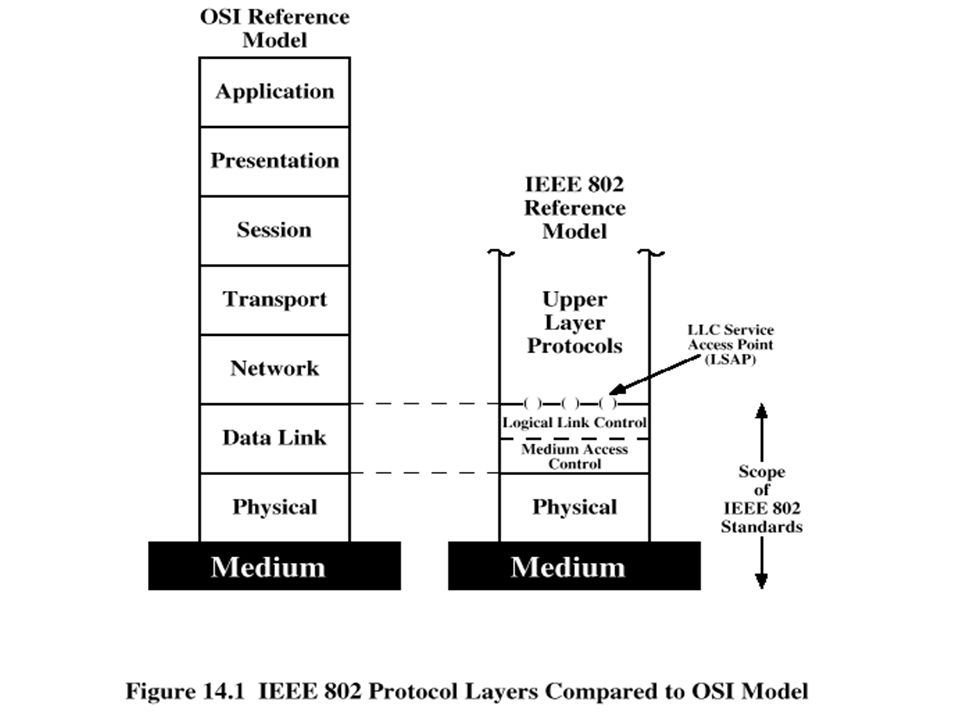
\includegraphics[scale=0.5]{images/802_protocol_layers.jpg}}
\caption{}
\end{figure}

\pagebreak

\subsubsection{IEEE 802.11}
En orden de adaptar Ethernet a redes inalámbricas la IEEE decidió comenzar con el proyecto 802.11. Similarmente como se hizo en 802.3 pero para redes inalámbricas de área local (WLAN), 802.11 determina las especificaciones referentes a la capa física y lógica del modelo OSI para redes wireless. Esto incluye normas y alternativas acerca del rango de frecuencias, velocidad de transmisión, alcance, ancho de banda, y modulación a operar. Estas fueron derivándose con el tiempo de las enmiendas 802.11x, tales como el primero 802.11a, y posteriores 802.11b, 802.11g, 802.11n, y otras mas recientemente incorporadas como 802.11ac y 802.11w.

\begin{figure}[H]
\centerline{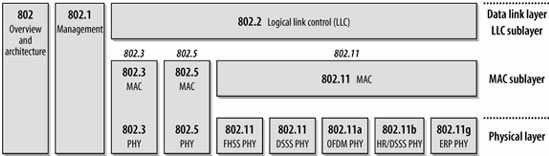
\includegraphics[scale=0.75]{images/802_network_family.jpg}}
\caption{Distribución de estándares 802}
\end{figure}

La necesidad que derivo en la aparición de un nuevo sub árbol del 802 dedicado a redes wireless, fue debido a que lo propuesto en 802.3 no satisfacía ciertas problemáticas que presentan los medios inalámbricos. Para empezar 802.3, si bien es asociado a Ethernet, es mas específicamente un estándar sobre CSMA/CD (Carrier Sense Multiple Access network with Collision Detection). Este esta orientado a detectar posibles colisiones que sucedan al haber dos o mas dispositivos transmitiendo en el mismo canal. No obstante en el caso de wireless el canal no necesariamente permite que todos los nodos involucrados en el puedan escuchar todo lo transferido, esto se a debe a ciertos factores, como que las conexiones son half-duplex. Otro factor es la distancia, si bien 802.11 define un rango de distancia necesario entre dos nodos que pretendan establecer una comunicación, podría ocurrir el problema del nodo oculto, en el cual dos nodos intentan comunicarse con un tercer nodo que puede escuchar a ambos, pero ninguno de los dos primeros puede escuchar al otro.

\begin{figure}[H]
\centerline{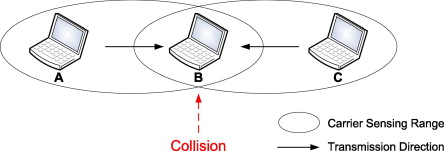
\includegraphics[scale=1.2]{images/hidden_node_problem.jpg}}
\caption{Problema del Nodo Oculto}
\end{figure}

Para mitigar este tipo de problemas es que 802.11 especifica el uso de CSMA/CA (Carrier-sense multiple access with collision avoidance) con RTS/CTS. De esta forma el dispositivo que intente transferir tras esperar a que el medio este en estado idle, y esperar un tiempo predefinido, transmitirá un mensaje de Request to Sent (RTS), y esperada a que el dispositivo al cual se le quiera transmitir conteste con un mensaje de Clear to Sent (CTS), si es que esta listo para recibir, o RxBUSY si es que no lo esta. En este último caso el dispositivo esperara un tiempo pertinente para luego volver a enviar un nuevo RTS, en el otro caso el dispositivo que envió el correspondiente RTS podrá empezar a transmitir, para luego ser informado por medio de un mensaje acknowledge (ACK) por parte del destino si el frame llego correctamente, caso contrario el frame se considera como perdido, lo cual desencadena nuevamente el mismo proceso en orden de reenviar dicho frame, esta perdida podría también ser informada explícitamente por medio de un NACK. Para cada red el uso de RTS/CTS es opcional, pero debido a que en la practica resulta mucho mas eficiente a la hora de eludir colisiones, suele ser el método mas generalizado. 

\begin{figure}[H]
\centerline{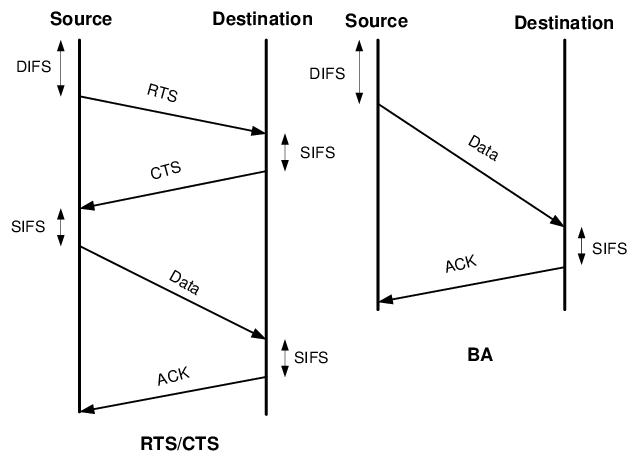
\includegraphics[scale=0.5]{images/BA_and_RTSCTS_methods_handshake.jpg}}
\caption{Esquema de envio de datos de 802.11}
\end{figure}

En orden de entender este intercambio como una operación atómica, es necesario entender la noción de \textit{coordination functions}, y \textit{carrier-sensing functions}. Las \textit{coordination functions} son mecanismos que dictaminan cuanto debe esperarse en cada situación para poder enviar un paquete a la red. Típicamente este mecanismo es especificado por la \textit{distributed coordination function (DCF)}, pero también existen otras alternativas menos difundidas como la \textit{point coordination function (PCF)} que trabaja sobre DCF. DCF es quien provee el mecanismo CSMA/CA, generalmente junto con RTS/CTS, de manera que a la hora de intentar acceder al medio primero espera un breve intervalo de tiempo llamado \textit{interframe space}, si durante ese tiempo el medio estuvo en estado \textit{idle}, se esperada un intervalo extra de tiempo llamado \textit{contention window} o \textit{backoff window}, este intervalo es dado por la elección aleatoria de cierto \textit{slot} de tiempo entre un rango de \textit{slots} generado por el algoritmo de \textit{exponential backoff} (que indica un rango de \textit{slots} entre  $0$ y $2^{c} - 1$, donde $c$ es la cantidad de colisiones/perdidas de paquetes), en caso contrario, en el que el medio este ocupado, volverá a realizar dichas esperas. El \textit{interframe space} se determina de acuerdo al tipo de paquete a enviar, y estará ligado a la prioridad de los mismos. Por ejemplo, los paquetes de control tales como los RTS, CTS y acknowledges, tendrá que esperar un intervalo \textit{SIFS} (short interframe space), mientras que para iniciar una nueva ráfaga de fragmentos se tendrá que esperar un intervalo de \textit{DIFS} (DCF interframe space). A su vez para que las \textit{coordination functions} sepan si el canal está ocupado o no, es que son necesarias las \textit{carrier-sensing functions}. Existen dos tipos de ellas, en primer lugar están las \textit{physical carrier-sensing functions} que identifican al medio ocupado en base a la detección a nivel físico del uso del canal, en segundo lugar y debido a obstáculos ya mencionados como el \textit{hidden node} y las limitaciones de las conexiones \textit{half duplex}, es que entran en juego las \textit{virtual carrier-sensing functions}. Estas últimas identifican al canal como ocupado en base los \textit{Network Allocation Vector} (NAV) recibidos. El NAV es un valor continuamente actualizado en los nodos de la red que registra por cuanto se quiere reservar el canal para poder enviar el próximo frame, este incluye los tiempos asociados al intercambio de mensajes de control necesarios para el envío de dicho frame. Para esto el \textit{header} de los paquetes 802.11 provee un campo de \textit{duración/ID} en donde suele almacenarse dicho valor, aunque suele compartir el espacio para otros significados, como el que le dan ciertos paquetes de gestión tales como los paquetes de \textit{beacon}. Los paquetes 802.11 a su permiten una longitud variable del \textit{payload}, permitiendo fragmentar los paquetes de las capas superiores en fragmentos arbitrariamente largos (dentro de ciertos rangos permitidos), de manera que el envío de un \textit{frame} puede significar el envío de una ráfaga de fragmentos que comparten el mismo número de secuencia de frame, pero distinto número de fragmentación, el cual permite al receptor ensamblar los fragmentos en orden, y tratarlo atómicamente como un frame. Esta técnica de fragmentación suele ser muy útil para mejorar el \textit{throughput} en medios de mucho ruido, ya que la pérdida de un fragmento a causa de este no significaría la perdida de todo el paquete, haciendo necesario reenviar solo el fragmento perdido. El inconveniente de la fragmentación es la enorme cantidad de \textit{overhead} de datos de control generados, incluyendo los encabezados que viajan en cada fragmento, por lo que en ambientes con una medida de ruido aceptable es recomendable utilizar otras técnicas como la agregación, por la cual se empaquetan en un solo frame más extenso con una cabecera común, a varios \textit{payloads} separados por una cabecera mínima.


\begin{figure}[H]
\centerline{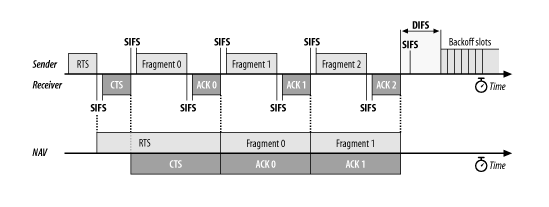
\includegraphics[scale=0.8]{images/80211_fragmentation_burst.png}}
\caption{Fragmentacion}
\end{figure}

Los paquetes 802.11 se dividen esencialmente en tres segmentos, una primera sección de encabezado llamada \textit{MAC Header}, una sección de \textit{payload} llamada \textit{Frame Body}, y una última sección llamada \textit{Frame Check Sequence}. La sección de \textit{MAC Header} a su vez está compuesta por 7 campos, el\textit{Frame Control}, que contiene información básica de control, el \textit{Duration/ID} que ya hemos comentado, luego le siguen 4 campos de dirección, y uno de control llamado \textit{Sequence Control}, que como su nombre sugiere, almacena el número de fragmento y numero de secuencia (que identifica al frame fragmentado). Los campos de dirección varían su uso y significado dependiendo del tipo de paquete, un típico paquete de datos usara el primer campo para la dirección MAC de la estación receptora, el segundo para la dirección MAC transmisora, la tercera para la MAC de destino, y la cuarta para la MAC de origen, no obstante, un paquete de control como los CTS solo harán uso del primer campo para la dirección del receptor, que es el único uso común de este campo para todos los paquetes. La dirección receptora y transmisora podrían diferir de la de origen y destino respectivamente, puesto que las primeras refieren a las direcciones del nodo actual que está propagando el paquete hacia el próximo salto, mientras que la dirección de origen refiere a la MAC del dispositivo que originalmente genero el paquete, y la de origen a la MAC del destinatario del mismo. 

Examinando como mayor detalle, el campo de \textit{Frame Control} se divide a su vez en 11 campos, el campo \textit{Protocol} indica la versión de 802.11 usada para ese frame, hoy en día se sigue usando una única versión, por lo que este permanece en $00$. El campo de tipo y de subtipo (\textit{Type} y \textit{Subtype}) indican el tipo de paquetes que representa el frame, 802.11 se maneja con 3 tipos básico de frames, los de datos, los de gestión, y los de control, de este último tipo ya hemos visto ejemplos (RTS, CTS y Acknowledge). Mas específicamente el campo \textit{Type} indica a cuál de estas tres categorías corresponde el paquete, y el campo \textit{Subtype} cuál de los posibles paquetes de esa categoría se corresponde, por ejemplo, los RTS tiene al valor $1011$ como subtipo. los campos \textit{to DS} y\textit{from DS} indican si el frame está dirigido al \textit{distribution system} (DS) o no, por ejemplo, en modo infraestructura los paquetes dirigidos a los dispositivos que no funcionen como \textit{bridge} serán enviados con el\textit{to DS} igual a $0$ y el \textit{from DS} igual $1$. El campo \textit{More fragments} indica si el frame fue fragmentado y se esperan más fragmentos a ser recibidos. El campo \textit{Retry} indica si el frame está siendo retransmitido (por ejemplo, porque no recibió el ACK del original u otro anterior). Las estaciones conectadas a la red pueden informar al \textit{access point} que podrán en modo de bajo consumo, para esto utilizan el campo \textit{Power Management}, en este modo el \textit{access point} retendrá en un \textit{buffer} algunos paquetes enviados para la estación en cuestión, y luego le informara a la estación mediante el campo \textit{More Data} que tiene en su \textit{buffer} al menos un paquete para él. Este último también es usado por el \textit{access point} para indicar que más frames de tipo \textit{multicast/broadcast} serán enviados. Con la incorporación de la rutina de encriptación WEP, se reservó el campo \textit{Protected Frame} para indicar que el frame estaba protegido, aunque hoy en día solo con el uso de WEP no debería considerase así, esto lo discutiremos más adelante en la sección de WEP. Por último, en el \textit{header} nos encontramos con el campo \textit{Order} o "strict ordering delivery" que indica que obligatoriamente el frame debe ser procesado en el orden en el que se transmitió.

A continuación del \textit{MAC header} se encuentra \textit{Frame Body}, este es el contenido del paquete propiamente dicho, en el caso de los frame de datos este contiene los datos a ser enviados y recibidos por la capa superior en la estación receptora, en el caso de los frames de control y gestión, este contiene otros campos propios del tipo de paquete asociado al indicado en el campo \textit{Type} y \textit{Subtype}. Por último, el \textit {Frame Check Sequence} es un valor generado a partir de realizar un chequeo de redundancia llamado\textit{cyclic redundancy check} (CRC) sobre los campos del \textit{MAC header} y \textit{Frame Body}, con el la estación receptora podrá comprobar con cierta probabilidad si el paquete no sufrió algún daño durante la transmisión al correr el mismo procedimiento sobre dichos campos.


\begin{figure}[H]
\centerline{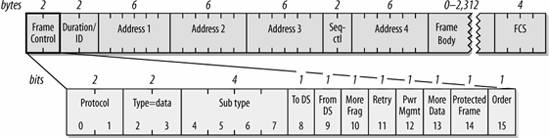
\includegraphics[scale=0.8]{images/8011_format_frame.png}}
\caption{Formato de frame 802.11}
\end{figure}

Por último, explicaremos algunos tipos de paquetes de gestión que juegan un rol importante a la hora de acceder a una red \textit{WiFi}. Para estos se lleva a cabo un procedimiento que consta de dos partes, autenticación, y asociación. Los \textit{access point} a no ser que estén configurados para lo contrario, suelen propagar sobre su rango de cobertura cada cierto intervalo de tiempo, un tipo de paquetes llamados \textit{beacon} que contiene información básica de las características configuradas de para esa red, tales como su SSID, su propósito principal es anunciar la existencia de la red a los posibles dispositivos que estén escuchando el medio en busca de algún \textit{access point} al cual conectarse. Tras recibir este tipo de paquetes, las estaciones que buscan acceso enviaran un mensaje de \textit{Probe Request} a cada \textit{access point}, que contiene el correspondiente SSID, y los tipos \textit{rates} soportados. Si el \textit{access point} considera en base a esta información que la estación es compatible, responde con un mensaje de tipo \textit{Request Response}, que contiene los datos del \textit{beacon} asociado. Una vez recibidos estos paquetes, la estación receptora elegirá alguno de los \textit{access point} que respondieron, en base a algún criterio (ya sea por mejor señal, o algún criterio pre-configurado), y comenzara el proceso de autenticación por medio de un paquete de tipo \textit{Authentication} que entre otros datos especifica el tipo de algoritmo de autenticación a usar por medio del campo \textit{Authentication Algorithm Number}. 

802.11 de por sí solo ofrece dos algoritmos de autenticación, \textit{Open System Authentication} y \textit{Shared Key Authentication}, al que les corresponden el número $0$ y $1$ respectivamente. En el caso de \textit{Open System Authentication}, debido a que no se realiza ningún chequeo de identidad el sistema está abierto a todo aquello que quiera acceder, simplemente tras recibir el paquete de tipo \textit{Authentication} el \textit{access point} responderá con otro paquete del mismo tipo, en el cual incluirá en un campo de \textit{Status Code} el resultado del intento de autenticación. En contraste a este, \textit{Shared Key Authentication} fue diseñado para ser usado con el \textit{Wired Equivalency Privacy} (WEP), y así otorgar acceso solo a aquellos usuarios que conozcan una única clave compartida entre todos ellos y el \textit{access point}. Para ello al igual que antes envía un paquete de tipo \textit{Authentication} al \textit{access point}, pero en este caso en vez de autenticarlo sin ningún chequeo, envía un \textit{challenge}, más precisamente un texto de 128 bytes generado aleatoriamente usando el \textit{WEP keystream generator}. La idea detrás de esto es que el cliente reenvíe este texto, pero cifrándolo con la clave compartida, de este modo el \textit{access point} al conocer la misma clave podrá realizar el mismo procedimiento y comprobar si la respuesta corresponde al texto cifrado con esa misma clave, si es así, esto significaría que el cliente conoce esa clave secreta, por ende, se le otorga el acceso.

En caso de que el proceso de autenticación haya sido satisfactorio, pasa a realizar una segunda etapa, la de asociación, que consiste en asociar al cliente con algún \textit{access point} en particular, si previamente a esta etapa no se concretó la autenticación se le enviada al cliente un paquete de tipo \textit{Deauthentication}, de modo que este tendrá que comenzar nuevamente el proceso de autenticación. Para esta etapa solo es necesario un intercambio de paquetes de tipo \textit{Association Request} y \textit{Association Respond}, por el cual se le asigna al cliente un \textit{association ID}.

\begin{figure}[H]
\centerline{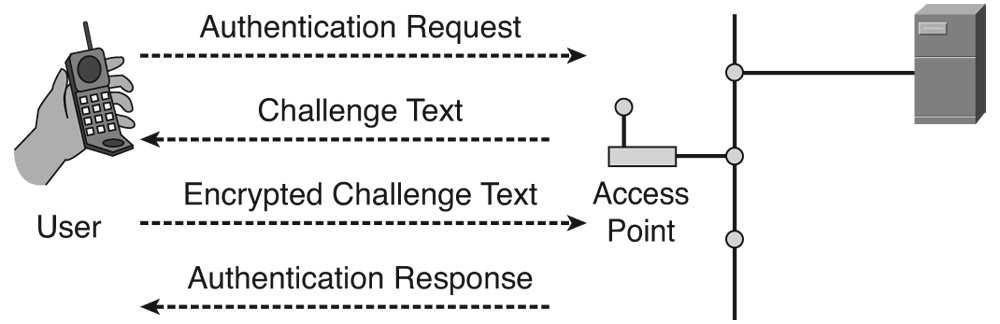
\includegraphics[scale=0.4]{images/80211_shared_key_authentication.jpg}}
\caption{Autenticación 802.11 por medio de \textit{Shared Key Autentication}}
\end{figure}

Debido a las debilidades del mecanismo ofrecido mediante el \textit{Shared Key Authentication} que se explicaran posteriormente, y a la falta de restricción de usuarios del \textit{Open System Authentication}, fue necesario mediante la incorporación de nuevos sistemas \textit{ad-hoc} de autenticación. Para lo cual se emplea de manera difundida los protocolos WPA y WPA2 especificados en 802.11i. A su vez estos protocolos utilizar un versátil protocolo de autenticación llamado EAP, mediante su encapsulamiento dentro paquetes EAPoL. 

\subsubsection{Extensible Authentication Protocol over LAN (EAPoL)}

En orden de conseguir un mecanismo de autenticación estándar se diseñó el protocolo de \textit{Extensible Authentication Protocol} (EAP). Debido a que este protocolo fue diseñado inicialmente para funcionar sobre el protocolo \textit{Point-to-Point Protocol} (PPP), fue necesario realizar ciertos agregados para poder adaptarlo a redes LAN. Para esto se diseñó el protocolo \textit{Extensible Authentication Protocol over LAN} (EAPoL), básicamente este concibe un encapsulamiento a los paquetes EAP, de manera que para los procesos de autenticación en redes 802.11 los paquetes EAP son almacenados en el campo de \textit{payload} de paquetes EAPoL, y estos a su vez viajan encapsulados en el \textit{payload} de los paquetes 802.11.


%\begin{figure}[H]
%\centerline{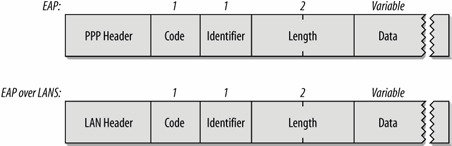
\includegraphics[scale=0.8]{images/EAPoL_format.jpg}}
%\caption{}
%\end{figure}

Examinando más en detalle los paquetes de EAP, se evidencia el motivo de la necesidad de EAPoL, para empezar estos no tienen un encabezado MAC, debido a que fue diseñado para una red punto a punto (de solo dos nodos) no fue necesario el uso de direcciones fuente ni origen, por lo que para subsanar este problema los paquetes de EAPoL comienzan con este encabezado faltante. Concretamente los paquetes EAP están compuestos por 4 campos, el campo \textit{Code} específica a qué tipo de paquete EAP corresponde, lo cual es necesario para interpretar el ultimo campo de datos \textit{Data}, en el intercambio de estos paquetes este código indica si se trata de un \textit{Request}, o un \textit{Response}. Además de esto se incluye un campo de identificación \textit{Identifier}, que relaciona mediante un numero un paquete de \textit{Request} con su respectivo paquete de \textit{Response}, y un campo de longitud, que determina el tamaño del campo de datos. Mientras que los paquetes EAPoL además del encabezado ya mencionado, están compuesto por otros 6 campos, el de \textit{Ethernet Type} contiene el código asignado a este tipo de paquetes (el 88-8e), el campo \textit{Version} que indica la versión del protocolo a la que pertenece el paquete, al igual que los paquetes 802.11 este posee \textit{Frame Check Sequence} al que se le da el mismo uso. Para poder transportar los paquetes EAP también posee un campo de \textit{payload} llamado \textit{Packet Body}, al que también se le asocia una longitud especificada en el campo \textit{Lenght}. Existen varios tipos de paquetes EAPoL con distintos propósitos, para identificar cada uno se utiliza un campo de \textit{Packet Type} que almacena el código asociado al tipo de paquete correspondiente.

\begin{figure}[H]
%\centerline{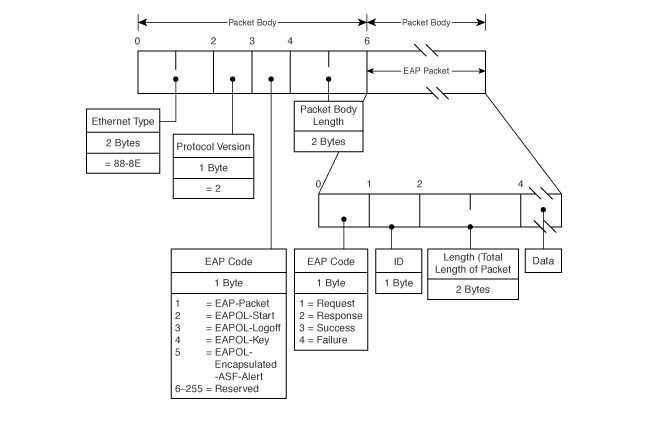
\includegraphics[scale=0.8]{images/EAPoL_and_EAP_packets.jpg}}
\centerline{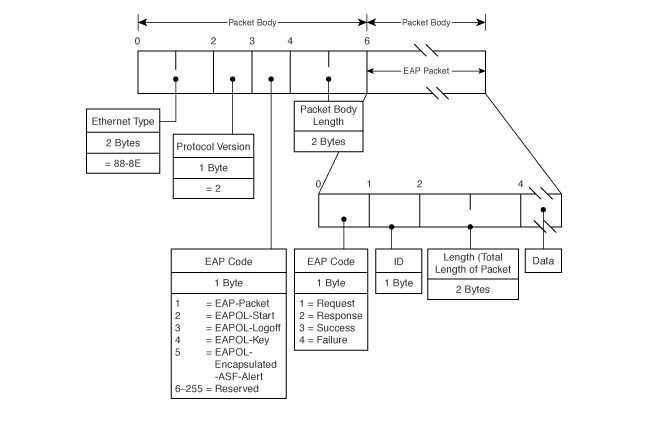
\includegraphics[width=20cm,height=10cm]{images/EAPoL_and_EAP_packets.jpg}}
\caption{Formato de frame EAPoL y EAP contenido}
\end{figure}

La incorporación de estos paquetes a las redes LAN fue presentada mediante 802.1x quien ofrece un nuevo mecanismo de autenticación para estas redes, que se emplea después de la etapa de autenticación y asociación clásica de 802.11. 802.1x introduce tres componentes que juegan distintos roles a la hora de autenticarse, en primer lugar se tiene al \textit{Supplicant} que refiere a quien quiere autenticarse, en segundo lugar se tiene a la entidad encargada de orquestar el proceso de autenticación, el \textit{Authenticator}, y por último se tiene a un \textit{Authentication Server} quien es el encargado de efectivamente en base a las credenciales enviadas por el \textit{Supplicant} decidir si se le otorga el acceso y bajo qué condiciones. Tanto el \textit{Supplicant} como el \textit{Authenticator} son referidos como \textit{Port Authentication Entities} (PAEs), los cuales son puertos lógicos que desempeñan dichos roles, y varían su comportamiento de acuerdo al estado en que se encuentren. Los PAEs pueden encontrarse en dos estados, \textit{uncontrolled} y \textit{controlled}. Para las estaciones que no hayan finalizado la autenticación, el puerto del \textit{Authenticator} permanecerá en estado \textit{uncontrolled}, con lo cual solo aceptará cierto tipo de paquetes como los EAPoL, y descartada muchos otros como los típicos paquetes de datos, mientras que para los dispositivos ya autenticados el puerto permanecerá en estado \textit{controlled}, pudiendo usar la red normalmente sin dicha restricción. Si bien este es el modelo clásico existen \textit{access points} que pueden desempeñar tanto el rol de \textit{Authenticator} como el rol de \textit{Authentication Server}.

El proceso de autenticación es similar a la autenticación de EAP, pero no idéntico, para empezar 802.1x permite que el \textit{Supplicant} dispare el proceso de autenticación mediante un paquete de tipo \textit{EAPoL-Start}, mientras que en EAP el inicio del proceso es disparado por el \textit{Authenticator}, no obstante, una vez enviado el \textit{EAPoL-Start} el proceso continúa como una autenticación estilo \textit{EAP}. El \textit{Authenticator} le responde al \textit{Supplicant} con un paquete de \textit{Request} de tipo \textit{EAP-Identity}, solicitando información de identificación, el \textit{Supplicant} responde por medio de un paquete de \textit{Response} de tipo \textit{EAP-Identity}. 


Luego el \textit{Authenticator} debe comunicarse con el \textit{Authentication Server}, para lo que emplean un protocolo llamado RADIUS. El proceso continúa con un mensaje RADIUS de tipo \textit{Access Request} de parte del \textit{Authenticator} hacia el \textit{Authentication Server} en el que envía los datos identificatorios del \textit{Supplicant}, para luego responder con un paquete de tipo \textit{Request Challenge}. Dependiendo del método de autenticación, se enviará un mensaje al \textit{Supplicant} un mensaje de \textit{Request} con el código asociado a él, por ejemplo, MD5, TLS, u OTP. Luego se procederá con otro intercambio similar entre el \textit{Supplicant}, el \textit{Authenticator}, y el \textit{Authentication Server}, para validar la respuesta del \textit{challenge}, solo que en esta vez la respuesta del servidor será un paquete de tipo \textit{Access Acepted} o \textit{Access Rejected}, según se le haya permitido o no el acceso. Finalmente, el \textit{Authenticator} informada la decisión al \textit{Supplicant} por medio de un paquete EAP de tipo \textit{Success} o \textit{Failure} según corresponda.

EAPoL también ofrece otros tipos de paquetes como el \textit{EAPoL-LogOff} que permiten des autenticarse de la red, y los \textit{EAPoL-Key} para intercambiar información de claves criptográficas, como sucede por ejemplo en el WPA \textit{4-way-handshake}.

\begin{figure}[H]
\centerline{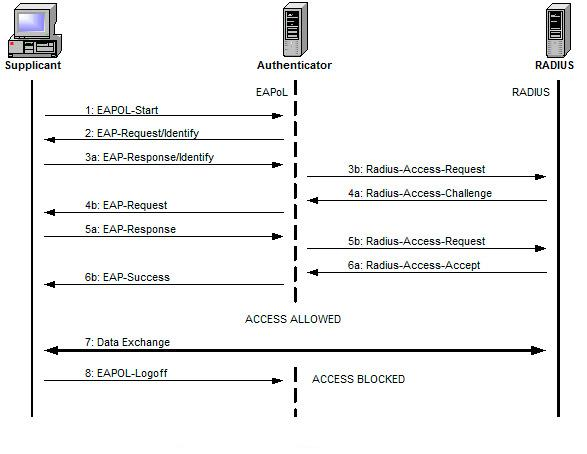
\includegraphics[scale=0.7]{images/8021x_handshake.jpg}}
\caption{handshake 802.1x}
\end{figure}

\pagebreak

\subsubsection{Wired Equivalent Privacy (WEP)}

Este el mecanismo inicial que ofreció 802.11 con el objetivo de garantizar confidencialidad a redes de área local.
A diferencia de sus sucesores WEP nunca negocia una clave de encriptación al momento de acceder a la red, ni tampoco tras cierto periodo de tiempo, simplemente se basa en el uso de una clave común llamada \textit{WEP-Key} prestablecida en todos aquellos que pretendan interconectarse a la red protegida por medio de WEP. Tras la autenticación WEP por medio de un \textit{challenge}, las comunicaciones bajo este protocolo son encriptadas por medio de una clave que resulta de un \textit{Initial Vector} (IV) y la \textit{WEP-Key} que se concatenan y sirven de entrada a un módulo de RC4 que genera una \textit{Key stream} la cual es aplicada a una función de XOR junto con el resultado de concatenar el texto en claro a un valor de integridad \textit{Integrity Check Value} (ICV), que fue generado previamente en base al texto en claro.

\begin{figure}[H]
\centerline{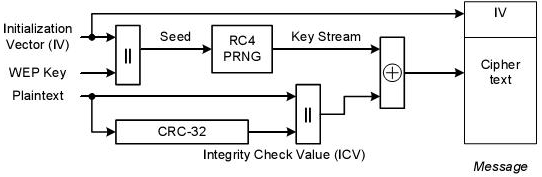
\includegraphics[scale=0.7]{images/wep_mechanism.png}}
\caption{Mecanismo de encriptación de WEP}
\end{figure}

Nótese que durante este proceso a diferencia de otros mecanismos no se realiza ningún método particular de autenticación. Otro punto crucial es que la \textit{WEP-Key} al no ser actualizada a otro valor durante la transmisión compromete la seguridad basada en RC4, debido a que aún con el vector inicial mutando en el tiempo, la posición y tamaño de ambos parámetros no varía, y en consecuencia debido a la poca longitud de la clave, no es difícil en base a suficientes paquetes recolectados deducir la \textit{WEP-Key}. En consecuencia, cualquier red con este tipo de mecanismos de seguridad es plenamente vulnerable, por lo que hoy en día este protocolo se considera deprecado.


\subsubsection{WIFI Protected Access (WPA)}
Debido a los problemas de seguridad que el ya establecido WEP acarreaba, se decidió desarrolla 802.11i, el cual aporta a 802.11 sistemas más robustos de seguridad. Si bien la idea original fue desarrollar un nuevo y único protocolo de encriptación, debido a la urgencia transmitida por la industria que clamaba por una nueva alternativa al vulnerable WEP, se desarrolló una versión superadora de éste como solución a corto plazo llamado WPA y tras este, tiempo después vendría la solución a largo plazo que se esperaba dar desde un principio, al que se le llamo WPA2. La diferencia entre ambos radica en el protocolo de integridad y confidencialidad utilizado, WPA emplea \textit{Temporal Key Integrity Protocol} (TKIP), mientras que WPA2 utiliza \textit{Counter Mode Cipher Block Chaining Message Authentication Code Protocol} (CCMP), aunque opcionalmente soporta el uso de TKIP. Debido a que TKIP ha presentado varias vulnerabilidades hoy en día se lo considera deprecado, por lo que WPA2 con CCMP suele ser la configuración más difundida.

La encriptación mediante de TKIP se basa en el mecanismo utilizado en WEP el cual hace uso del \textit{cipher} RC4, pero en este caso en vez de utilizar 64bits utiliza 128bits. Además, el vector utilizado en RC4 no nace directamente de la concatenación de la \textit{Temporal Key} (TK) junto a un \textit{Initail Value} (IV) como sucedía antes, sino que se genera mediante una función de \textit{hashing} que toma como entrada a la TK junto a un número de secuencia \textit{TKIP sequence} (TSC) que inicia en cero y luego es incrementado con cada \textit{frame} enviado. Por otro lado, al bloque formado por las direcciones de origen y destino, el campo de prioridad, y el \textit{payload} que representan al \textit{frame} en sí, le es concatenado el MIC al ser procesado junto a una clave dedicada de MIC derivada de la PMK. El resultado de esto es tratado como el texto en claro a ser procesado por el mecanismo de WEP, junto al IV generado en el primer procedimiento.

La encriptación mediante CCMP a diferencia de TKIP y WEP ya no hace uso de RC4, sino que utiliza AES de manera anidada, al cual se lo considera un \textit{cipher} más seguro. Este mecanismo constituye una primera etapa de cálculo de MIC, y una segunda etapa de encriptación del \textit{payload} y el MIC previamente calculado. Para calcular el MIC se introduce a un primer bloque inicial que se deriva de ciertos campos del \textit{frame}, junto a una clave de integridad derivada de la PMK para formar un bloque de 128bits que será la entrada del primer módulo de AES. A la salida de este se le aplica una función de XOR junto a los primeros 128bits del \textit{frame}, y al resultado se le vuelve a aplicar un módulo de AES. Este procedimiento continúa a lo largo de todo el \textit{frame} tomando en cada paso a salida del módulo de AES previo y los próximos 128bits del \textit{frame}, para lo que previamente se le adjunto alrededor del campo de datos ciertos segmentos de \textit{padding} para garantizar que el \textit{frame} tenga una longitud múltiplo de 128bits. Al terminar con los últimos 128bits del \textit{frame}, la salida del módulo AES correspondiente devolverá un nuevo segmento de 128bits de los cuales se utilizará los primeros 64 como valor del MIC. En una segunda etapa el \textit{payload} del \textit{frame} es efectivamente encriptado, para lo cual similarmente a lo hecho en la primera etapa se vuelve a construir un nuevo vector inicial de 128bits por medio de la concatenación de la TK a la cola de un bloque inicial derivado de la dirección de origen, el campo de prioridad, un \textit{nonce} también conocido como \textit{Packet Number} (PN), y otros campos de control del \textit{frame}. Este vector inicial se utiliza en las entradas de los módulos AES para luego aplicarle a la salida del mismo una función de XOR a los 128bits del segmento correspondiente del \textit{payload} del \textit{frame}. En orden de no utilizar el mismo vector inicial para cada módulo, a dicho vector se lo incrementa en 1 por cada segmento de 128bits recorrido hasta ese momento (incluyendo el actual). Durante este procedimiento además se encripta el campo de MIC anexado en la etapa anterior a la cola del \textit{frame}.

\begin{figure}[ht]       
    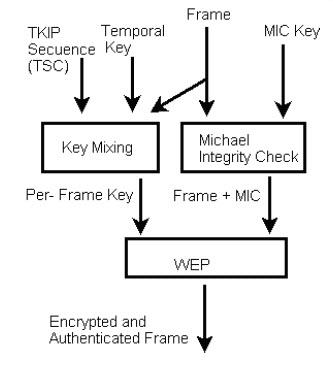
\includegraphics[scale=0.6]{images/tkip_encription.jpg}   
    \hspace{10px}
    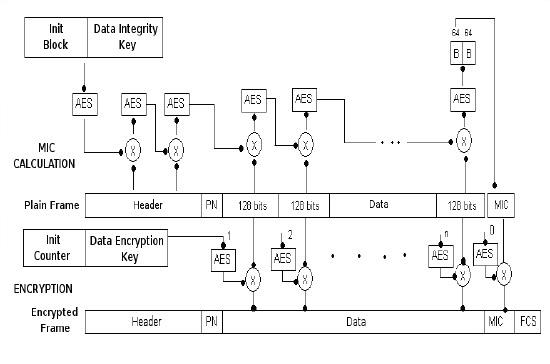
\includegraphics[scale=0.8]{images/ccmp_encription.jpg}
    \caption{Encriptación por medio de TKIP (izquierda) y por medio de CCMP (derecha)}
\end{figure}

El proceso de autenticación a una red con seguridad WPA/WPA2 comienza esencialmente por cuestión de compatibilidad de la misma manera que ocurría en el clásico 802.11, mediante una primera etapa de autenticación y una segunda etapa de asociación. La etapa de autenticación se realiza mediante \textit{Open System Authentication}, que funciona más como una formalidad o método para intercambiar información pública (como las direcciones MAC), ya que la autenticación real de WPA/WPA2 sucede a continuación de estas dos etapas. Para la siguiente etapa 802.11i ofrece dos modos de autenticación, \textit{Pre-Shared Key} y \textit{Enterprise}. La principal diferencia entre ambos es como se deriva la \textit{Pairwise Master Key} (PMK); en \textit{Pre-Shared Key} esta deriva de un secreto compartido, relacionado con lo que conocemos cotidianamente como \textit{password} de la red. Mientras que en el modo \textit{Enterprise}, esta se negocia dinámicamente de acuerdo a las credenciales entregadas al \textit{Authentication Server} por medio de un proceso de autenticación 802.1x. Este último modo se considera más seguro, debido a que, en caso de algún acceso ilícito a ciertas credenciales individuales, solo será comprometido el tráfico de ese usuario en particular. En ambos modos de operación tras el proceso de autenticación, ya sea solo por medio de \textit{Open System Authentication} en modo \textit{Pre-Shared Key}, o además de este por autenticación 802.1x, se realiza propiamente los procesos de generación de claves, estos son el \textit{4-way handshake} y \textit{group key handshake}, ambos por medio de intercambios de paquetes \textit{EAPoL-Key}.

El \textit{4-way handshake} es el intercambio de mensajes por el cual el \textit{Supplicant} se autentica por medio del uso de un secreto compartido con el \textit{Athenticator}, la PMK. Durante este proceso además se negocia una nueva \textit{Pairwise Transient Key} (PTK), la cual nace en base a 5 valores, la PMK, la MAC de \textit{Supplicant}, la MAC del \textit{Authenticator}, y otros dos valores que se generan aleatoriamente a la hora de realizar el \textit{4-way handshake} llamados \textit{nonce}. Además, durante este proceso el \textit{Athenticator} le transmite la \textit{Group Transient Key} (GTK), con la cual se encriptan los datos de los paquetes \textit{broadcast}, y debido a esto todos los nodos autorizados de la red deben conocerla. A la hora de iniciar el \textit{4-way handshake} la PMK, y las direcciones MAC del \textit{Suplicant} y \textit{Authenticator} ya son conocidas, por lo que solo es necesario intercambiar los \textit{nonce}. El primer paso del \textit{4-way handshake} consiste en el envío por parte del \textit{Authenticator} de un paquete \textit{EAPoL-key}, el cual contiene en el campo \textit{nonce} el primer \textit{nonce} referido comúnmente como \textit{Anonce}. Con este valor el \textit{Supplicant} genera el segundo \textit{nonce} referido como \textit{Snonce}, con lo cual ya posee los 5 valores necesarios para generar la PTK.
Una vez generada la PTK, esta se divide en otras 3 claves con propósitos específicos, la \textit{Key Confirmation Key} (KCK), la \textit{Key Encription Key} (KEK), y la \textit{Temporal Key} (TK). La TK es la clave con la cual efectivamente se encripta los datos enviados por las capas superiores, la KEK es la clave con la cual se encripta cualquier otra clave enviada, que viajan en el campo de datos de los paquetes \textit{EAPoL-Key}, por último la KCK se utiliza junto a una función de HMAC para generar un \textit{hash} llamado \textit{Message Integrity Control} (MIC), el cual es almacenado en el campo de \textit{MIC} de los paquetes \textit{EAPoL-Key}. Estos MIC se utilizan para confirmar la autenticidad del paquete enviado, por lo que se usa en todos los paquetes enviados durante el \textit{4-way handshake} y el \textit{group handshake}, con la excepción del primer envío ya explicado (debido a que en ese momento aún no se puede derivar la KCK).

\begin{figure}[H]
\centerline{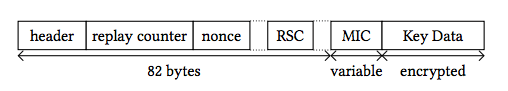
\includegraphics[scale=0.7]{images/EAPoL_key_format.png}}
\caption{Formato del frame EAPoL-Key}
\end{figure}

Continuando con el \textit{4-way handshake}, el \textit{Supplicant} envía el \textit{Snonce} al \textit{Authenticator} para que este también pueda derivar la PTK. Si el resultado de realizar el HMAC sobre el \textit{Snonce} recibido usando la KCK que resulta de la PTK derivada para ese mismo \textit{Snonce}, concuerda con el MIC del paquete en el que viajo el \textit{Snonce}, el \textit{Authenticator} supone que efectivamente el \textit{Snonce} vino de una estación que conoce la PMK, puesto que sino no podría haber derivado correctamente la KCK. Posteriormente el \textit{Authenticator} envía un paquete \textit{EAPoL-Key} conteniendo en el campo de datos a la GTK encriptada con la KEK, y en el campo de MIC el resultado del HMAC del paquete utilizando además la KCK. Del lado del \textit{Supplicant} se comprueba la autenticidad del paquete, por medio de la KCK, y se descifra la GTK utilizando la KEK. Por último, el \textit{Supplicant} envía un mensaje de confirmación junto su MIC asociado, e instala la PTK. La misma instalación ocurre del lado del \textit{Authenticator} al llegar ese último mensaje. Nótese que la derivación de la nueva PTK no es lo mismo que su instalación, cada cierto tiempo el \textit{4-way handshake} vuelve a realizarse de la misma forma, utilizando la TK, KEK y KCK, hasta ese momento conocidas, y se actualizarán recién al instalar la nueva PTK (y no solo al derivarla). A su vez es posible actualizar la GTK sin actualizar aun la PSK, por medio de un \textit{handshake} dedicado llamado \textit{group key handshake}, el cual constituye esencialmente los últimos dos intercambios del \textit{4-way handshake}.

\begin{figure}[H]
\centerline{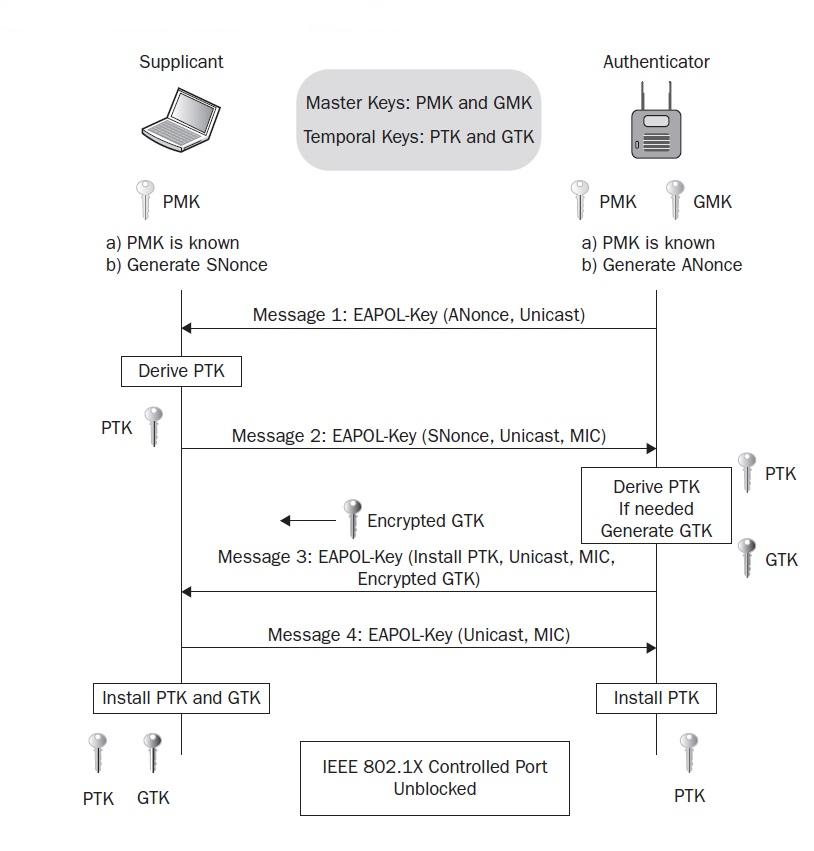
\includegraphics[scale=0.5]{images/4Way-Handshake.jpg}}
\caption{802.11i 4Way-Handshake}
\end{figure}

\subsection{Ataques}

\subsubsection{Key Reinstallation Attacks (KRACK)}

KRACK refiere es una familia de ataques que fueron publicados por Mathy Vanhoef en el paper \textit{Key Reinstallation Attacks: Forcing Nonce Reuse in WPA2} el 11 de noviembre del 2017. Como su nombre sugiere este tipo de ataques consisten en forzar la reinstalación en la estación objetivo de la PTK o de la GTK según se trate. Para esto los ataques de KRACK requieren como precondición no solo que estemos en una posición de MiTM, con respecto a la estación y \textit{access point} objetivos, sino que para además esto le sea completamente transparente a ambos. Por esta razón no cualquier técnica de MiTM es aplicable, en particular para la presentación de estos ataques se propuso usar \textit{based-channel MiTM}.

Debido a la potencial amenaza de métodos de deducción de claves que rondaban a WEP, 802.11i estableció que cada cierto intervalo de tiempo prudente las estaciones conectadas y el \textit{access point} deberán realizar nuevamente el \textit{4-way handshake} y el \textit{group key handshake} con el motivo de actualizar la PTK, y GTK respectivamente. Si bien esta técnica es conceptualmente favorable, por cuestiones de falta de especificación o detalles de implementación en cada producto, esto derivo en una nueva familia de ataques orientadas a explotar este mecanismo con el fin de persistir claves, o permitir ataques de \textit{replay}. Debido a que no todos estos productos siguen el protocolo al pie de la letra, o simplemente interpretan de distinto modo ciertas cuestiones no especificadas, existen distintas variantes de estos ataques.

Para efectuar los ataques de reinstalación de la PSK el atacante estando ya en posición de MiTM, intercepta y retiene los mensajes entre el \textit{Supplicant} y el \textit{Athenticator} utilizados en el \textit{handshake}. Los primeros 3 mensajes son reenviados de manera transparente, y además una copia del tercero es registrada por el atacante para su posterior uso. A diferencia de estos el cuarto mensaje (enviado por el \textit{Supplicant}) es retenido, de esta manera la recepción e instalación de la PTK y GTK por parte del \textit{Supplicant} no es confirmada por el \textit{Authenticator} mediante la recepción de dicho mensaje. En consecuencia, el \textit{Authenticator} asume que posiblemente el tercer mensaje se haya perdido, por lo que se encarga de retransmitirlo aumentando su contador de \textit{replay}. El \textit{Supplicant} mientras tanto ya habiendo instalado la PSK y la GTK tras la recepción del tercer mensaje, enviará todos los paquetes de datos subsiguientes encriptados con la nueva TK y un \textit{nonce} o secuencia inicial utilizados en los mecanismos de encriptación de los protocolos de confidencialidad de datos (TKIP o CCMP). Oportunamente el atacante reenviará el tercer paquete que fue reenviado por el \textit{Authenticator}, haciendo que el \textit{Supplicant} reinstale la misma PSK y GTK. En consecuencia, a esta reinstalación el \textit{nonce} mencionado anteriormente será inicializado nuevamente a su valor original (siendo este el valor 1), forzando al protocolo de confidencialidad de datos a rehusar el mismo bloque o secuencia inicial del cual se basa el mecanismo de encriptación, que normalmente es incrementado para evitar el reúso de la misma clave.

\begin{figure}[ht]       
    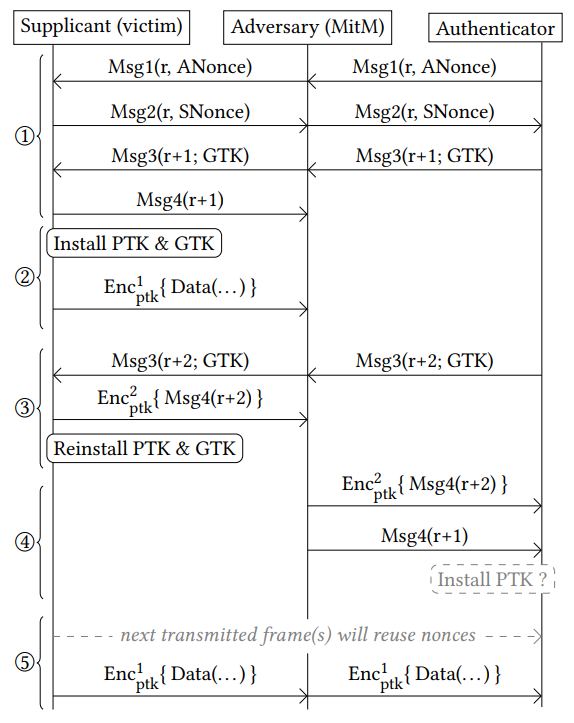
\includegraphics[scale=0.4]{images/krack_supplicant_still_accept_plaintext.png}
    \hspace{10px}
    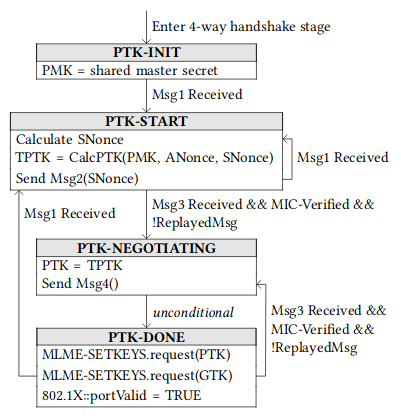
\includegraphics[scale=0.7]{images/wpa_state_machine.png}
    \caption{Esquema de ataque a la PTK y máquina de estados de la actualización de la PTK}
\end{figure}

Debido a que no todos los sistemas implementan del mismo modo WPA/WPA2, existen dos variantes de este ataque según en qué condición se acepte el tercer mensaje retransmitido. En caso en que se acepte la retransmisión de dicho mensaje en texto en claro, el ataque transcurre tal cual se lo describió anteriormente sin mayor dificultad. En cambio, en el caso de este solo se acepte siendo encriptado por la TK se tendrá que tener ciertos recaudos, por lo cual el mecanismo de ataque sufre ligeros cambios. Para esta versión del ataque los mensajes uno y dos son propagados sin ninguna intervención al igual que en la versión anterior, pero por el contrario el mensaje 3 es retenido. El atacante espera a que el \textit{Authenticator} al no recibir el mensaje 4, reenvíe el mensaje 3, con lo cual el atacante tendrá en su poder dos de estos terceros mensajes. Tras esto ambos mensajes son enviados al \textit{Supplicant} uno inmediatamente después del otro, con el objetivo de abusar de una situación de carrera que ocurre debido a que el controlador de red del atacante recibe y reenvía ambos mensajes al CPU principal antes de que este último le ordene enviar el mensaje 4 e instalar la nueva PTK y GTK. En consecuencia, ambos terceros mensajes son encolados en la cola de la CPU y procesados uno individualmente del otro, haciendo que el controlador instale la misma PTK y GTK dos veces. En particular si el dispositivo acepta la retransmisión del tercer mensaje sin encriptar esta versión del ataque ocurre como se lo acaba de describir, en cambio sí solo acepta la retransmisión del tercer mensaje estando este encriptado tras la instalación de la PSK, el mecanismo deberá realizarse en un \textit{4-way handshake} posterior al inicial. Si bien en este último caso se requiere que dicho mensaje se encuentre encriptado, esta no necesariamente debe ser encriptada mediante la última TK instalada, sino que acepta también la utilización de una TK predecesora. Esto suele ocurrir en versiones no muy recientes de OpenBSD, OS X, y MacOS.

\begin{figure}[H]
\centerline{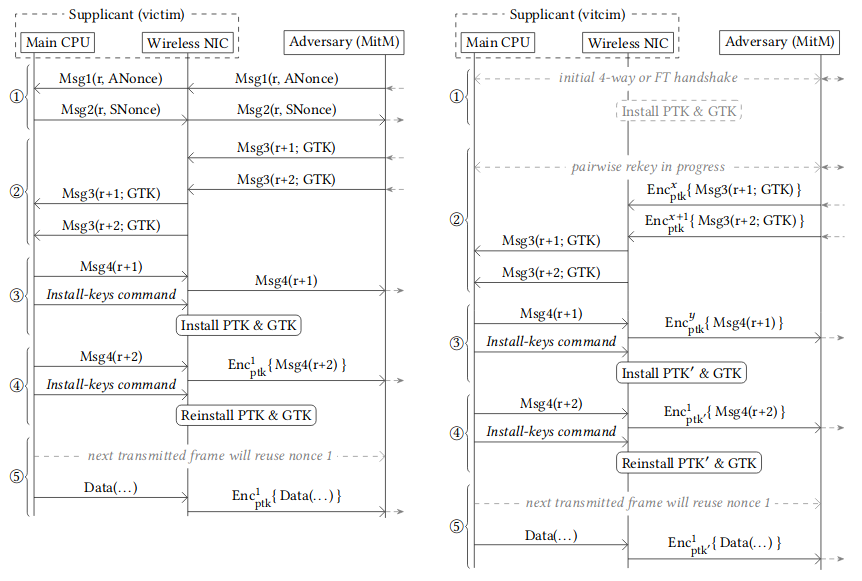
\includegraphics[scale=0.7]{images/krack_reinstalation_nonce.png}}
\caption{Ataque cuando el Supplicant aún acepta el Msg3 en texto en claro (izquierda), y cuando solo lo acepta encriptado (derecha)}
\end{figure}

Como ya hemos mencionado no todos los sistemas implementan de la misma forma WPA/WPA2, y este factor varía el impacto de este ataque de tal forma que, en algunas versiones de sistemas como Linux y Android, la retransmisión del tercer mensaje del \textit{4-way handshake} desencadena la instalación de una TK de todos ceros, de manera que el atacante apenas efectuado el ataque ya conoce la TK con la que se encriptan los mensajes. Esto parecería deberse a que el estándar sugiere como precaución a un posible robo interno de clave por parte de algún \textit{malware}, limpiar la TK en memoria una vez esta haya sido instalada. Por el contrario, algunas otras versiones de algunas plataformas como iOS y Windows, debido a que no implementan WPA/WPA2 tal cual como se indica en el estándar, en particular no aceptan el reenvío del tercer mensaje \textit{4-way handshake}, el ataque de reinstalación de PSK y GTK no es exitoso.




%En particular de entre estos ataques explicaremos como atacar el \textit{4-way handshake} tanto cuando el \textit{Supplicant} acepta la retransmisión del tercer mensaje en texto en claro, como si solo lo acepta encriptado. También expondremos como atacar el \textit{group key handshake} mediante un ataque de \textit{replay}.
\subsubsection{Deauthentication Attack}

Esta técnica consiste en realizar un ataque de \textit{Denial of Service} (DoS) forzando la deautenticación de los usuarios de una o varias redes por medio de la propagación de paquetes 802.11 de deautenticación. Como hemos visto anteriormente 802.11 requiere una etapa de autenticación y asociación a la hora conseguir acceso a una red para lo que implementa paquetes de autenticación y de asociación. Sin embargo, debido ciertas situaciones, como por ejemplo que la etapa de asociación no haya sido completada satisfactoriamente, o que haya habido un \textit{time out} asociado a algún \textit{handshake} de encriptación, es que además se incorporaron los paquetes de deautenticación y deasociación, con el código de tipo 1100 y 1010 respectivamente. Estos se propagan entre las estaciones y los \textit{access point} de la red con el objetivo de informar que se debe volver a un estado en el que la estación en caso de necesitar el acceso deberá realizar la etapa de autenticación o deautenticación respectivamente por alguna razón informada de acuerdo a un código especifico, y almacenado en el cuerpo de estos paquetes.

\begin{figure}[H]
\centerline{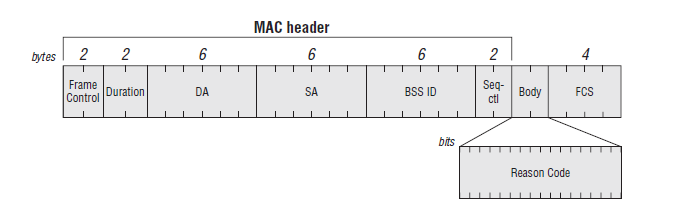
\includegraphics[scale=0.8]{images/deauthentication_frame.png}}
\caption{}
\end{figure}

Debido a que en el clásico 802.11 este tipo de paquetes a diferencia de los paquetes de datos no son encriptados o autenticados por ninguna clave secreta, se carece de mecanismo para verificar si un paquete de deautenticación fue enviado por quien dice ser en el campo origen. En consecuencia, los ataque de deautenticación toman ventaja de esto propagando continuamente a los \textit{access point} de cierta red objetivo paquetes de solicitud de deautenticación mediante \textit{spoofing}, es decir modificando los campos de origen para simular que este envío viene de parte de cierta estación. En consecuencia, el \textit{access point} intercambiara un paquete de notificación de la deautenticación, haciendo que la estación víctima se encuentre en una etapa en la que los paquetes de datos enviados a la red ya no sean aceptados hasta que se vuelva a realizar la etapa de autenticación y asociación. Ya que las direcciones de origen y destino en la capa de MAC no son encriptadas, es fácil en base a un \textit{sniffer} y un análisis posterior conocer cuáles son las direcciones MAC de las estaciones involucradas, necesarias para este tipo de ataques.

\begin{figure}[ht]
    \hspace{30px}
    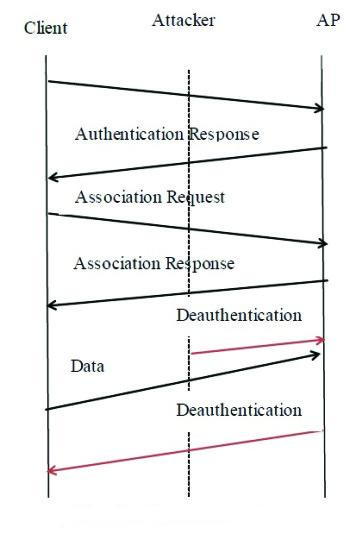
\includegraphics[scale=0.4]{images/deauthentication_attack.jpg}
    \hspace{40px}
    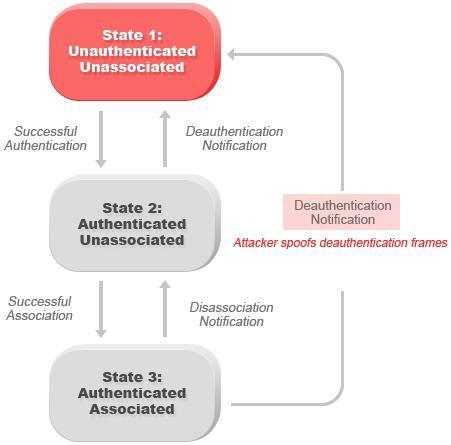
\includegraphics[scale=0.9]{images/deauthentication_process.jpg}
    %\caption{Encriptación por medio de WPA-TKIP y WPA2-CCMP}
\end{figure}

\subsubsection{Evil Twin}

Esta técnica tiene como objetivo lograr adoptar una posición MiTM por medio de un ataque de ingeniería social. Consiste en montar un \textit{Rogue AP} que imita el \textit{access point} de una red cuyo nombre ya es conocido, haciéndole cree a los potenciales usuarios que la red del atacante es la red anteriormente conocida. Dado que las BSSID que identifican los nombres de las redes son transportados sin encriptar en lo paquetes de \textit{beacon} propagados periódicamente, es sencillo mediante un \textit{sniffer} conocer dicho dato. Este ataque suele combinarse junto con un ataque de DoS como el  \textit{Authentication Attack}, por el cual los usuarios son deautenticados obligándolos a volver a conectarse en caso de que quieran seguir teniendo acceso a la red. En este paso los usuarios podrán observar dos redes con el mismo nombre y detectar el ataque, pero si no son suficientemente prudentes, podrán llegar a conectarse a la red del atacante sin darse cuenta. En algunas versiones de este tipo de ataque se le suele pedir la contraseña de la red por medio de alguna página especialmente diseñada para concordar con la red a la que se están conectado, cuando en realidad se trata de una técnica de \textit{phishing} para conseguir la contraseña de la red atacada. En otros casos debido a que los usuarios solo suelen conectarse para disponer de acceso a internet, se le disponer a la red del atacante de conexión a internet para así poder efectuar en su posición de MiTM otros ataques como SSLStrip o SSLSplit en orden de robar información sensible o credenciales.

\begin{figure}[H]
\centerline{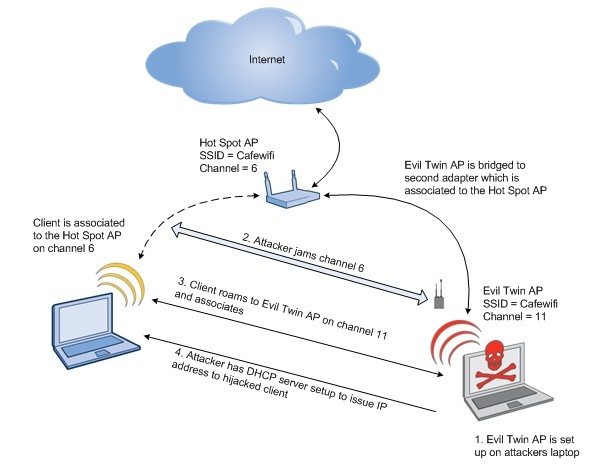
\includegraphics[scale=0.5]{images/evil_twin_attack.jpg}}
\caption{Ataque de Evil Twin}
\end{figure}

\subsubsection{ARP Spoofing}

Esta es una técnica de MiTM que consiste en invadir la red local con paquetes ARP de tipo Is-At. Estos paquetes sirven para informar que determinada dirección IP se encuentra asignada localmente a cierta dirección MAC, y son enviados con dirección \textit{broadcast} con el objetivo de que todos los nodos de la red actualicen su tabla ARP de manera acorde a la información transferida por dicho paquete. La técnica de \textit{ARP Spoofing} abusa del hecho de que no existe a priori métodos de seguridad que aseguren que la información provista por estos paquetes es legitima. El ataque consiste en inundar la red con estos paquetes conteniendo información falsa, en particular indicando que la IP asignada al equipo víctima corresponde a la dirección MAC del equipo del atacante, haciendo que todo aquel que quiera comunicarse luego con la víctima, envié la información erróneamente al equipo de la víctima. Para esto el atacante además habilita la opción de \textit{IP forwarding} para poder reenviar los paquetes destinados a la víctima (que tras el ataque llegan a él) hacia la correcta dirección MAC de la víctima, de manera hacer transparente la intrusión. 

\begin{figure}[H]
\centerline{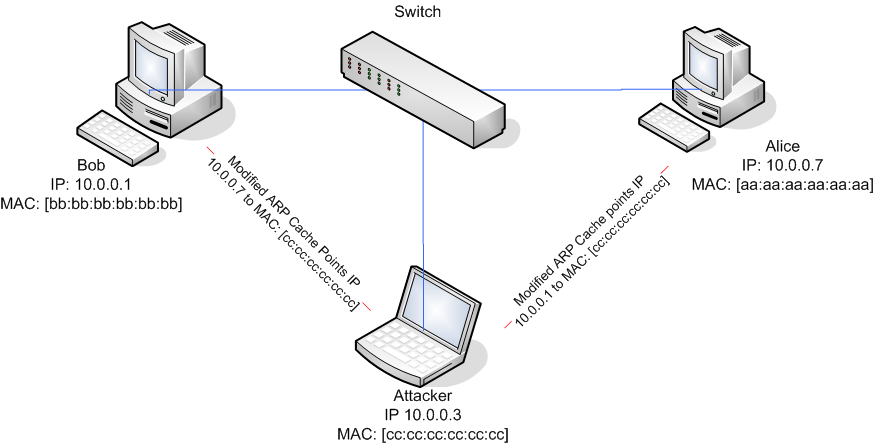
\includegraphics[scale=0.4]{images/arp_spoofing.png}}
\caption{ARP Spoofing}
\end{figure}

\subsubsection{SSLStrip}

Esta técnica fue propuesta en 2009 por Moxie Marlinspike con el fin de demostrar las vulnerabilidades generadas por prácticas no seguras como las que resultan en la vulnerabilidad de \textit{Mixed Content}. Esta vulnerabilidad se presenta cuando una misma página no se asegura de invocar recursos utilizando siempre HTTPS, si no que por la mezcla de invocaciones tanto mediante HTTPS como HTTP. Al acceder a una página normalmente se solicita un recurso HTML el cual es el cuerpo de la página propiamente dicho, no obstante, usualmente este no contiene todo el contenido de la página, sino que en base a este archivo principal se generan otras invocaciones a otros recursos que componen la página. Por alguna razón existen muchas páginas que permiten acceder a ellas mediante HTTP, y luego utilizan HTTPS para invocar ciertos recursos específicos. Bajo estas condiciones y mediante una situación de MiTM, SSLStrip permite realizar lo que se conoce como un \textit{downgrade attack} es decir forzar el uso de protocolos o medidas más pobres de seguridad. Para esto trabaja interceptando el paquete de respuesta HTTP que contiene el HTML principal, para luego identificar y modificar todas las URIs que se accedan mediante HTTPS, de modo que hagan uso de HTTP. Debido a que HTTP por sí solo no encripta los campos enviados, toda la información intercambiada es visible para cualquiera que pueda interceptarla. a causa de que muchos usuarios a veces no suelen tomar el recaudo de verificar si se está accediendo vía HTTPS, y, lo que es más, simplemente acceden mediante el \textit{browser} sin especificar el protocolo a utilizar, algunos servidores web suelen responder al pedido con una redirección al mismo sitio, pero utilizando HTTPS. Si bien esto podría asegurar la conexión si la redirección se concreta correctamente, SSLStrip se encarga de lo contrario. Dado que se está en una posición de MiTM, el atacante puede interceptar la redirección y modificarla para que refiera al sitio con HTTP, para luego capturar la posterior consulta que esta genera. A su vez el atacante se conecta por HTTPS al servidor por medio de la redirección original, haciéndole creer al servidor que se está manteniendo una conexión segura con el usuario legítimo, mientras que en realidad el atacante estará reenviando el contenido recibido en HTTPS hacia la victima por medio de HTTP. De esta manera todos los datos enviados por este se transmitirán hacia el atacante sin ser cifrados por HTTPS, y por ende ser leídos abiertamente, y así entre cosas permitiendo robar datos sensibles, como credenciales, o simplemente monitorear transparentemente el uso del sitio por parte de la víctima.

\begin{figure}[H]
\centerline{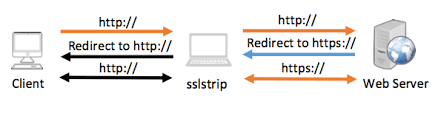
\includegraphics[scale=0.8]{images/sslstrip_redirect.png}}
\caption{}
\end{figure}

%\pagebreak

\subsubsection{SSLStrip2}

Con el objetivo de prevenir ciertos ataques como el de SSLStrip previamente descritos, se inventó un nuevo mecanismo llamado \textit{HTTP Strict Transport Security} (HSTS). La idea detrás de este nuevo mecanismo a configurar el \textit{browser} para que al acceder a ciertas URLs lo hagan por medio del protocolo HTTPS. Para ello al conectarse a al servidor web por medio de HTTP, este lo redirigirá indicando además en un campo especifico en el \textit{header} HTTP que se quiere utilizar la política de HSTS. Si el \textit{browser} soporta HSTS, al observar dicho campo especifico, almacenará esa URL en una caché especialmente dedicada, junto con algunos otros datos como el tiempo de vida de dicha entrada en la caché. A la hora de acceder a algún sitio, el \textit{browser} buscará en dicha caché si hay alguna entrada que corresponde a la URL ingresada, si es así modificada la URL ingresada para que esta acceda mediante HTTPS. De por si este mecanismo no es completamente seguro, ya que si el atacante intercepta la respuesta del servidor en la que viaja el header con el campo de HSTS, puede modificarlo de manera que luzca como una respuesta HTTP clásica, y así evitar su almacenamiento en la caché HSTS. Nótese que esto último podría ocurrir tanto la primera vez que la víctima se visita el sitio, como también en el caso de que se conecte por primera vez a él tras caducar el tiempo de vida de la entrada correspondiente en la caché. Si bien estas ventanas de tiempo vulnerable siguen existiendo, el mecanismo HSTS supone un obstáculo no despreciable a la hora de intentar un ataque SSLStrip.

Debido a que con este mecanismo el acceso a las URL en la caché se realiza desde el principio por medio de HTTPS, SSLStrip no tiene manera de interceptar el intercambio antes de que se establezca la conexión HTTPS, y por ende el ataque falla. En orden de sortear este obstáculo, el investigador Leonardo Nve publicó en base al clásico SSLStrip una versión superadora, capaz de burlar HSTS. Esta nueva versión fue bautizada como SSLStrip2 o SSLStrip+, y consiste en engañar a la víctima haciéndole creer que cierta IP que resulta de la traducción del dominio por medio de los DNS, es en efecto la IP del dominio al que se intenta acceder, cuando en realidad corresponde a otro dominio predefinido por el atacante. Para esto el atacante intercepta las consultas DNS que típicamente viajan mediante UDP, y comprueba si corresponde a algún sitio del cual le interesa interceptar el tráfico, si no es así simplemente resuelve la consulta mediante un DNS legítimo y se la devuelve a la víctima, en caso contrario lo que devuelve es una respuesta DNS falsa, indicando que corresponde a la IP de otro dominio, el cual suele mantener un nombre muy similar, con el objetivo de no levantar sospechas del lado del cliente. De esta forma como el nombre del dominio es distinto, y por ende también lo es su URL, el \textit{browser} no encontrará ninguna entrada en su caché HSTS, y permitirá el uso de HTTP, volviendo a la misma situación favorable en la que funciona el clásico SSLStrip.

\subsubsection{SSLSplit}

Esta es una técnica y herramienta de MITM licenciada por Daniel Roethlisberger que permite vulnerar conexiones encriptadas por medio SSL/TSL. A diferencia de otras técnicas como SSLStrip, esta permite el acceso libre al tráfico de la víctima sin que esta deje de mantener una conexión SSL/TSL con el supuesto servidor web. Normalmente las conexiones SSL suelen mitigar los fallos de seguridad a la confidencialidad por técnicas de MiTM mediante el uso y validación de certificados. No obstante, SSLSplit logra generar certificados dinámicamente que el equipo de la víctima considera como válidos, y de los cuales se conoce su clave privada. Este último punto es una cuestión no trivial, ya que solo se aceptarán certificados que hayan sido firmados por alguna entidad certificante en la que se tenga confianza, y debido a que generalmente es computacionalmente imposible deducir en un tiempo razonable la clave privada utilizada por dichas entidades, SSLSplit debe recurrir a cierto arsenal especial de contramedidas.

Existen varias técnicas que pueden llegar funcionar bajo ciertas condiciones para engañar a la víctima y hacerle creer que el certificado presentado es de quien dice ser. Una posibilidad es agregar un nuevo certificado auto firmado de una nueva autoridad certificante (que el atacante controle) a la lista de certificados de confianza de la víctima. De esta forma SSLSplit podrá generar al vuelo certificados firmados por esa autoridad certificante en quien ahora la victima confía. Debido a que para este método es necesario tener acceso al equipo objetivo durante al menos cierto periodo de tiempo y bajo ciertos niveles de permisos, esta opción suele no estar disponible. 

Otras alternativas están relacionadas con el uso de un certificado legítimamente emitido por una autoridad certificante en el la victima confía, pero con el inconveniente de que su periodo de validación expiró, y cuya clave privada es conocida. Para esto el atacante deberá poder interceptar y modificar abiertamente las comunicaciones de OCPS, de forma de que la víctima no llegue a comprobar que el certificado ya no es válido.

%Entre     esta manera por más que se tenga el recaudo de comprobar que se está usando SSL/TSL, la conexión podría estar siendo intervenida y desencriptada. SSLStrip en base a una posición de MiTM, engaña a la víctima haciéndole creer que se está conectando con el servidor legítimo, cuando en realidad se está conectando al equipo del atacante. 

%Para validar que las claves publicas utilizadas son efectivamente del dominio al cual se pretende acceder, se hace uso de certificados firmados por autoridades certificantes. De esta manera antes de aceptar cualquier certificado como valido, se comprueba que el nombre del dominio al que refiere sea el mismo, y se comprueba que el certificado haya sido emitido por una entidad certificante confiable. Para esto hace uso de certificados previamente instalados que dan fe de los
\begin{figure}[H]
\centerline{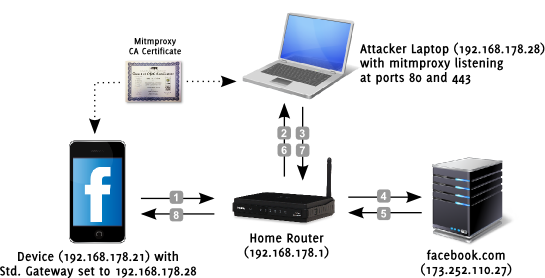
\includegraphics[scale=0.8]{images/sslsplit_diagram.png}}
\caption{}
\end{figure}

%\pagebreak

\section{Experimentación}

\subsection{Metodología}

\subsubsection{Rogue AP}

\begin{figure}[H]
\centerline{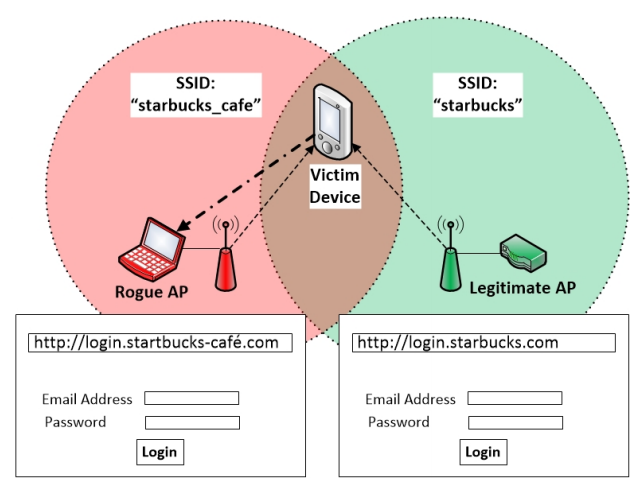
\includegraphics[scale=0.6]{images/rogue_ap.png}}
\caption{Esquema de un Rogue AP}
\end{figure}

Con el objetivo de analizar el tráfico de red generado por el uso de distintos positivos conectados a internet, simulamos ser un potencial atacante el cual logro obtener una posición de MiTM con respecto a la conexión de dichos dispositivos. Para esto levantamos un \textit{Rogue Access Point} (Rogue AP) con la idea de simular la conexión a ella por algún método ilegitimo, como por medio de la técnica de \textit{Evil Twin}. Este Rogue AP fue implementado mediante una \textit{notebook} a la cual se le conecto una placa de red externa con el objetivo de tener otra interfaz extra (además de la placa interna), de manera que por una interfaz pudiéramos montar el \textit{access point} propiamente dicho, y por la otra pudiéramos conectarnos a otra red por la cual dispusiéramos de acceso a internet. En el caso de Linux esto se logró mediante una herramienta conocida como \textit{Hostapd} que provee el servicio de \textit{access point} virtual y el sistema de autenticación. Para controlar los servicios de DNS y DHCP que acompañan este procedimiento utilizamos además el servicio de \textit{Dnsmasq}. En el caso de Windows esto lo logramos de manera más directa con otra herramienta llamada Netsh, aunque nos requirió usar ciertos \textit{drivers} compatibles.

%Para el caso de la experimentación de ataques como SSLStrip y SSLSplit utilizamos \textit{Burp}. 
%%%
%Con el objetivo de poder observar el tráfico de la red, poder analizar malas implementaciones de apps o ataques, realizamos lo que se conoce como Rouge Ap denominado de esta manera dado que nos brinda la posibilidad de inspeccionar todo en tráfico que se genera en la red para poder analizar y atacar.

%Para esto utilizamos una herramienta que es netsh (Windows 10) que nos permite crear una access point en base a una placa wifi o ethernet. Dicha herramienta genera otra conexión wifi disponible creando una placa virtual y compartiendo internet (técnica denominada internet sharing) con una interface real, de esta forma, los usuarios se conectan a esta conexión nueva generada y esto nos permite manejar todo el tráfico que pasa por la misma.

%No todos los drivers de placas wifi soportan esta tecnología, para realizar esto tuvimos que buscar una versión del driver de la placa wifi que lo tuviese activado.

En el caso de Netsh para verificar que la interfaz que utilizamos esté disponible, lo hacemos por medio del comando \textbf{netsh wlan show drivers} de la cual luego podremos verificar que la opción denominada \textbf{hosted network support} esté activada.

\begin{figure}[H]
\centerline{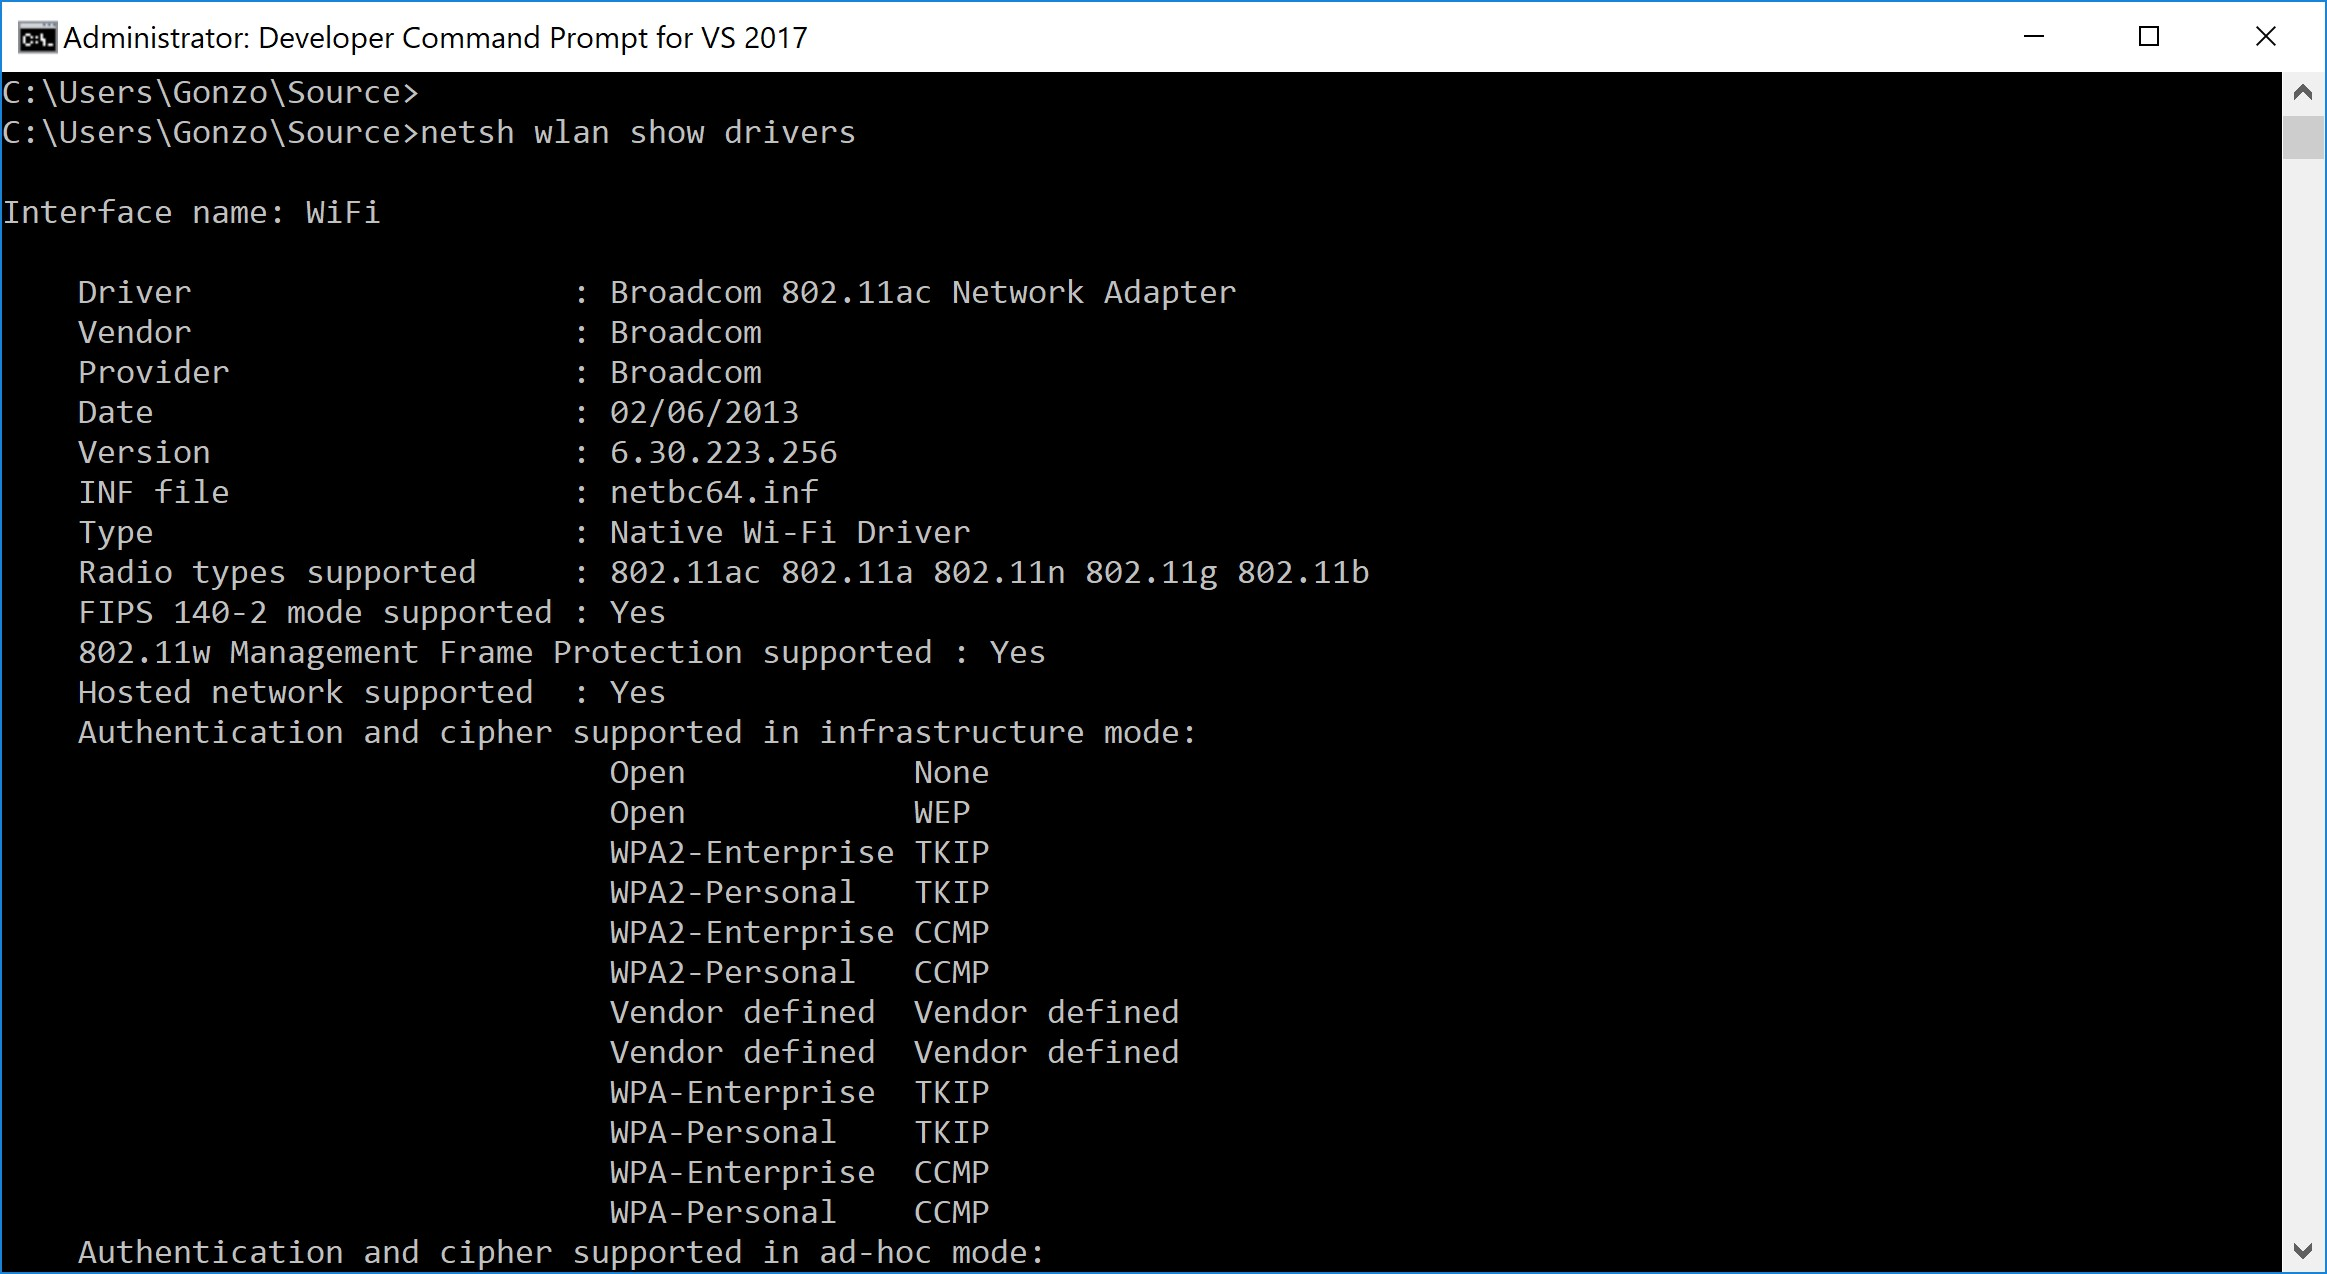
\includegraphics[scale=0.2]{images/hosted_network.jpg}}
\caption{}
\end{figure}

Luego, podremos crear la placa virtual con el siguiente comando:

\textbf{netsh wlan set hostednetwork mode=allow ssid=(nombre de red) key=(contraseña)}

Al terminar el proceso de creación podremos observar que tenemos una nueva placa wifi (virtual) con el nombre ingresado en el parámetro \textit{ssid}. Con esto ya podremos iniciar y detener el servicio respectivamente con los siguientes comandos:

\textbf{netsh wlan start hostednetwork}

\textbf{netsh wlan stop hostednetwork}

Para finalizar ya que necesitamos que nuestro \textit{Rogue AP} disponga de conexión a internet, en el menú de manejo de placas de red, botón secundario sobre la placa física, solapa compartir y seleccionamos la opción compartir con la placa virtual creada.

%Para finalizar, basta compartir internet de la placa real con la virtual para poder usar el ap nuevo, como uno más.

%Para eso vamos al manejo de placas de red, botón secundario sobre la placa física, solapa compartir y seleccionamos la opción compartir con la placa virtual creada.

\begin{figure}[H]
\centerline{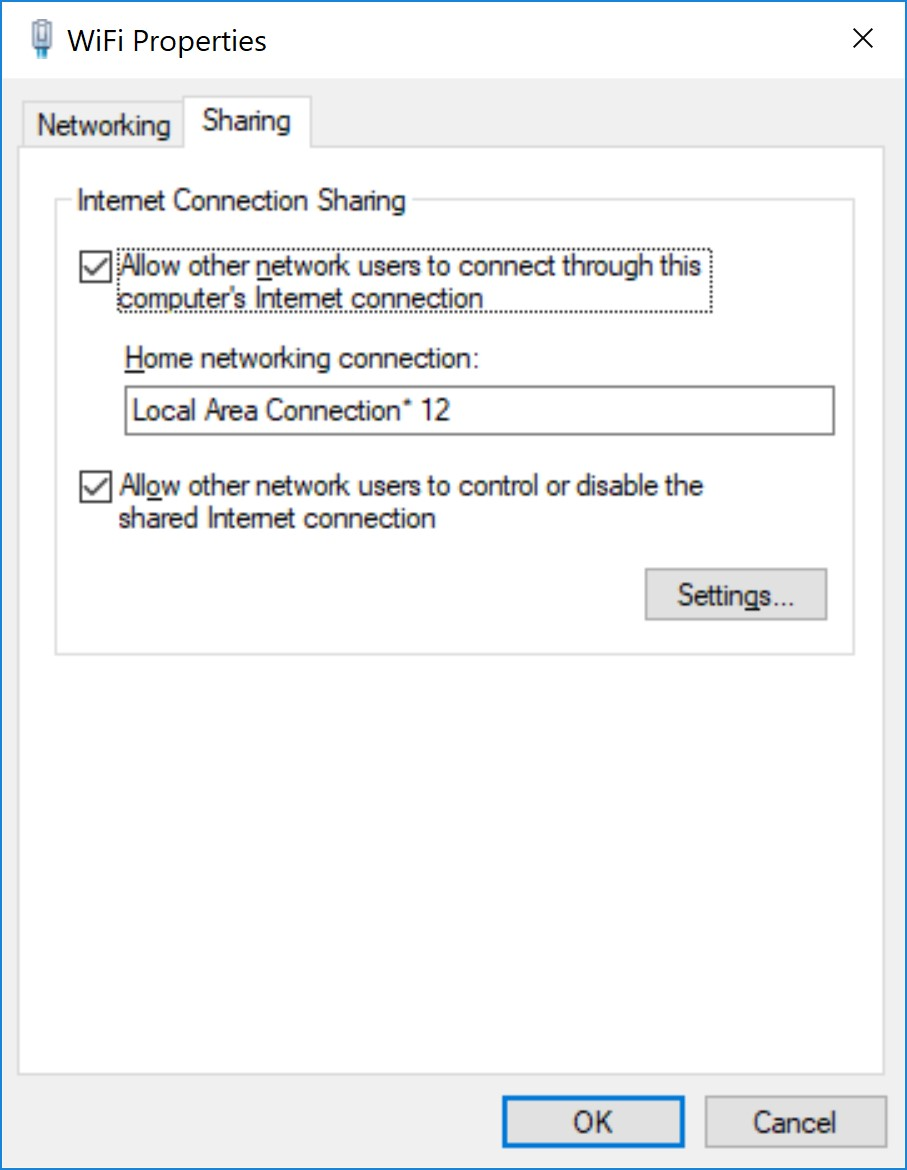
\includegraphics[scale=0.2]{images/internet_sharing.jpg}}
\caption{}
\end{figure}

Una vez terminado esto, ya podemos ver y usar nuestro Rogue AP como un \textit{access point} cotidiano que provee servicio de conexión a internet. En nuestro caso la red creada se llama TpSegInf, pero en un escenario de ataque más serio podríamos haberla llamado de acuerdo a un nombre engañoso, como \textit{MacDonald-Free} para hacer creer a alguien en búsqueda de acceso a internet que se trata de una red gratuita de la respectiva empresa. O también podríamos haberla llamado TeleCentro-66b6-2.4G, en orden de engañar a los típicos usuarios de dicha red que nos aparece en el nuestro rango.

\begin{figure}[H]
\centerline{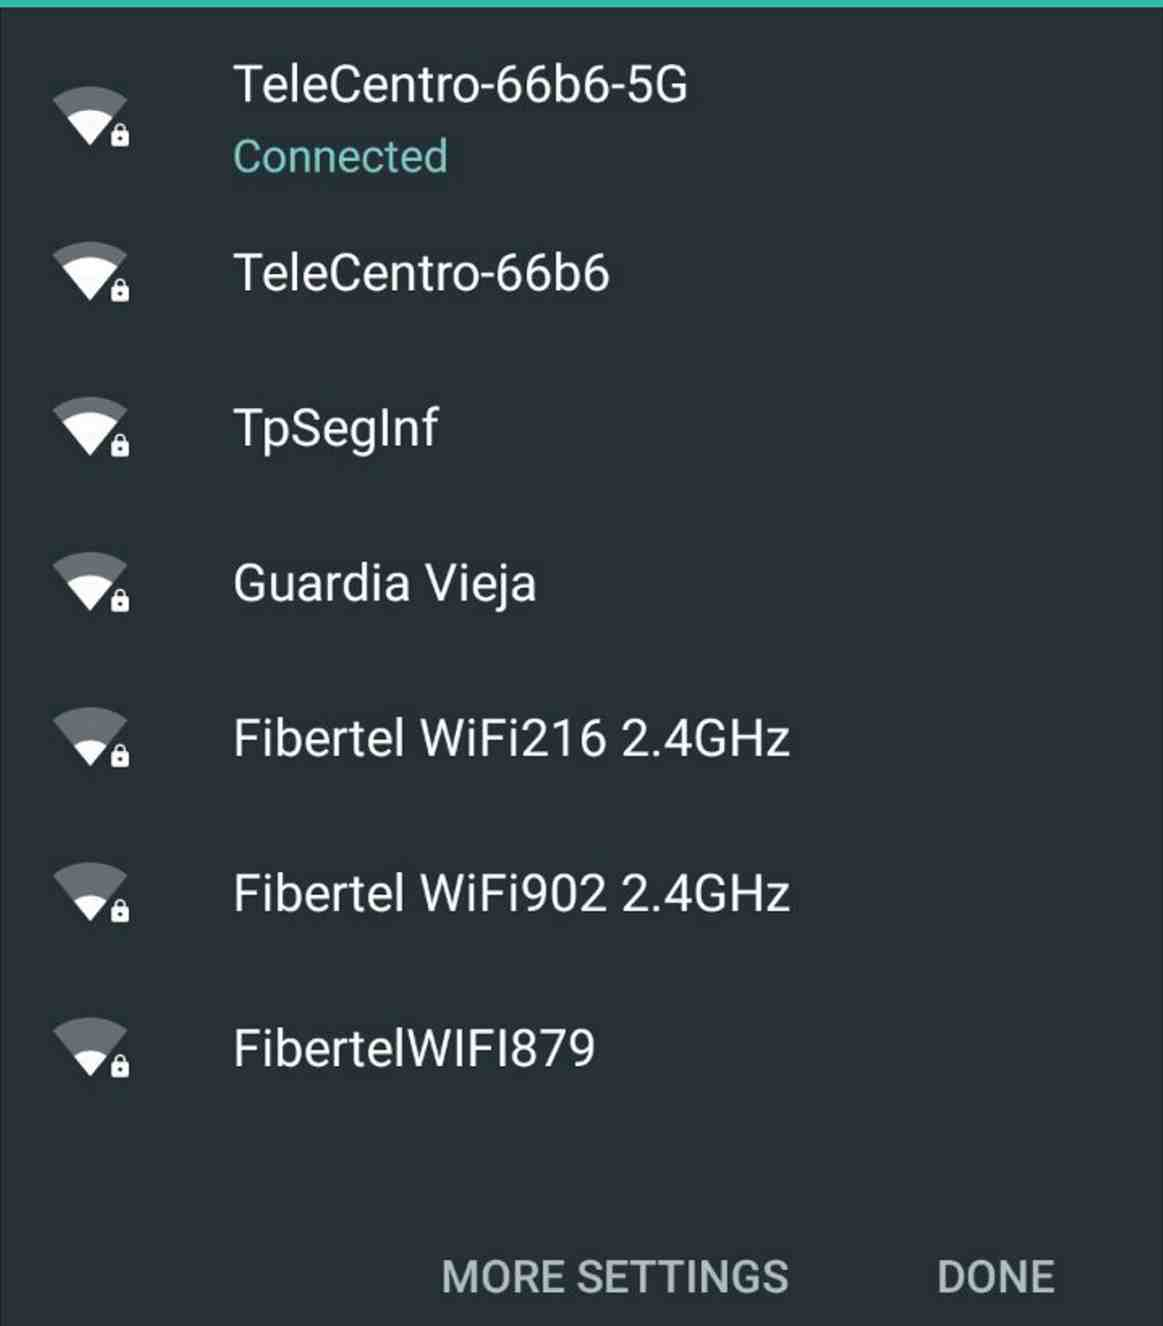
\includegraphics[scale=0.2]{images/rougeap.jpg}}
\caption{}
\end{figure}

%\pagebreak
\subsubsection{Herramientas de análisis}

A la hora de analizar la seguridad de ciertas aplicaciones y servicios analizamos por un lado un análisis pasivo del tráfico con el objetivo de identificar posibles vulnerabilidades en la forma de trabajar de estos. Estando en la posición de MiTM que nuestro Rogue AP nos ofrecía, utilizamos una popular herramienta de captura de paquetes llamada \textit{Wireshark}, la cual nos ayudó a identificar aquellos paquetes que viajan en protocolos no seguros como HTTP, para luego estudiar si se utilizaba algún método de encriptación por capa de aplicación o si simplemente como en muchos casos analizados viajaban en texto plano. En el caso de los \textit{smartphones} para comprobar que el mismo tráfico llegaba y salía desde él era el mismo capturado por el Rogue AP utilizamos otras herramientas de captura de tráfico que corrían localmente en los dispositivos móviles analizados, como por ejemplo \textit{tPacketCapture}.

A la hora de experimentar sobre la aplicación de ciertos ataques investigamos previamente sobre distintos \textit{frameworks} que podían llegar a sernos de utilidad a la hora de efectuar estos mecanismos. Entre ellos destacamos \textit{Ettercap}, \textit{Bettercap}, y \textit{Burp Suite}, aunque existen muchas otras. En particular expondremos ciertos resultados de ataques utilizando ésta última.

Burp Suite es una herramienta para \textit{testing} de aplicaciones que hacen uso de conexión a internet por medio de alguna red. Esta no solamente nos permite analizar tráfico, sino que además nos ofrece un extenso catálogo de herramientas que podemos aplicar sobre las conexiones establecidas a través del punto de acceso configurado. Entre los mecanismos ofrecidos experimentamos con ella los ataques previamente explicados de \textit{SSLStrip} y \textit{SSLSplit}.

%(como ataques, que se encuentran dentro de la solapa Intruder). Vamos a usar de esta herramienta especialmente dos opciones Converts https links to http y Match and Replace.\newline\newline
%Converts https links to http realiza el denominado ataque \textit{ssltrip}, esto es, una vez que un usuario o sistema realiza un get que pasa por Burp, el mismo captura la respuesta y de manera automática, cambia todos los links https por http, enviando esa respuesta el cliente. De esta forma, se evade casi invisiblemente para el usuario, la seguridad del certificado de la página, dado que si bien el request original quizás si fue https, en el cuerpo de la respuesta todos los links fueron cambiados para no tener certificado. \newline\newline
%Match and replace, esta opción tiene muchas utilidades posibles, es usada para reemplazar automáticamente partes del request o del response del mensaje http (o https). Podemos definir varias reglas de manera independiente (para request, response, header, body, etc), y cada regla puede especificar un string como literal o una expresión regular para buscar y reemplazar en la opción seleccionada. Para cabeceras de mensajes donde la condición de búsqueda es la cabecera entera y el reemplazo en vacío, entonces el mensaje es eliminado.

%A la hora de experimentar sobre la aplicación de ciertos ataques investigamos sobre distintos \textit{frameworks} que podían llegar a sernos de utilidad a la hora de efectuar estos mecanismos. Entre ellos destacamos \textit{Ettercap}, \textit{Bettercap}, y \textit{Burp}, aunque existen muchas otras. 
\pagebreak
 
\subsection{Aplicaciones Android}

\subsubsection{BA Cómo Llego}

\begin{figure}[ht]       
    \fbox{
\includegraphics[scale=0.6]{images/como_llego_logo.png}}   
    \hspace{38px}
    \fbox{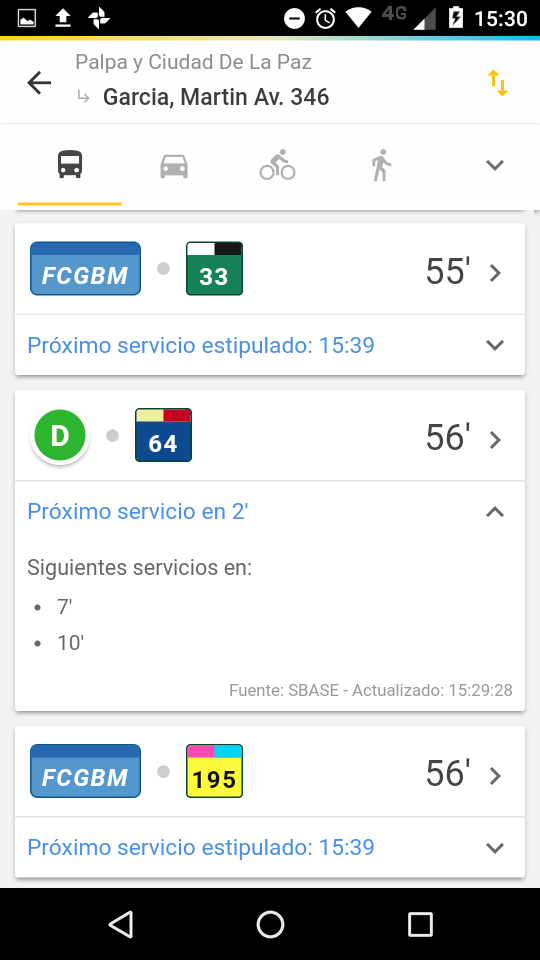
\includegraphics[scale=0.2]{images/como_llego_muestra1.png}}
    \hspace{38px}
    \fbox{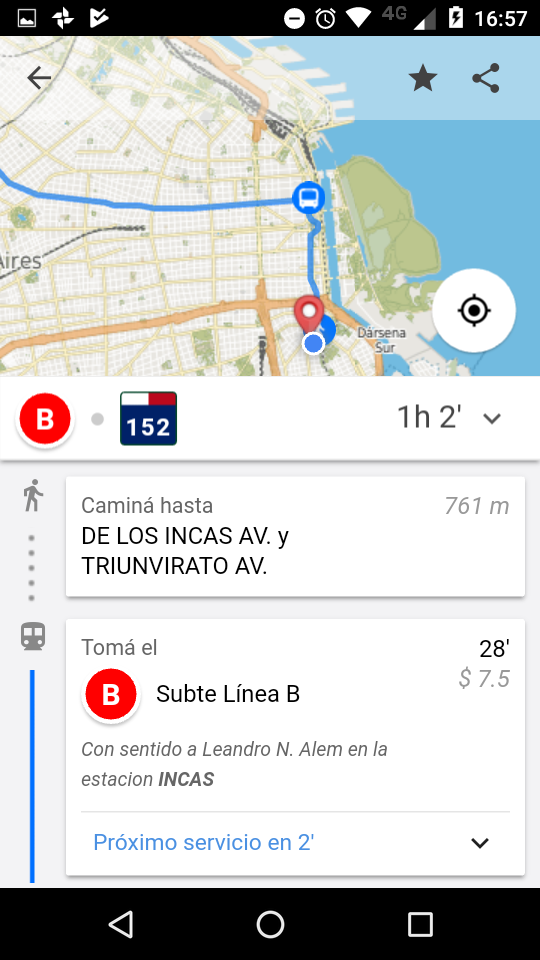
\includegraphics[scale=0.2]{images/como_llego_muestra2.png}}
    \caption{App de como llego}
\end{figure}

Esta es una aplicación de Android provista por el gobierno de la ciudad para facilitar la búsqueda de posibles recorridos y alternativas de transportes con el objetivo de encontrar de la forma más rápida la manera de llegar a un destino en particular determinado por el usuario. Para esto el usuario debe especificar el nombre de la calle, número de dirección y opcionalmente los métodos de transporte predilectos.

Con el objetivo de comprobar la seguridad en las consultas \textit{online} que esta podría llegar necesitar con cada solicitud del usuario hemos capturado el tráfico durante el uso de esta aplicación. Tras analizarlo con la herramienta de \textit{Wireshark} hemos comprobado que realizaron consultas hacia el dominio de \textit{ws.usig.buenosaires.gob.ar} por medio de HTTP sin hacer uso de protocolos de seguridad como SSL/TSL. Esto en consecuencia supone un riesgo importante al menos si se transporta información sensible, para comprobar esto analizamos el contenido de los consultas y respuestas generadas. De este análisis descubrimos que \textit{BA Como Llego} se basa a la hora de resolver la ubicación de una dirección solicitada, en un servicio de geo codificación que ofrece el \textit{ws.usig.buenosaires.gob.ar}. Con el cual interactúa en primer lugar solicitando la URI en la que viajan el código de calle y el número de la dirección sin ningún tipo de encriptación, por medio de los campos \textit{cod\_calle} y \textit{altura}.

\begin{figure}[H]
\centerline{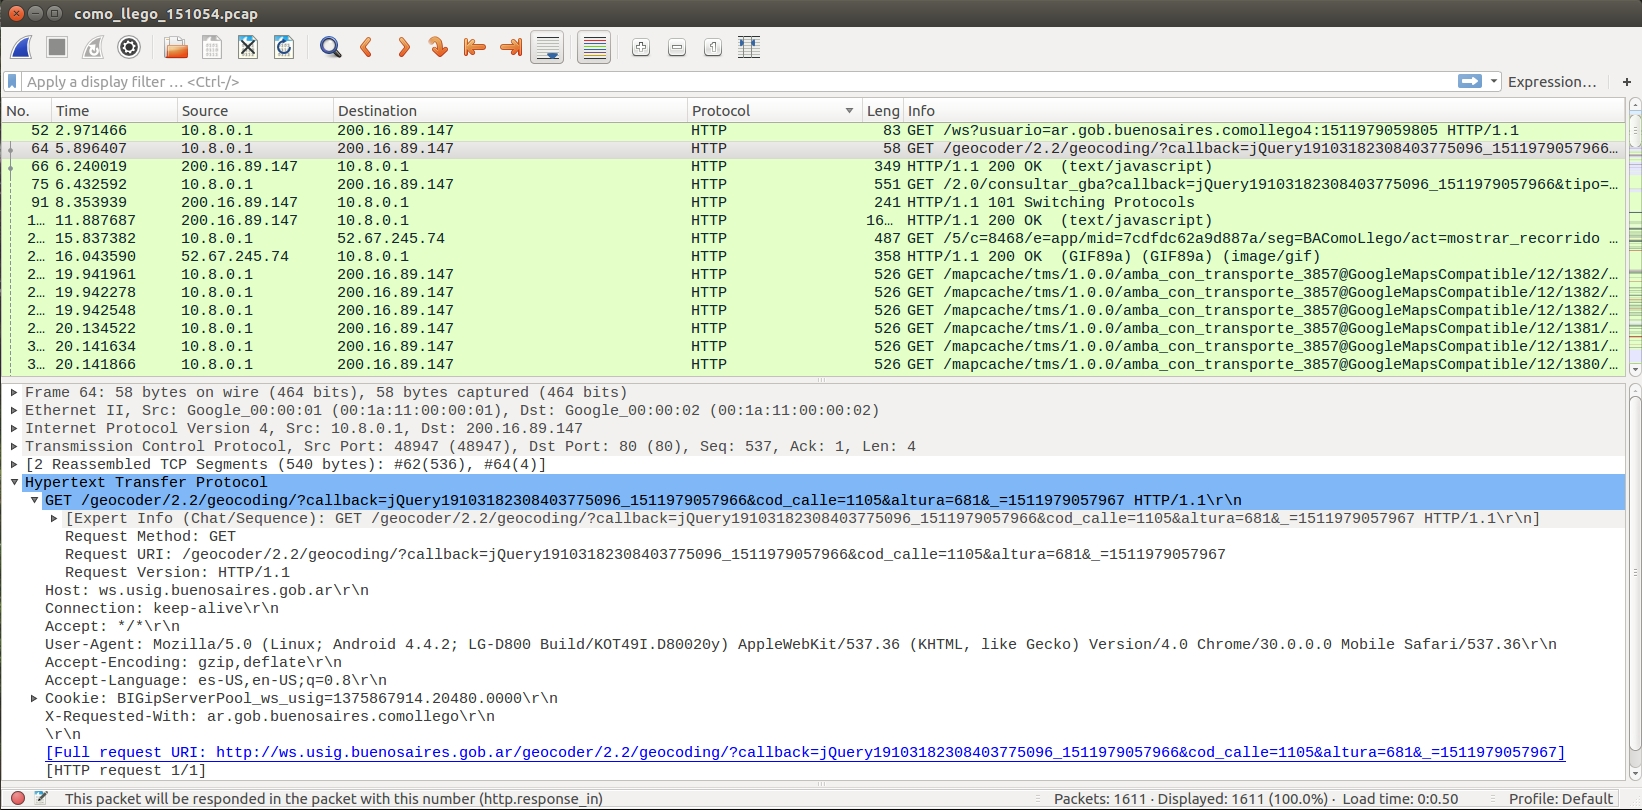
\includegraphics[scale=0.28]{images/como_llego_geocoder.jpg}}
\caption{}
\end{figure}

A su vez este servicio respondía entregando un par de coordenadas \textit{x} e \textit{y} asociadas a la dirección solicitada. Si bien estas coordenadas no correspondían a longitud y latitud, parecían ser análogos. Analizándolo desde el lugar de un posible atacante en situación de MiTM investigamos un poco el servicio de geolocalización de \textit{ws.usig.buenosaires.gob.ar} y nos percatamos que permitía convertir dichas coordenadas en una secuencia de datos que contenían los nombres de las calles entre las que queríamos llegar, el número de la dirección, y código postal entre otros. Mas concretamente para esto utilizamos el servicio provisto por \textit{ws.usig.buenosaires.gob.ar/geocoder/2.2/reversegeocoding?\textbf{x=101910.00695}}\&\textit{\textbf{y=102062.917733}}
 de geo codificación inversa. De esta forma como atacantes podemos conocer el nombre de la calle y dirección solicitadas por la víctima, y así conocer a donde posiblemente va a dirigirse. Si bien el servicio al brindar aquella información no expone de por sí solo datos propios de algún usuario, bajo el contexto de uso que la aplicación le da y en la manera que esta realiza la conexión, esta información adquiere otro significado, convirtiéndola en información sensible en cierto grado.

\begin{figure}[H]
\centerline{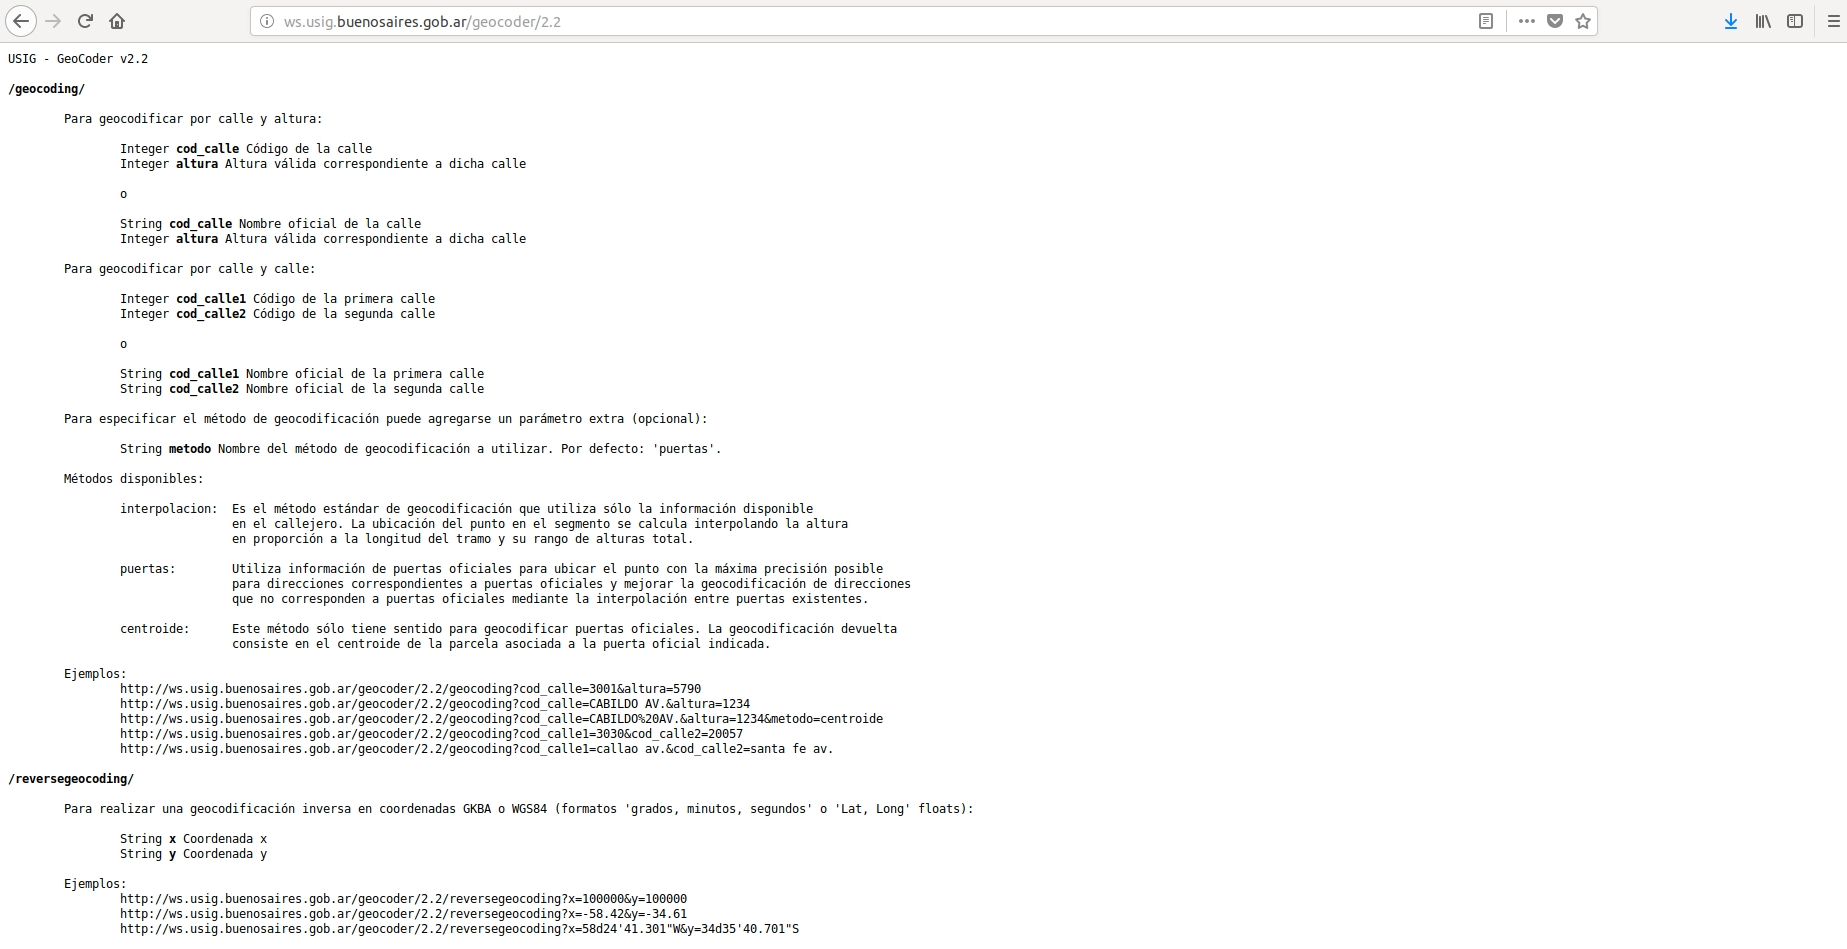
\includegraphics[scale=0.25]{images/ws_usig_buenosaires_v2.jpg}}
\caption{}
\end{figure}

Entre otras observaciones nos encontramos que \textit{BA Cómo Llego} no solo se conecta de manera insegura por medio de HTTP a la hora de resolver las coordenadas de una dirección, sino que también lo hace para otro tipo de datos, como por ejemplo las imágenes que componen a los mapas de la ciudad. De este modo un atacante en posición de MiTM podría modificar las URIs de los \textit{request} HTTP o directamente modificando los \textit{response} HTTP para engañar a la víctima mostrándole un mapa completamente diferente, o en general imágenes especificas elegidas por el atacante. La misma idea y aún más simple se podría llegar a lograr cambiando el código de calle y la altura en los \textit{request} de geo codificación, con el objetivo de engañar a la víctima para que vaya a alguna otra dirección.

Al principio pensamos que la baja seguridad que se le dio a la aplicación en este sentido se debía a que el servicio web de \textit{ws.usig.buenosaires.gob.ar} solo aceptaría conexiones HTTP sin TSL. Sin embargo, luego comprobamos que dicho dominio aceptaba también el uso de HTTPS, por lo que es ese sentido podría haberse diseñado una versión más segura de esta aplicación.

\subsubsection{Análisis general}

Como parte de nuestra experimentación hemos analizado el uso de la red que un \textit{smartphone} LG G2 D800 realizaba al mantenerse en reposo sin ser utilizado por ningún usuario, para esto dejamos conectado el dispositivo a un \textit{Rogue AP} el cual capturaba y despachaba todo el tráfico hacia y desde el dispositivo. Como esperábamos las comunicaciones por medio de dicha red no cesaron, hemos visto paquetes relacionados con servicios de mensajería como \textit{Gmail}, y otras de aplicaciones de redes sociales como \textit{Facebook}, en particular esta última nos llamó la atención debido a que si bien dicha aplicación se encontraba instalada en el dispositivo, nunca se la utilizo para acceder a ninguna cuenta con lo cual es llamativo el constante uso de la red que esta demanda.

Analizamos también el uso de la red durante el proceso de instalación de varias aplicaciones por medio de \textit{Play Store} en búsqueda de información enviada por medios no seguros. Sin embargo, nos encontramos con que todos los datos de las aplicaciones en descarga fueron enviados de manera segura por medio de TLS.

A su entre capturas realizadas con el fin de analizar cierto uso propio de cierta aplicación en uso, nos encontramos con ciertos envíos de datos sensibles relacionados con servicios de \textit{advertising}, asociados a dominios como por ejemplos \textit{ad-x.co.uk}, \textit{ads.mopub.com}, o \textit{ads.aerserv.com}. Estos servicios parecerían enviar regularmente información sensible por lo cual recolectamos datos como la versión del \textit{kernel}, marca y modelo del dispositivo, nombre de la empresa de telefonía asociada, y entre otros datos más sensibles se encontraba, la dirección MAC del equipo, el \textit{Unique Device ID} (UDID), y la longitud y latitud. Estos últimos datos de coordenadas nos llamaron mucho la atención, al principio pensamos que podrían llegar a ser coordenadas relacionadas a los servidores del servicio, pero al utilizar un GPS descubrimos que las coordenadas correspondían a un punto que se encontraba a media cuadra del sitio en donde se encontraba el dispositivo al momento de la captura del tráfico, el cual es un sitio residencial. Comprobamos además que la dirección MAC y UDID pertenecían al dispositivo analizado, lo cual delata una práctica insegura ya que estos identifican unívocamente al dispositivo, y no a una instalación en particular como suele recomendarse.


%mediante el uso de diferentes aplicaciones

\subsection{Sitios Web}

\subsubsection{Movistar}

Movistar ofrece en su sitio web \textit{movistar.com.ar} distintos servicios entre los cuales se encuentra su tienda \textit{online} en la cual nos permiten comprar por medio de tarjeta de crédito distintos equipos expuestos en su catálogo de venta. Otro servicio que proveen es la posible consulta \textit{online} de los datos de nuestra línea, entre los cuales se encuentran el saldo y facturas pagas o a pagar. Para acceder a ello el sitio nos solita realizar un proceso de registro mediante un correo electrónico, una contraseña, nombres, DNI, un código de validación por enviado a nuestro número telefónico mediante un SMS, entre otros datos. Esto no es de extrañarse debido a que los datos de la línea, y facturas asociadas no deberían ser información de libre acceso, por lo que los recaudos no están de más. No obstante, encontramos ciertas prácticas muy desaconsejadas que permiten a pesar de dichos recaudos apropiarse de la cuenta del usuario.

Para empezar \textit{movistar.com.ar} a día de hoy permite el uso tanto de HTTP y HTTPS, obligando a indicarlo explícitamente si se quiere acceder mediante este último debido al entrar por medio de \textit{movistar.com.ar} por defecto es interpretado como una solicitud de acceso por medio HTTP, y los servidores de Movistar ni siquiera realizan ningún tipo de redirección a la versión más segura. Sin embargo, al acceder por medio de otros enlaces a secciones como la tienda o la cuenta, estos obligatoriamente son forzados a trabajar por medio de HTTPS. Si bien estos enlaces secundarios usan una mayor seguridad, debido a que la página principal puede trabajar por medio de solo HTTP, esta situación de \textit{mixed content} se ofrece de manera ideal a un ataque de SSLStrip como ya hemos explicado anteriormente.

Desgraciadamente los inconvenientes de seguridad de este sitio no terminan ahí. A la hora de realizar el proceso de registro de nuestra cuenta el servicio nos impone el uso de HTTPS, por lo que no podemos a simple vista conseguir los datos enviados y recibidos, no obstante, este proceso cuenta con un punto débil bastante crítico. Al momento de registrar los datos básicos al igual que hacen muchas otras páginas, nos solicita validar el correo electrónico mediante un enlace valido de tiempo restringido, almacenado en un correo enviado a la cuenta de correo en cuestión. La idea de este mecanismo consiste en que solo el dueño de la cuenta pueda validar la misma para ser utilizada en el proceso de registro, más aún porque el sistema no acepta más de un usuario con el mismo correo electrónico. Sin embargo, hemos constatado que dicho corre es enviado sin encriptar, de manera que cualquier oportunista en posición de MiTM podría hacerse con el contenido del mismo en texto en claro. La repercusión de esta vulnerabilidad no solo se restringe a que un tercero pueda validar una cuenta que no es suya, sino que debido a que incorporado a dicho correo viaja el usuario y contraseña en claro, todo aquel que pueda llegar a leer el mensaje durante la transmisión podría robar dicha cuenta.

\begin{figure}[H]
\centerline{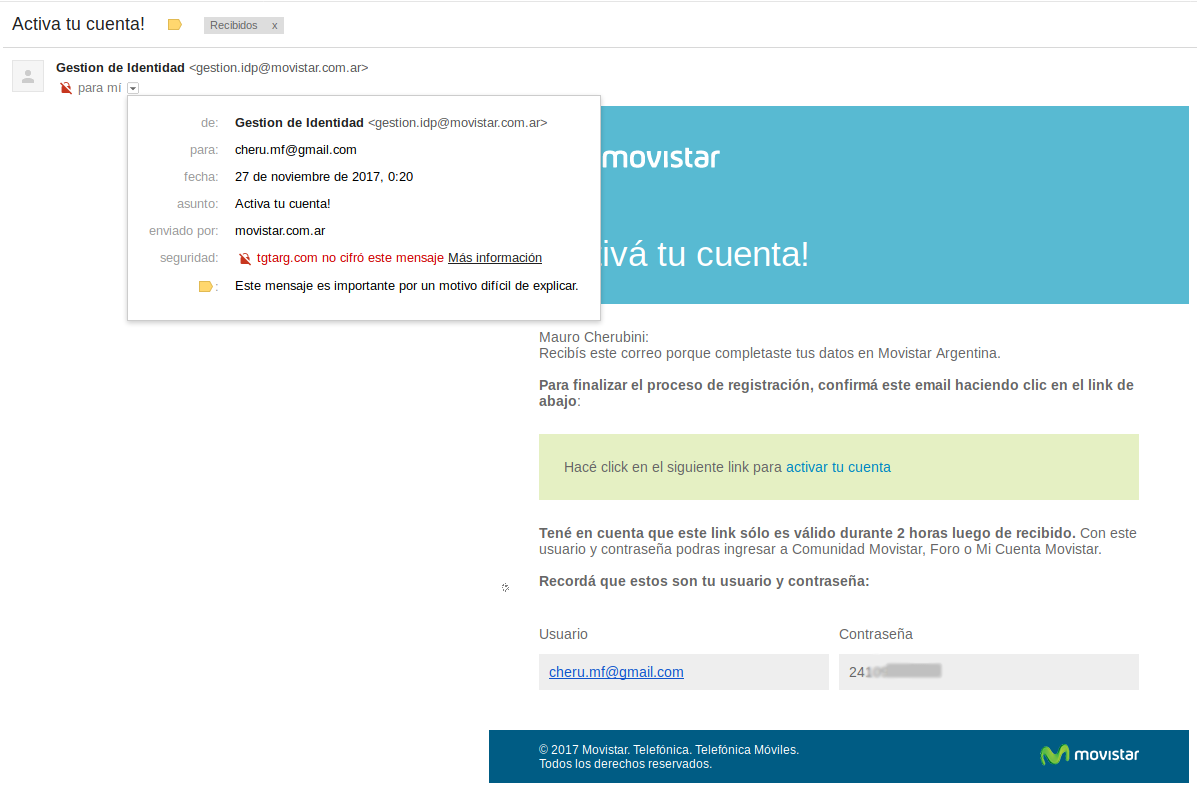
\includegraphics[scale=0.4]{images/mail_movistar_cheru_v3.png}}
\caption{Mail de validación de cuenta de mail de Movistar}
\end{figure}

\subsubsection{Diario La Nación}
Este es un sitio de masiva concurrencia, al solamente ingresar al sitio y analizar el tráfico que genera el mismo, observamos que se trata de un site de los denominados mixtos (si bien al ingresar uno en el browser observar que el link es https, muchos de los servicios que se consumen de forma interna son http).

\begin{figure}[H]
\centerline{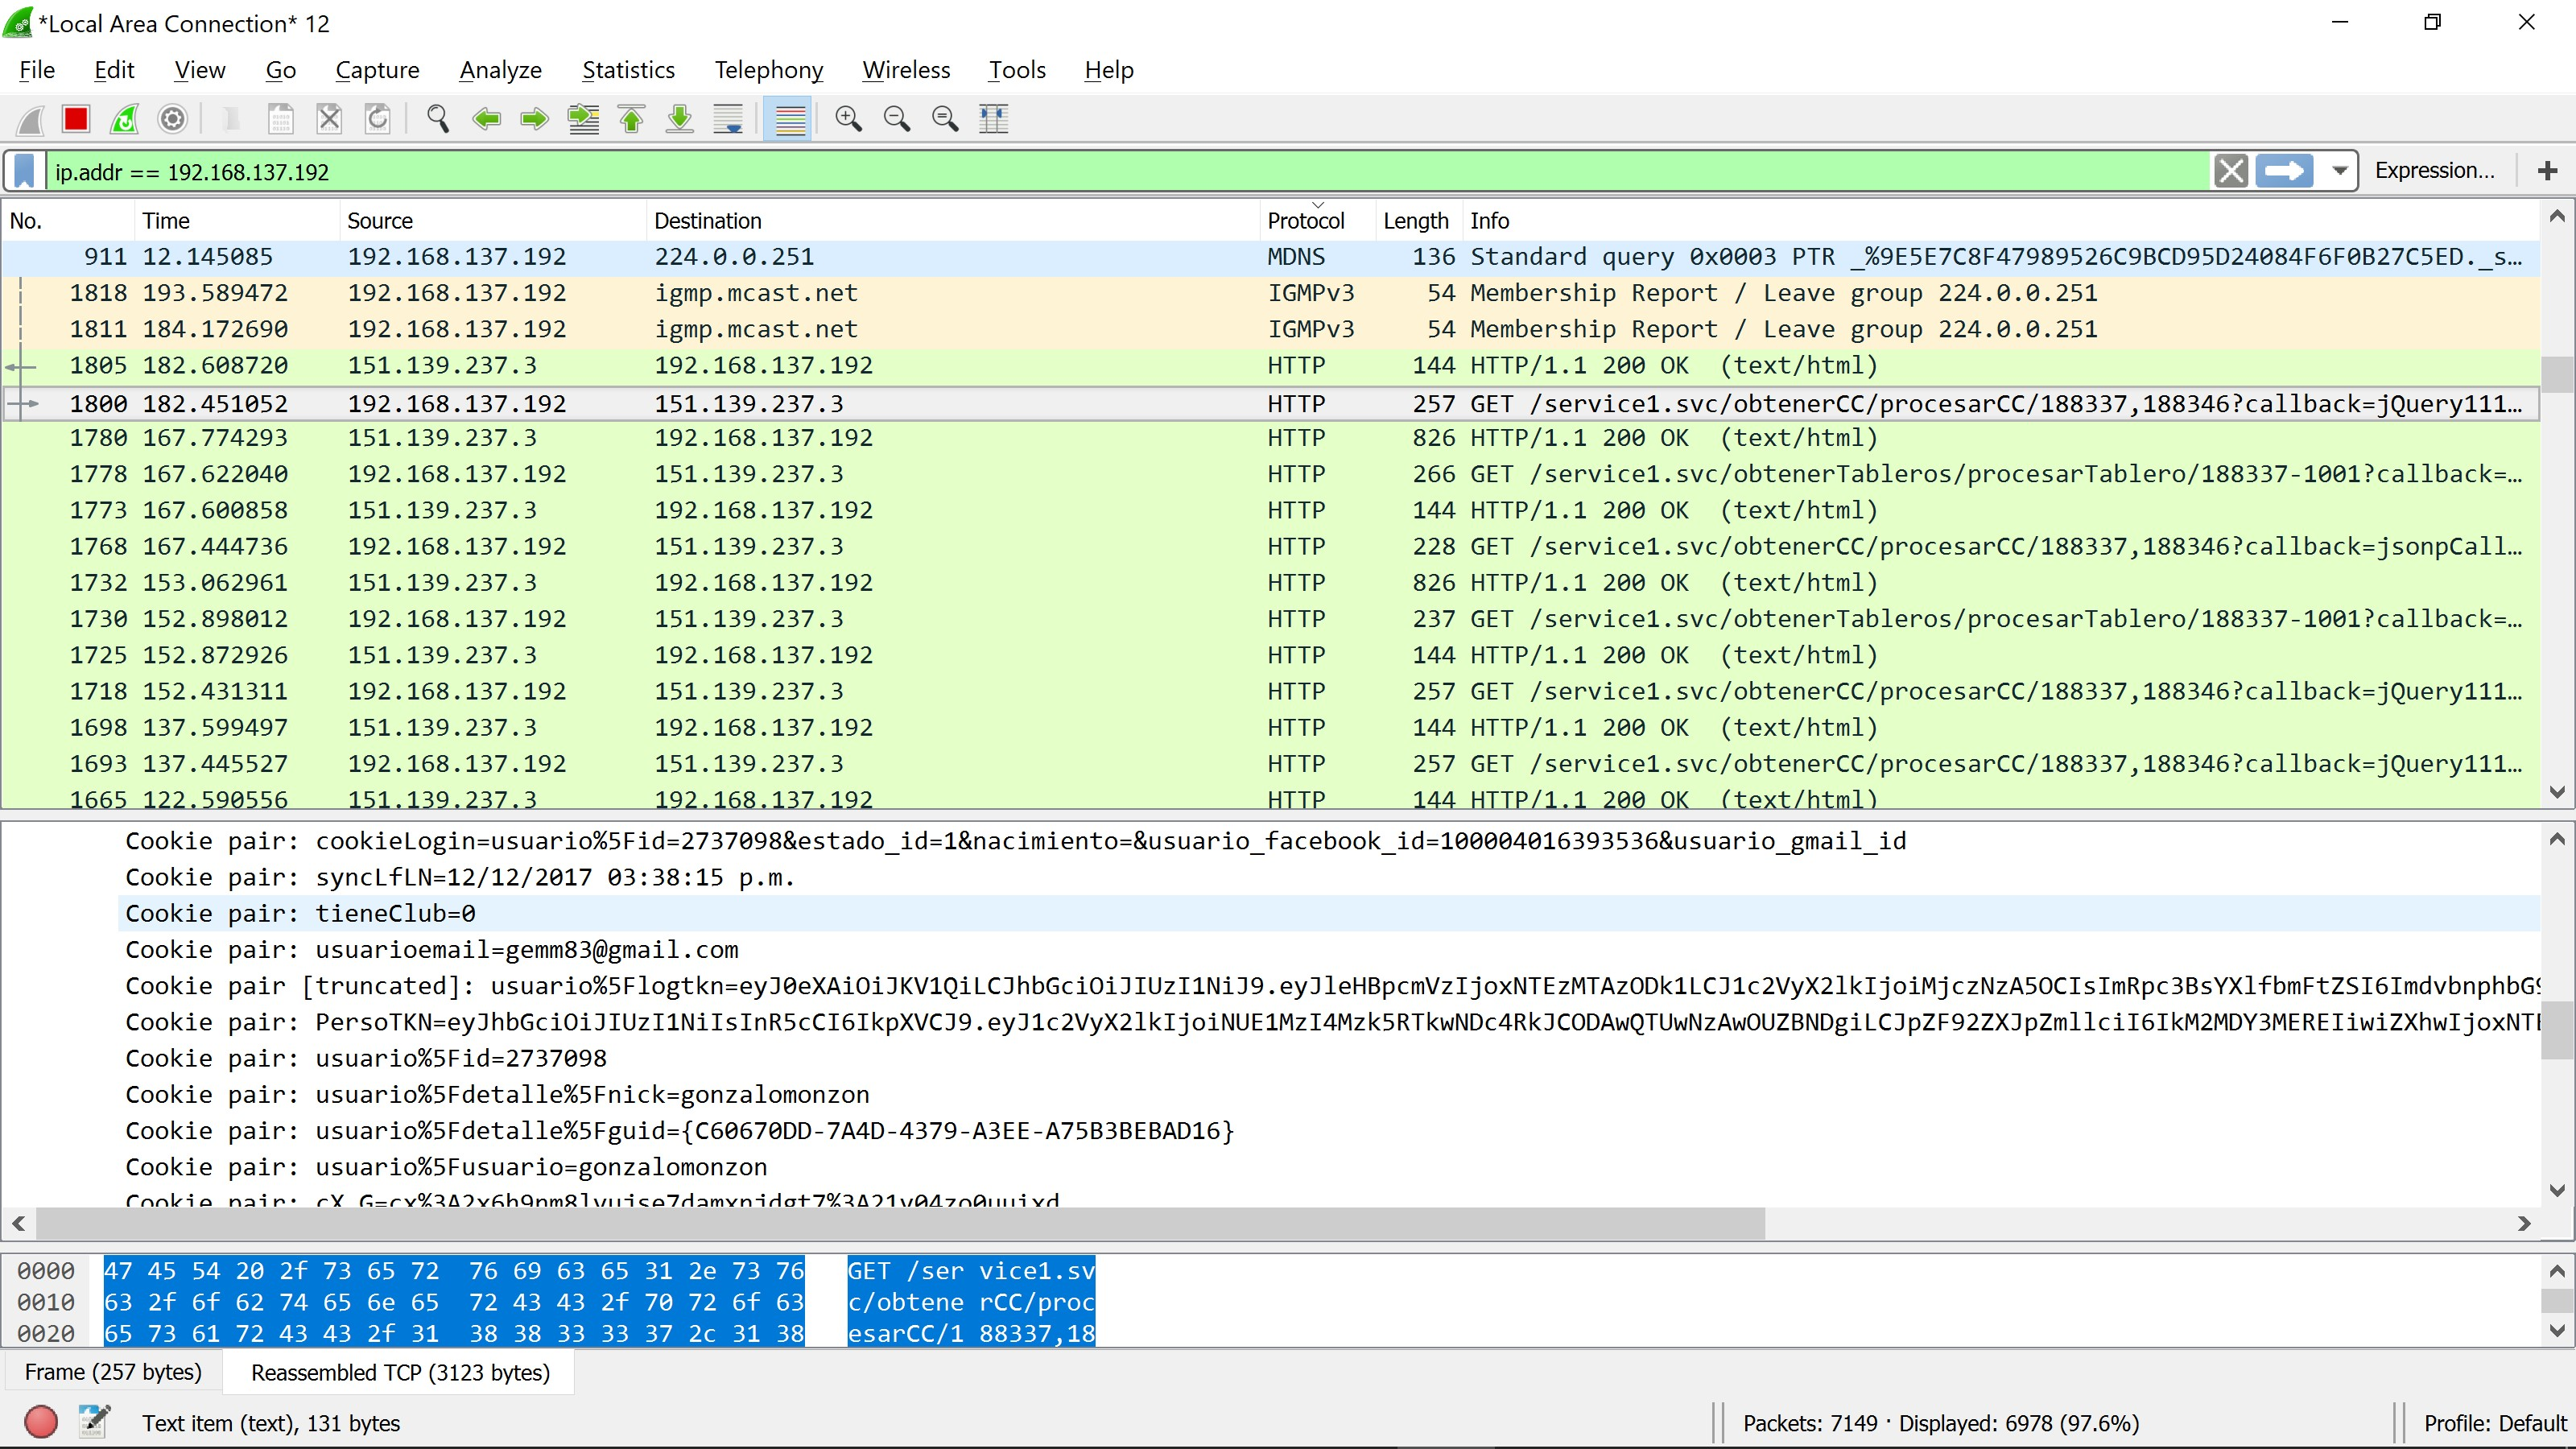
\includegraphics[scale=0.2]{images/lanacion.jpg}}
\caption{Trafico de La Nación}
\end{figure}

Podemos observar en la línea seleccionada con gris con una simple captura de Wireshark, como el contenido del paquete, tiene información importante, que podría potencialmente ser usada por atacantes (como el email, fecha de nacimiento, el id del usuario de Facebook con el que nos registramos, etc)

\pagebreak

\subsection{IOT}

\begin{figure}[H]
\centerline{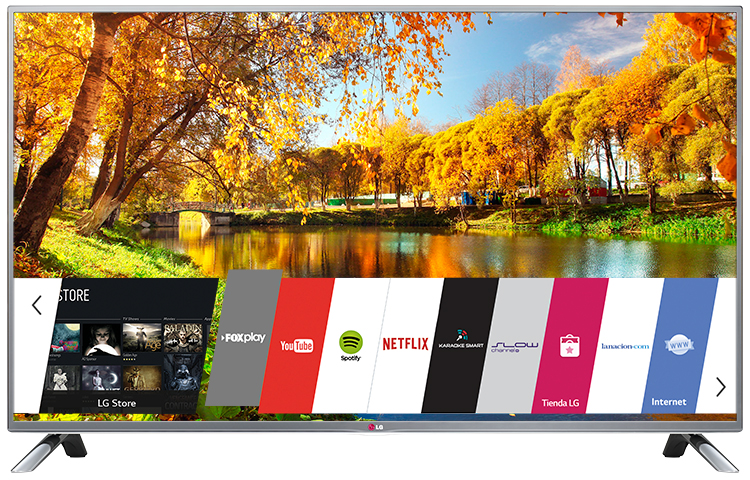
\includegraphics[scale=0.33]{images/LG_LB6500.jpg}}
\caption{}
\end{figure}

Con el objetivo de extender el análisis de dispositivos hogareños no solo a aquellos dispositivos móviles o a las típicas \textit{desktops} y \textit{notebooks}, decidimos analizar el tráfico generado por un \textit{Smart Tv} y su seguridad asociada. Entre otras aplicaciones decidimos analizar la seguridad usada en una aplicación tan común para estos dispositivos como lo es Netflix.
Para ello capturamos todos los paquetes enviados durante el uso de esta aplicación, y con dicha captura comprobamos que todo el tráfico asociado a ella viaja por medio de HTTP sin mayor seguridad. Examinando el contenido de los paquetes nos encontramos con solicitudes a distintos recursos, mayormente imágenes por ejemplo de las portadas de cada de serie que aparecen en el menú inicial, algunos otros en cambio parecían ser algún tipo de \textit{scripts}. Si bien no se hizo un análisis profundo de manera de identificar su uso y funcionamiento este tipo de falencias de seguridad podría llegar a resultar en algún \textit{exploit}. 


%Dado que hoy en día, la mayoría de los artefactos tienen conexión a internet, nos propusimos revisar un poco un Smart TV en cual conectamos a la red wifi.

%Como primera opción usamos la app de Netflix que viene instalada en el so del equipo, y encontramos que la misma funcionaba según lo esperado, es decir, todo el tráfico iba por un canal seguro sobre TCP, sin enviar paquetes sobre protocolos no cifrados.

%Pasamos el Smart a modo televisor (sin hacer nada con la red supuestamente) y observamos que en modo televisor y todo (sin usar ningún tipo de software más que el sistema operativo) se enviaron un montón de paquetes de forma insegura (dado que el único soft actualmente corriendo era el so, se lo adjudicamos a búsqueda de actualizaciones de software, envío de datos estadísticos, etc) lo mismo pasaba con el Smart en modo StandBy, es decir, estando conectado a la red, un Smart continuamente está enviando información en paquetes inseguros (al menos este modelo de LG, pero estimamos que la mayoría se comportan de formas similares) que podría llegar a ser utilizada por cualquier atacante.
    
\begin{figure}[H]
\centerline{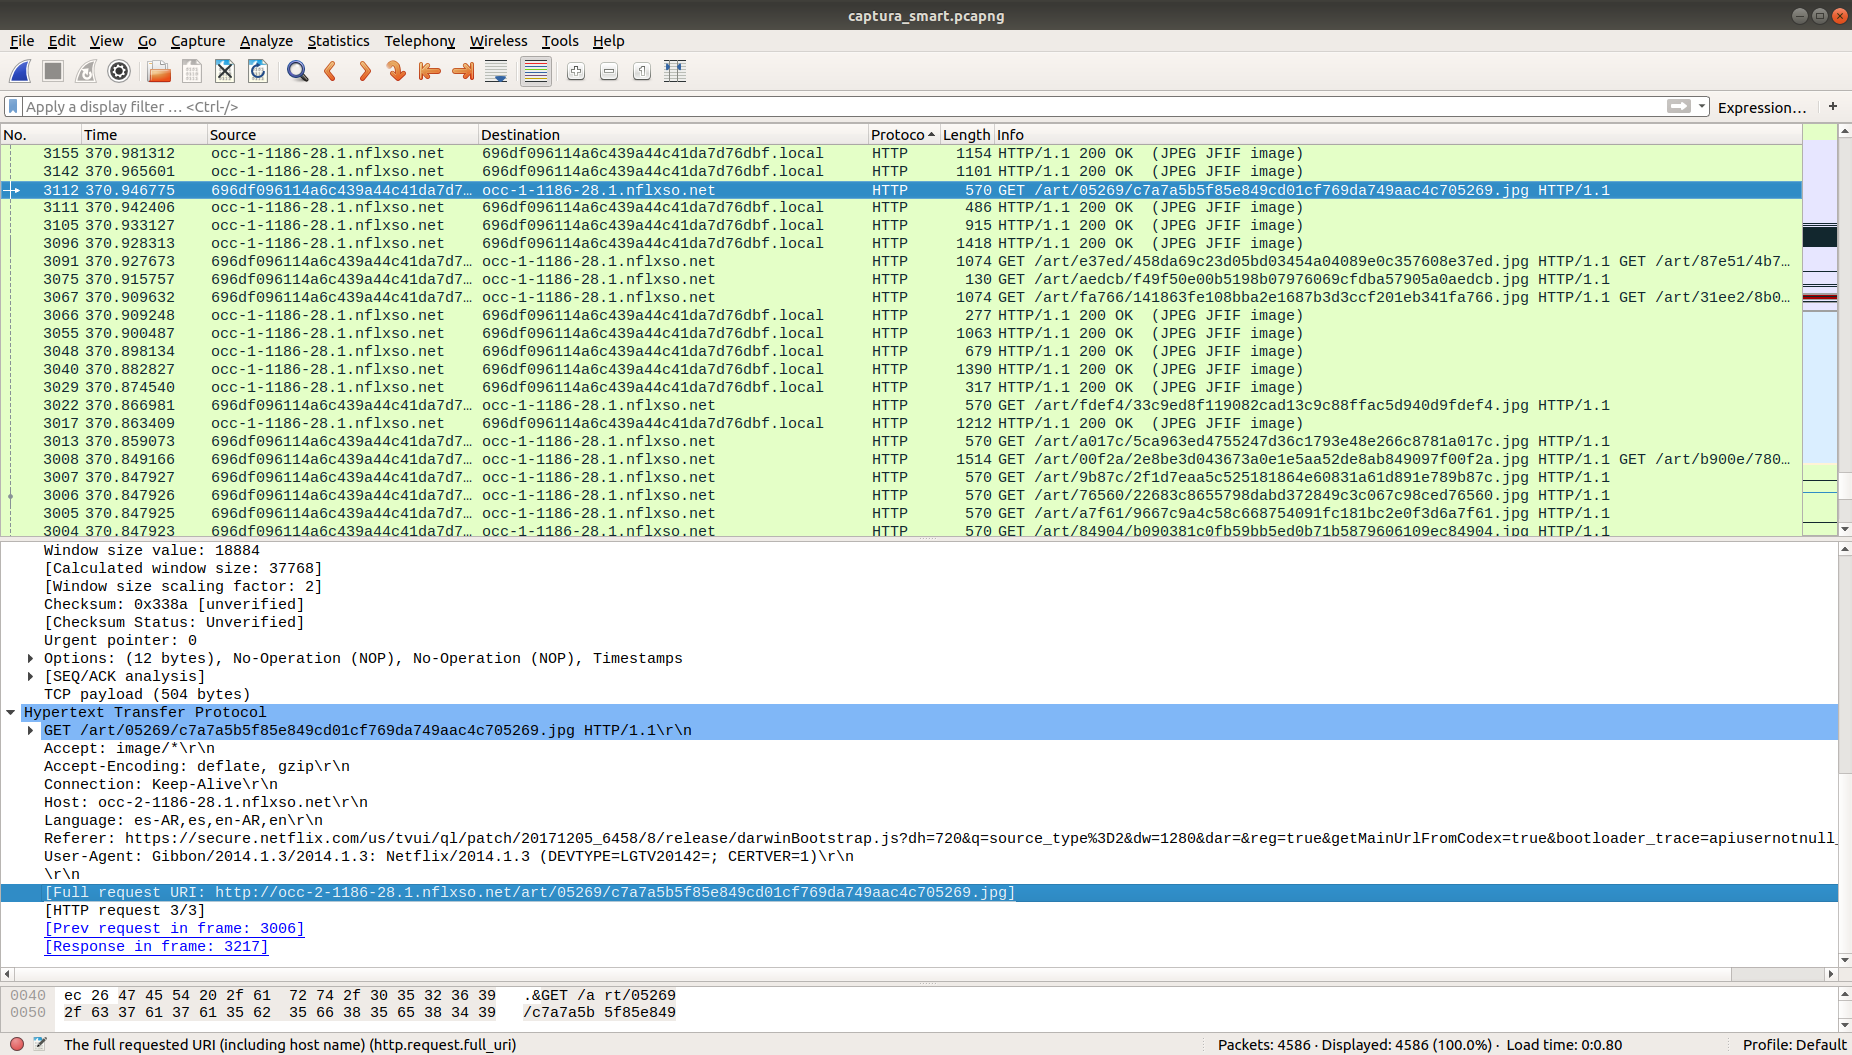
\includegraphics[scale=0.33]{images/captura_smart_tv.png}}
\caption{}
\end{figure}

\subsection{Ataques}

Continuamos analizando la seguridad de algunos sitios web en base al uso de las técnicas y herramientas investigadas. Para ello utilizamos la técnica de SSLSplit mediante la herramienta de \textit{Burp Suite}, que funciona como un \textit{proxy} y permite mediante un simple botón de \textit{CA Certificate} descargar un certificado apócrifo del sitio que intentamos vulnerar.
%En base a las herramientas y técnicas investigadas continuamos analizando la seguridad de algunos sitios web con el objetivo de obtener datos

%Analizamos la seguridad de algunos sitios en busca de corroborar el nivel de seguridad que poseen, para esto utilizamos la herramienta de \textit{Burp Suite} que funciona como un proxy, y nos brinda un certificado (originalmente cuando se arranca la herramienta, el certificado para instalar se puede descargar desde http://burp)

\begin{figure}[H]
\centerline{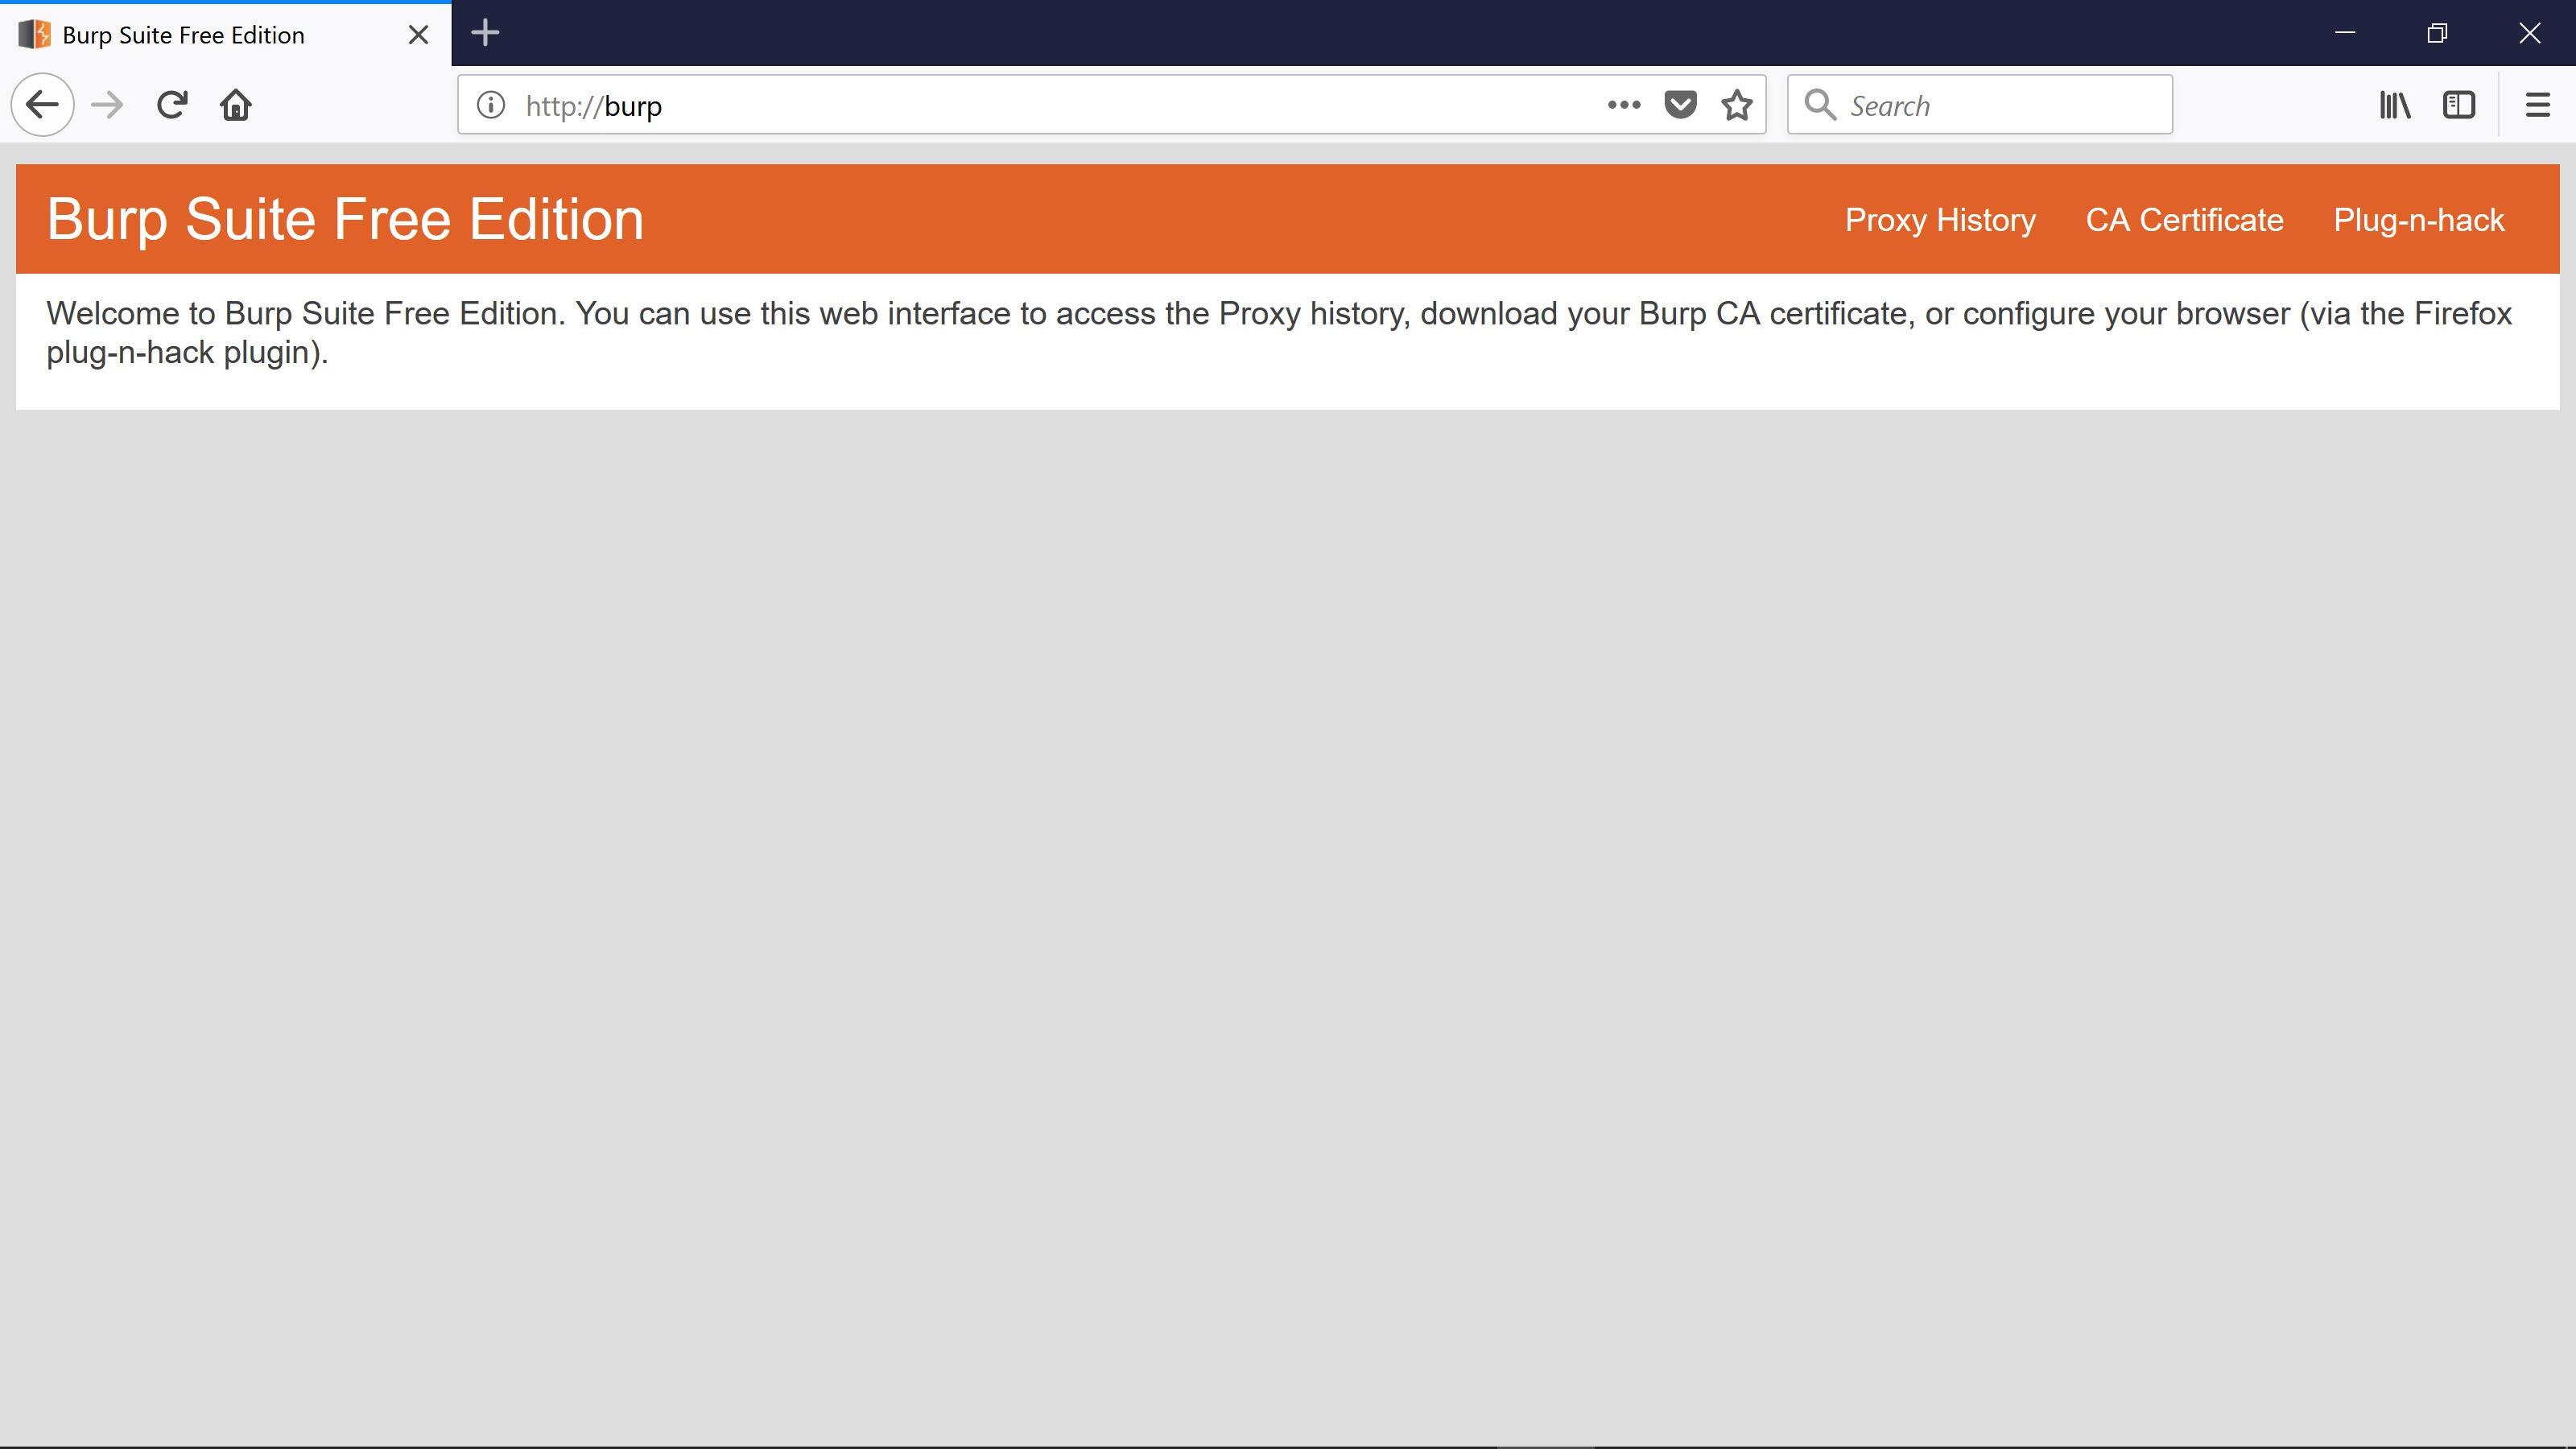
\includegraphics[scale=0.4]{images/certificado.jpg}}
\caption{}
\end{figure}

%Presionando el botón denominado CA Certicate descargamos el certificado y lo instalamos en la máquina, de esta forma ahora el certificado de la herramienta es un certificado confiable y lo podemos usar sin inconvenientes.

%Otra forma de usarlo un poco más laboriosa, es con un browser navegar al sitio que queramos, este nos va a avisar que el certificado no es confiable, pero podemos elegir continuar. De esta forma no hace falta instalar el certificado, aunque el trabajo se vuelve más tedioso dado que tenemos que realizar esta misma operación por cada sitio que queramos visitar.

%Los paquetes puestos en el informe son recortados para poder observar solo la parte importante.

\subsubsection{Sitio Santander Río}

Con el objetivo de intentar comprobar la seguridad del sistema de \textit{login} dentro del \textit{homebanking} del sitio, intentando capturar paquetes que contengan datos sensibles como el nombre usuario, número de cuenta, contraseña, etc. Al analizar el contenido de estos paquetes tras instalar el certificado, observamos que el sitio encripta los datos sensibles por software, de manera que es mucho más difícil realizar un ataque sobre este sitio, lo cual es esperable de un sitio de \textit{homebanking} en donde la confidencialidad de estos datos debería ser prioritario.

Observamos el contenido del paquete de POST (que viaja por HTTPS) asociado al \textit{login}:
\newline
\newline
dniOri=30654408\&dni=330A330A330A102A330A282A297A239A239A330A57A\newline\&clave=330A330A330A330A330A271A349A102A\newline\&claveNueva=\newline\&claveNuevaReingreso=\newline\&usuario=228A250A30A77A340A16A282A250A315A315A315A315A315A315A315A315A315A315A315A315A\newline\&usuarioNuevo=\newline\&fechaNac=\newline\&usuarioVacio=315A315A315A315A315A315A315A315A315A315A315A315A315A315A315A315A31\newline\&claveVacia=330A330A330A330A330A330A330A330A
\newline

Como detalle observamos que el DNI viaja en claro, no sería de tanta prioridad en el sentido de que no es un dato difícil de conseguir por medio de otros servicios si uno conoce algún otro dato básico como el nombre y apellido, pero podría ser utilizado para derivar otros datos o conocer la identidad de ciertas personas en caso de que se trate de una conexión en algún lugar como un hogar de familia.

\subsubsection{Sitio Hotmail}
En este sitio obtuvimos resultados diferentes a los esperados, en base a la instalación de un certificado falso pudimos obtener en claro el nombre de usuario y la contraseña con la cual los usuarios de nuestra red accedieron a su correo electrónico.

Observamos el contenido del paquete de POST (que viaja por HTTPS) asociado al \textit{login}:
\newline
\newline
\&login=gemm83@hotmail.com\newline\&loginfmt=gemm8@hotmail.com\newline\&type=11\newline\&LoginOptions=3\newline\&lrt=\newline\&lrtPartition=\newline\&hisRegion=\newline\&hisScaleUnit=\newline\&passwd=AllYouNeedIsThink\newline\&ps=2\newline\&psRNGCDefaultType=
\newline\newline
Como observamos los valores de los campos de \textit{login} y \textit{passwd} que tienen el nombre de usuario y la contraseña respectivamente, ambos sin encriptar con lo cual el atacante podrá en base a estos datos adueñarse de la cuenta.
A diferencia de este en otros sitios como \textit{Gmail} el envío de estos datos se realiza por el contrario mediante otra encriptación extra de capa de aplicación, por lo que a los atacantes que apelen a esta técnica no les alcanzará para adueñarse de la cuenta.

%ingresando a su cuenta, de esta forma con la simple aceptación de un certificado apócrifo, podemos robar información sensible.

%\subsubsection{Sitio Gmail}
%Acá observamos que el sitio envía los datos de manera encriptada al contrario del sitio de Hotmail, de esta forma con solo el certificado no alcance para obtener las credenciales.

\subsubsection{Sitio Bing}

\textit{Burp Suite} nos permitió poner en práctica un ataque de \textit{URL Spoofing} en la página de búsqueda de \textit{Bing}. Esto consiste en modificar las URL de la página interceptada, para lo cual seleccionamos "Match and Replace" y seleccionamos por medio de un patrón el segmento de la URL que queremos modificar.
%Para analizar este sitio usamos Burp para realizar un ataque de url spoofing (cambiar una url sin que el usuario se dé cuenta).
%Para esto vamos a utilizar una opción "Match and Replace" que nos permite indicándole cierta parte del mensaje http (header, body, etc) que busque un determinado patrón y lo reemplace por otro.

\begin{figure}[H]
\centerline{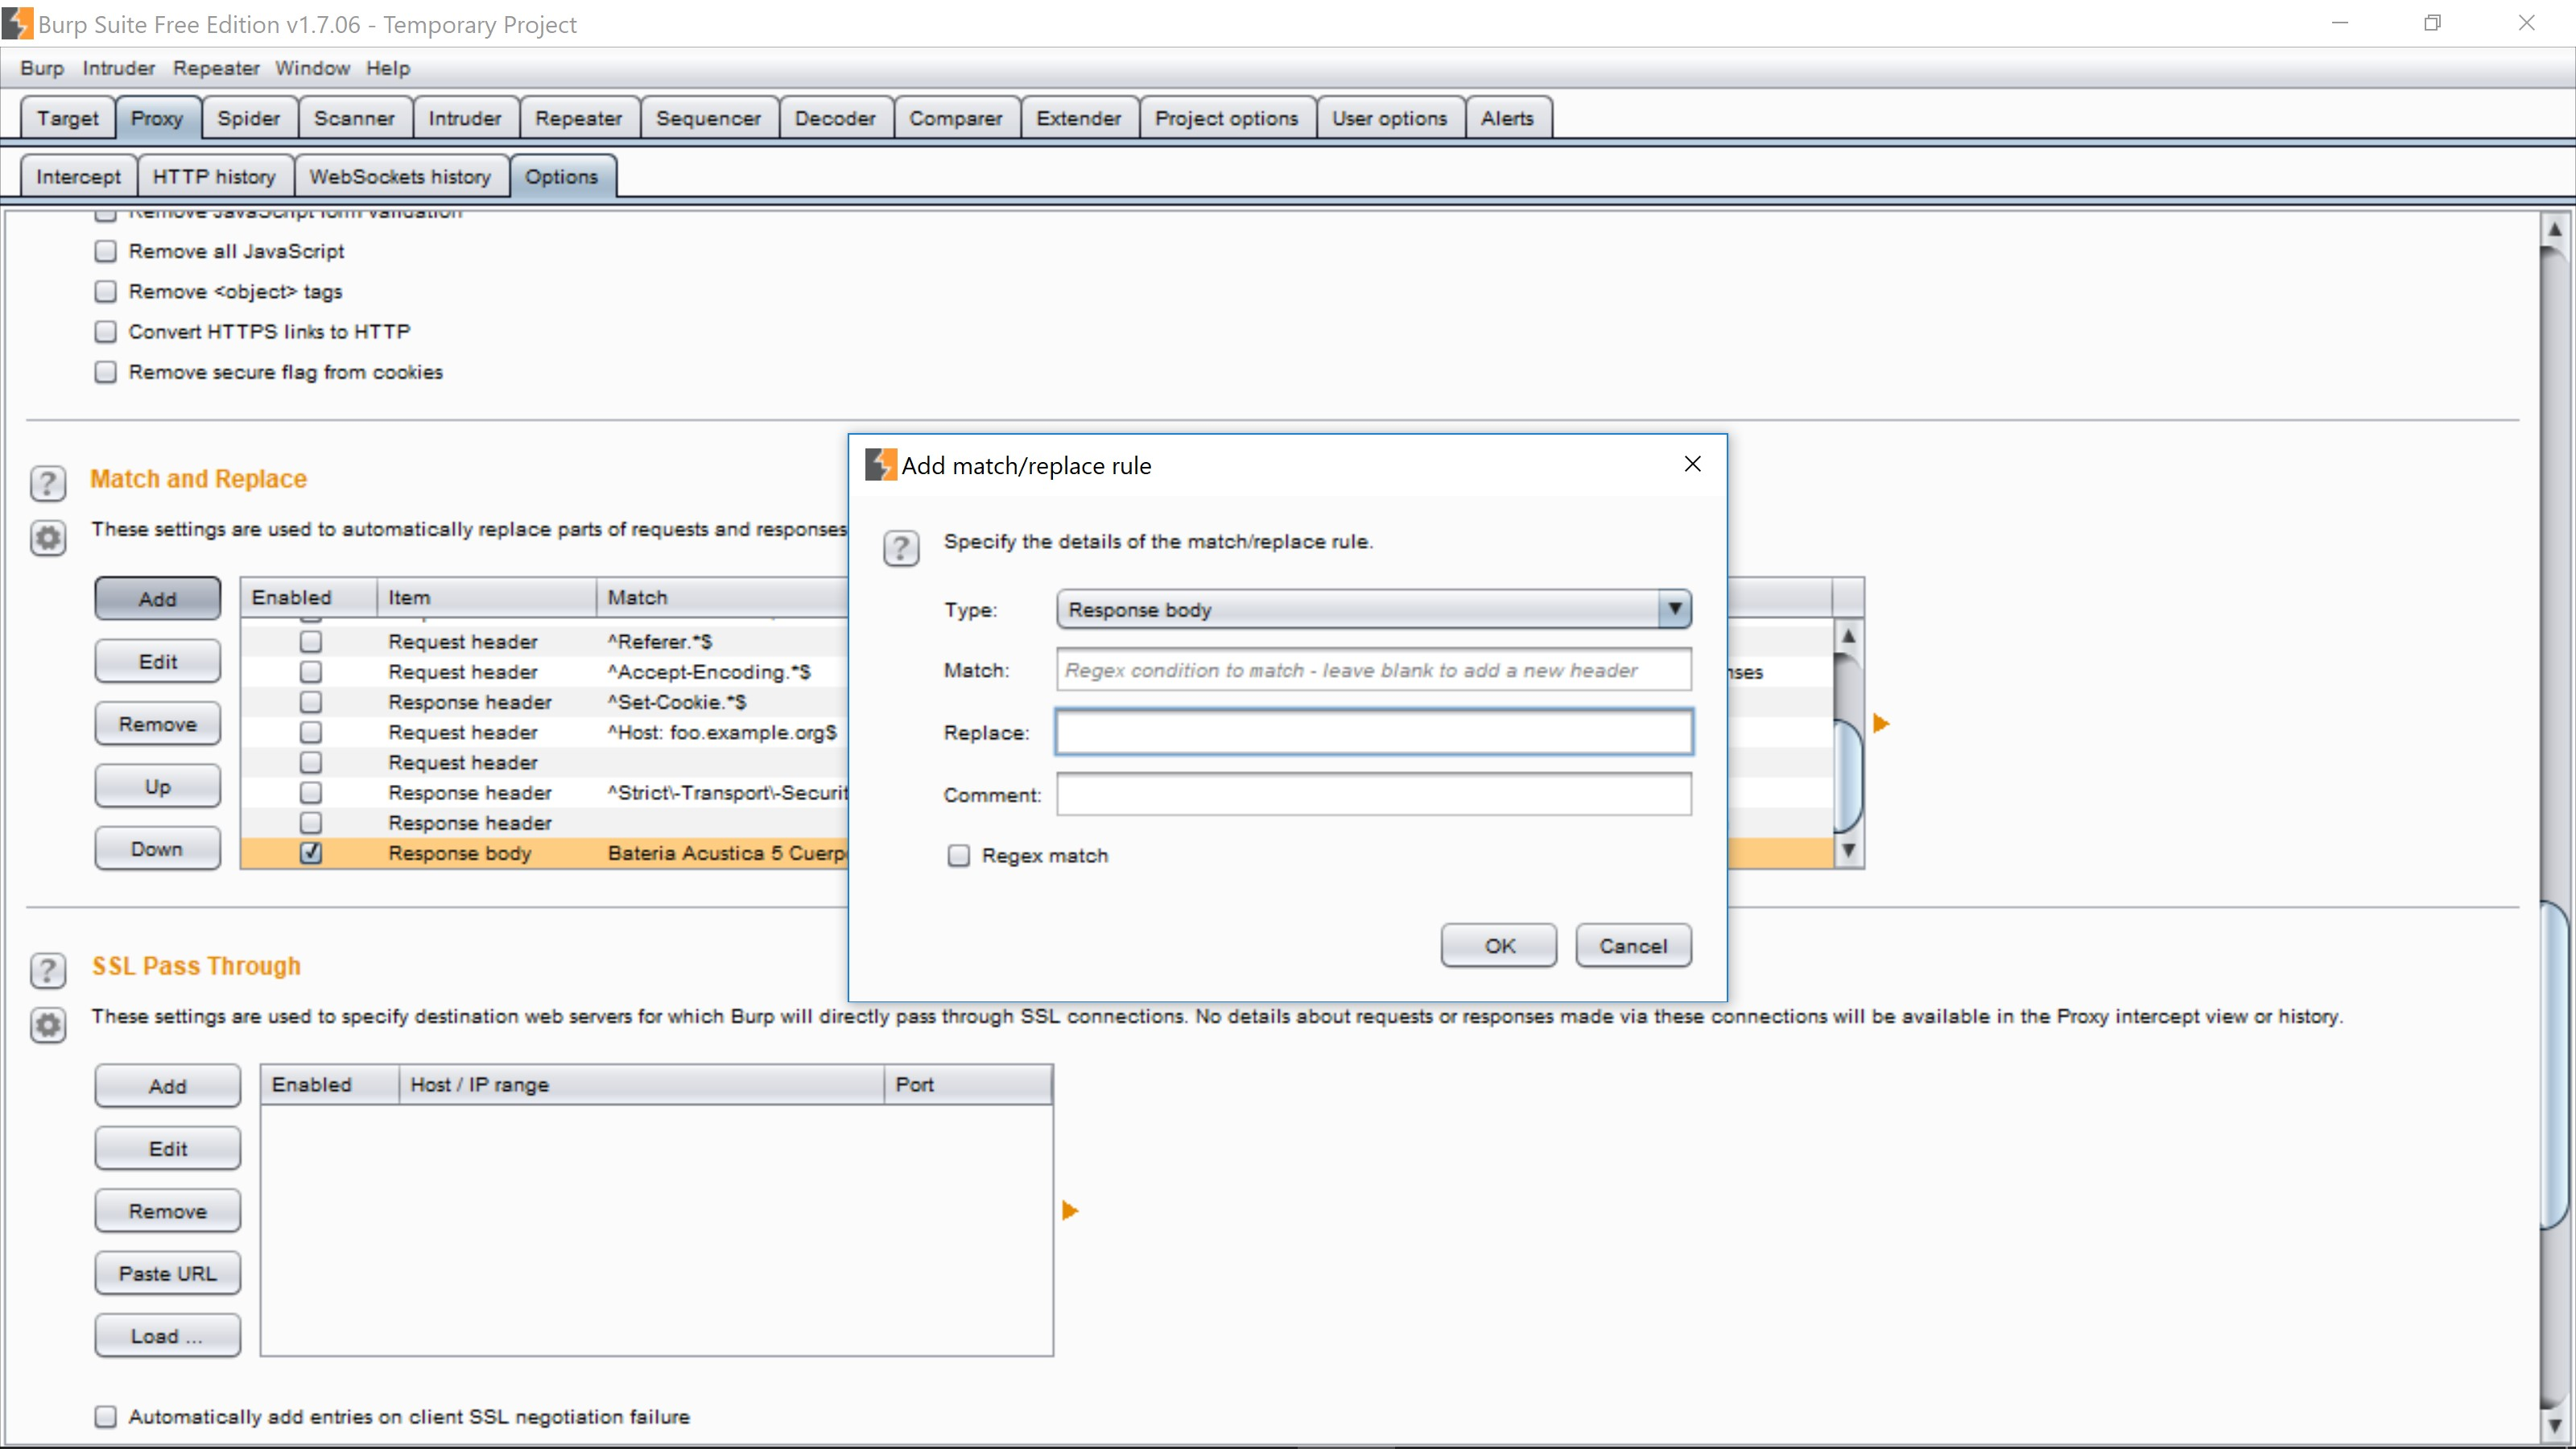
\includegraphics[scale=0.15]{images/match_and_replace.jpg}}
\caption{}
\end{figure}

Para hacer esta prueba, utilizamos una imagen de Google a modo de ejemplo, y reemplazamos la URL del recurso correspondiente a la imagen de fondo del sitio por la que conseguimos\newline

Antes\newline
\begin{figure}[H]
\centerline{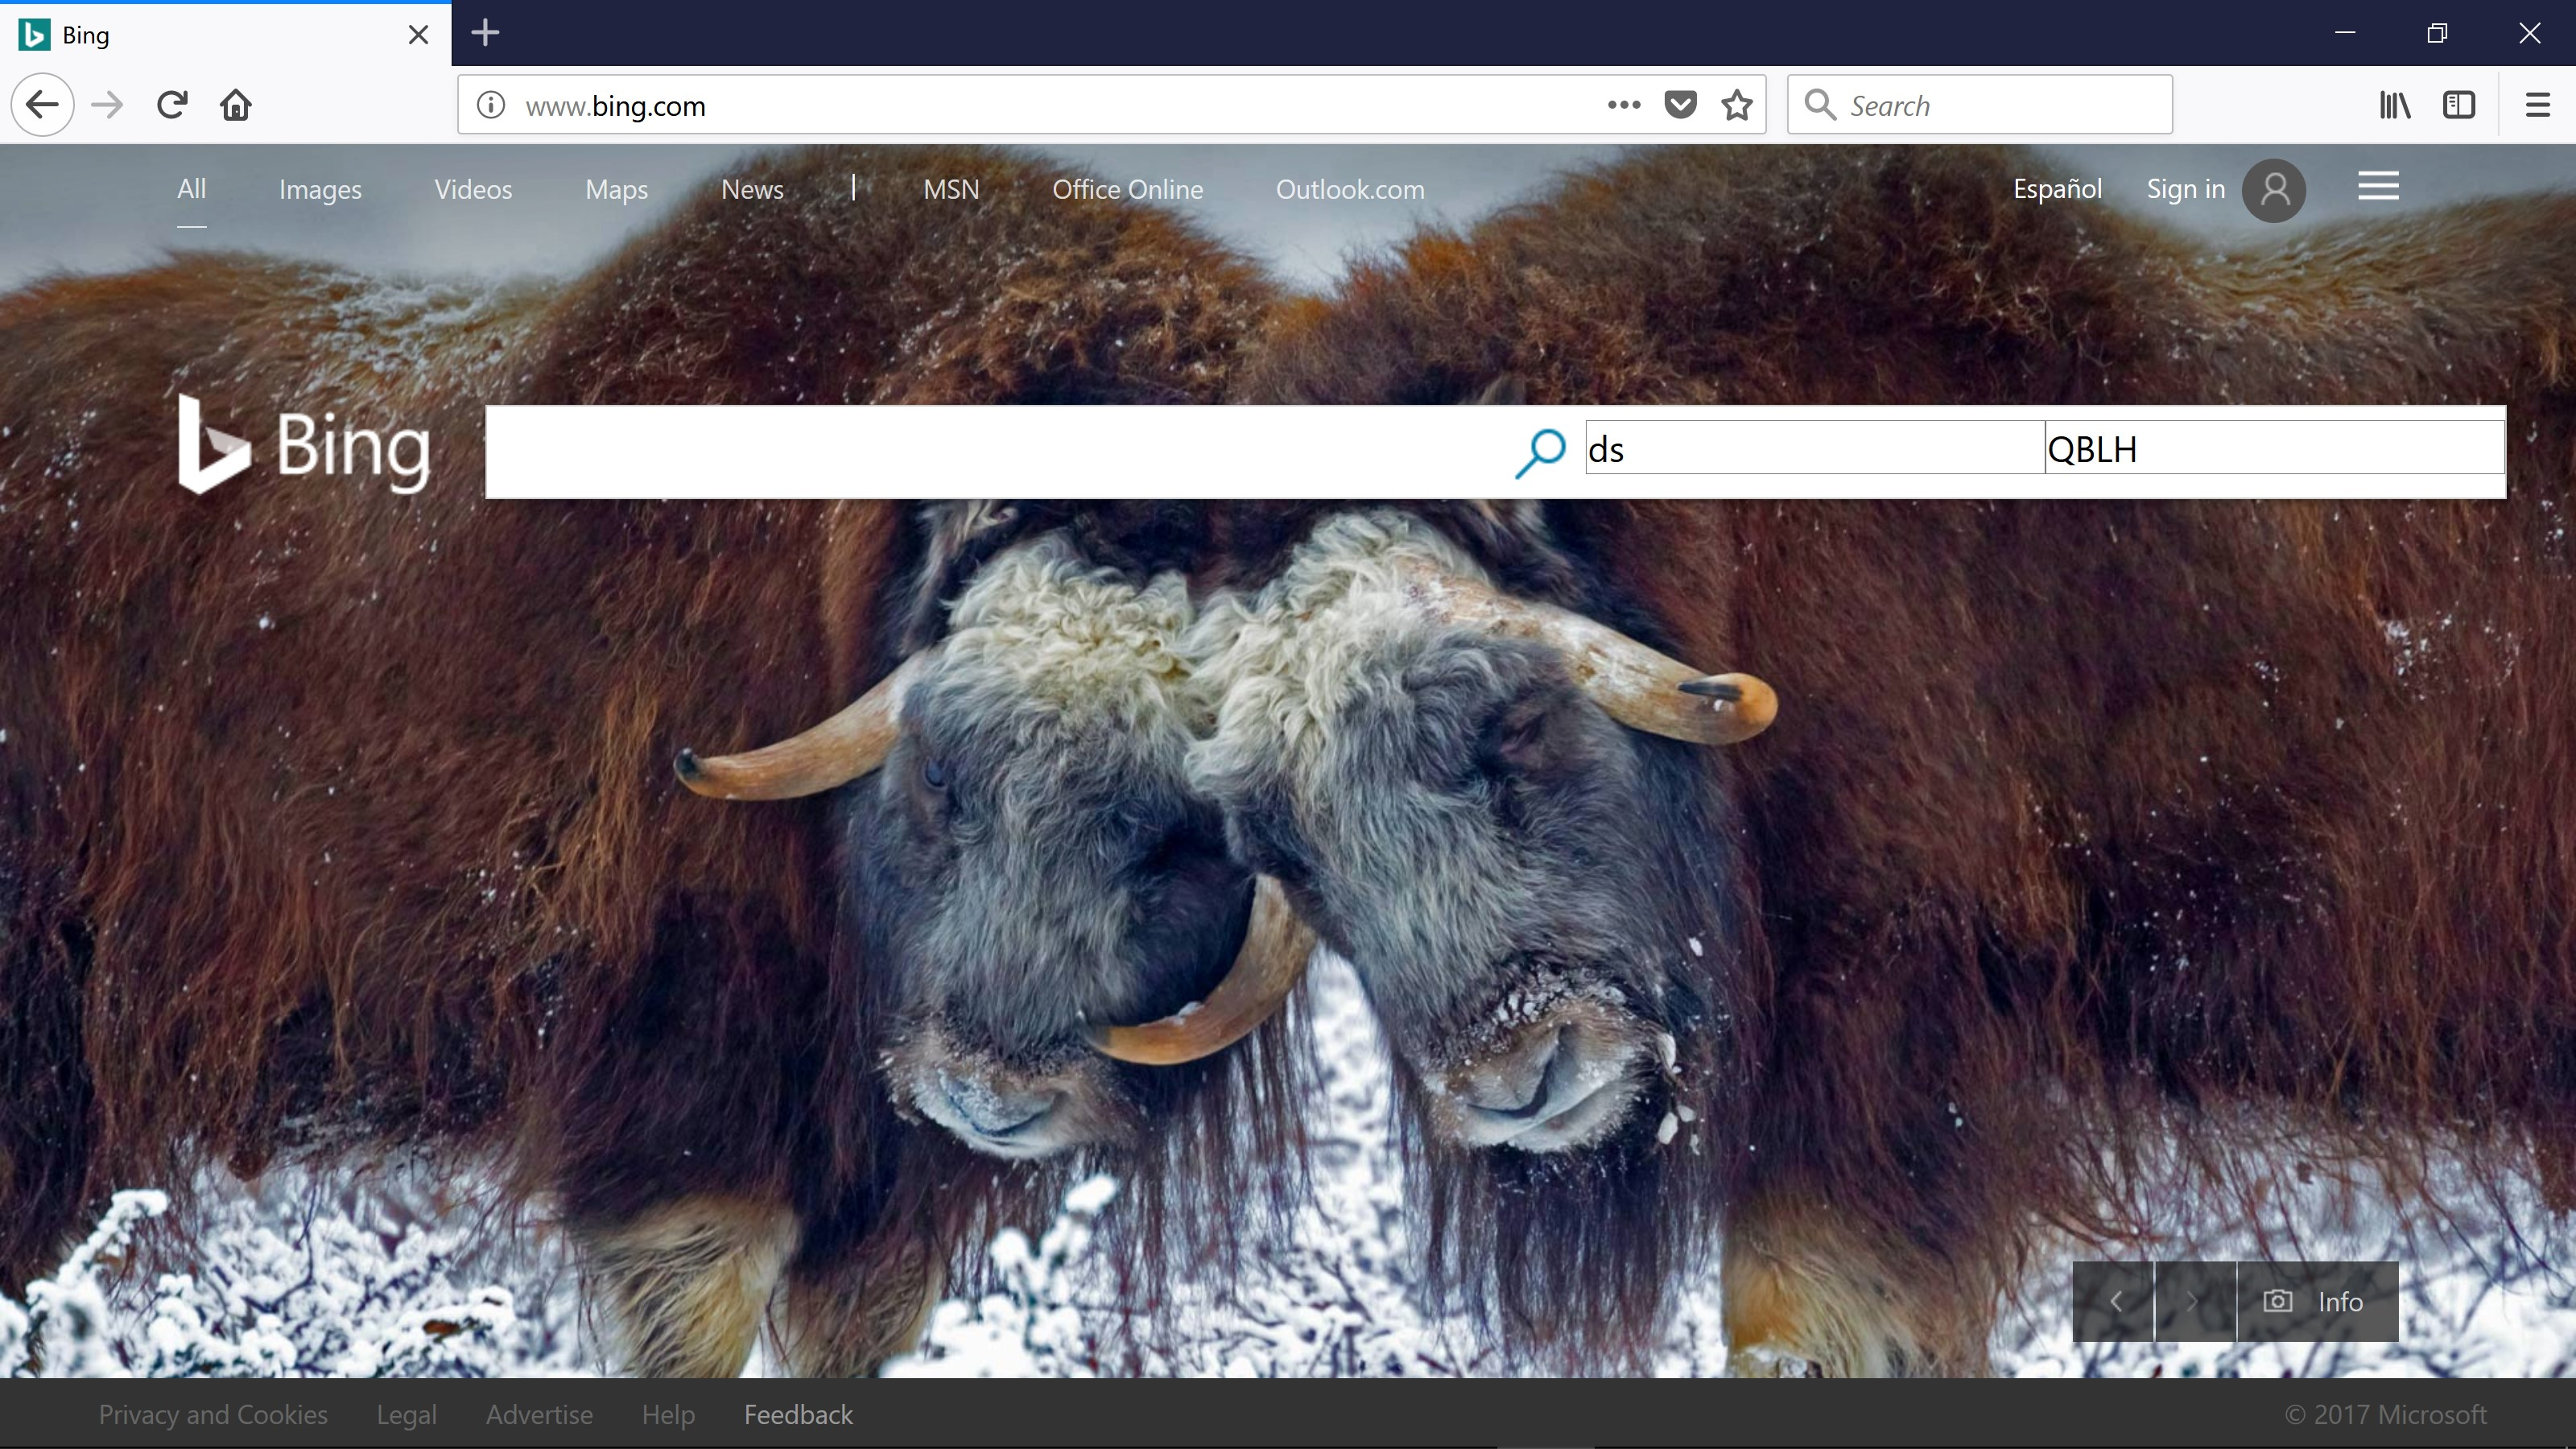
\includegraphics[scale=0.17]{images/bing_1.jpg}}
\caption{Pagina original}
\end{figure}
Después\newline
\begin{figure}[H]
\centerline{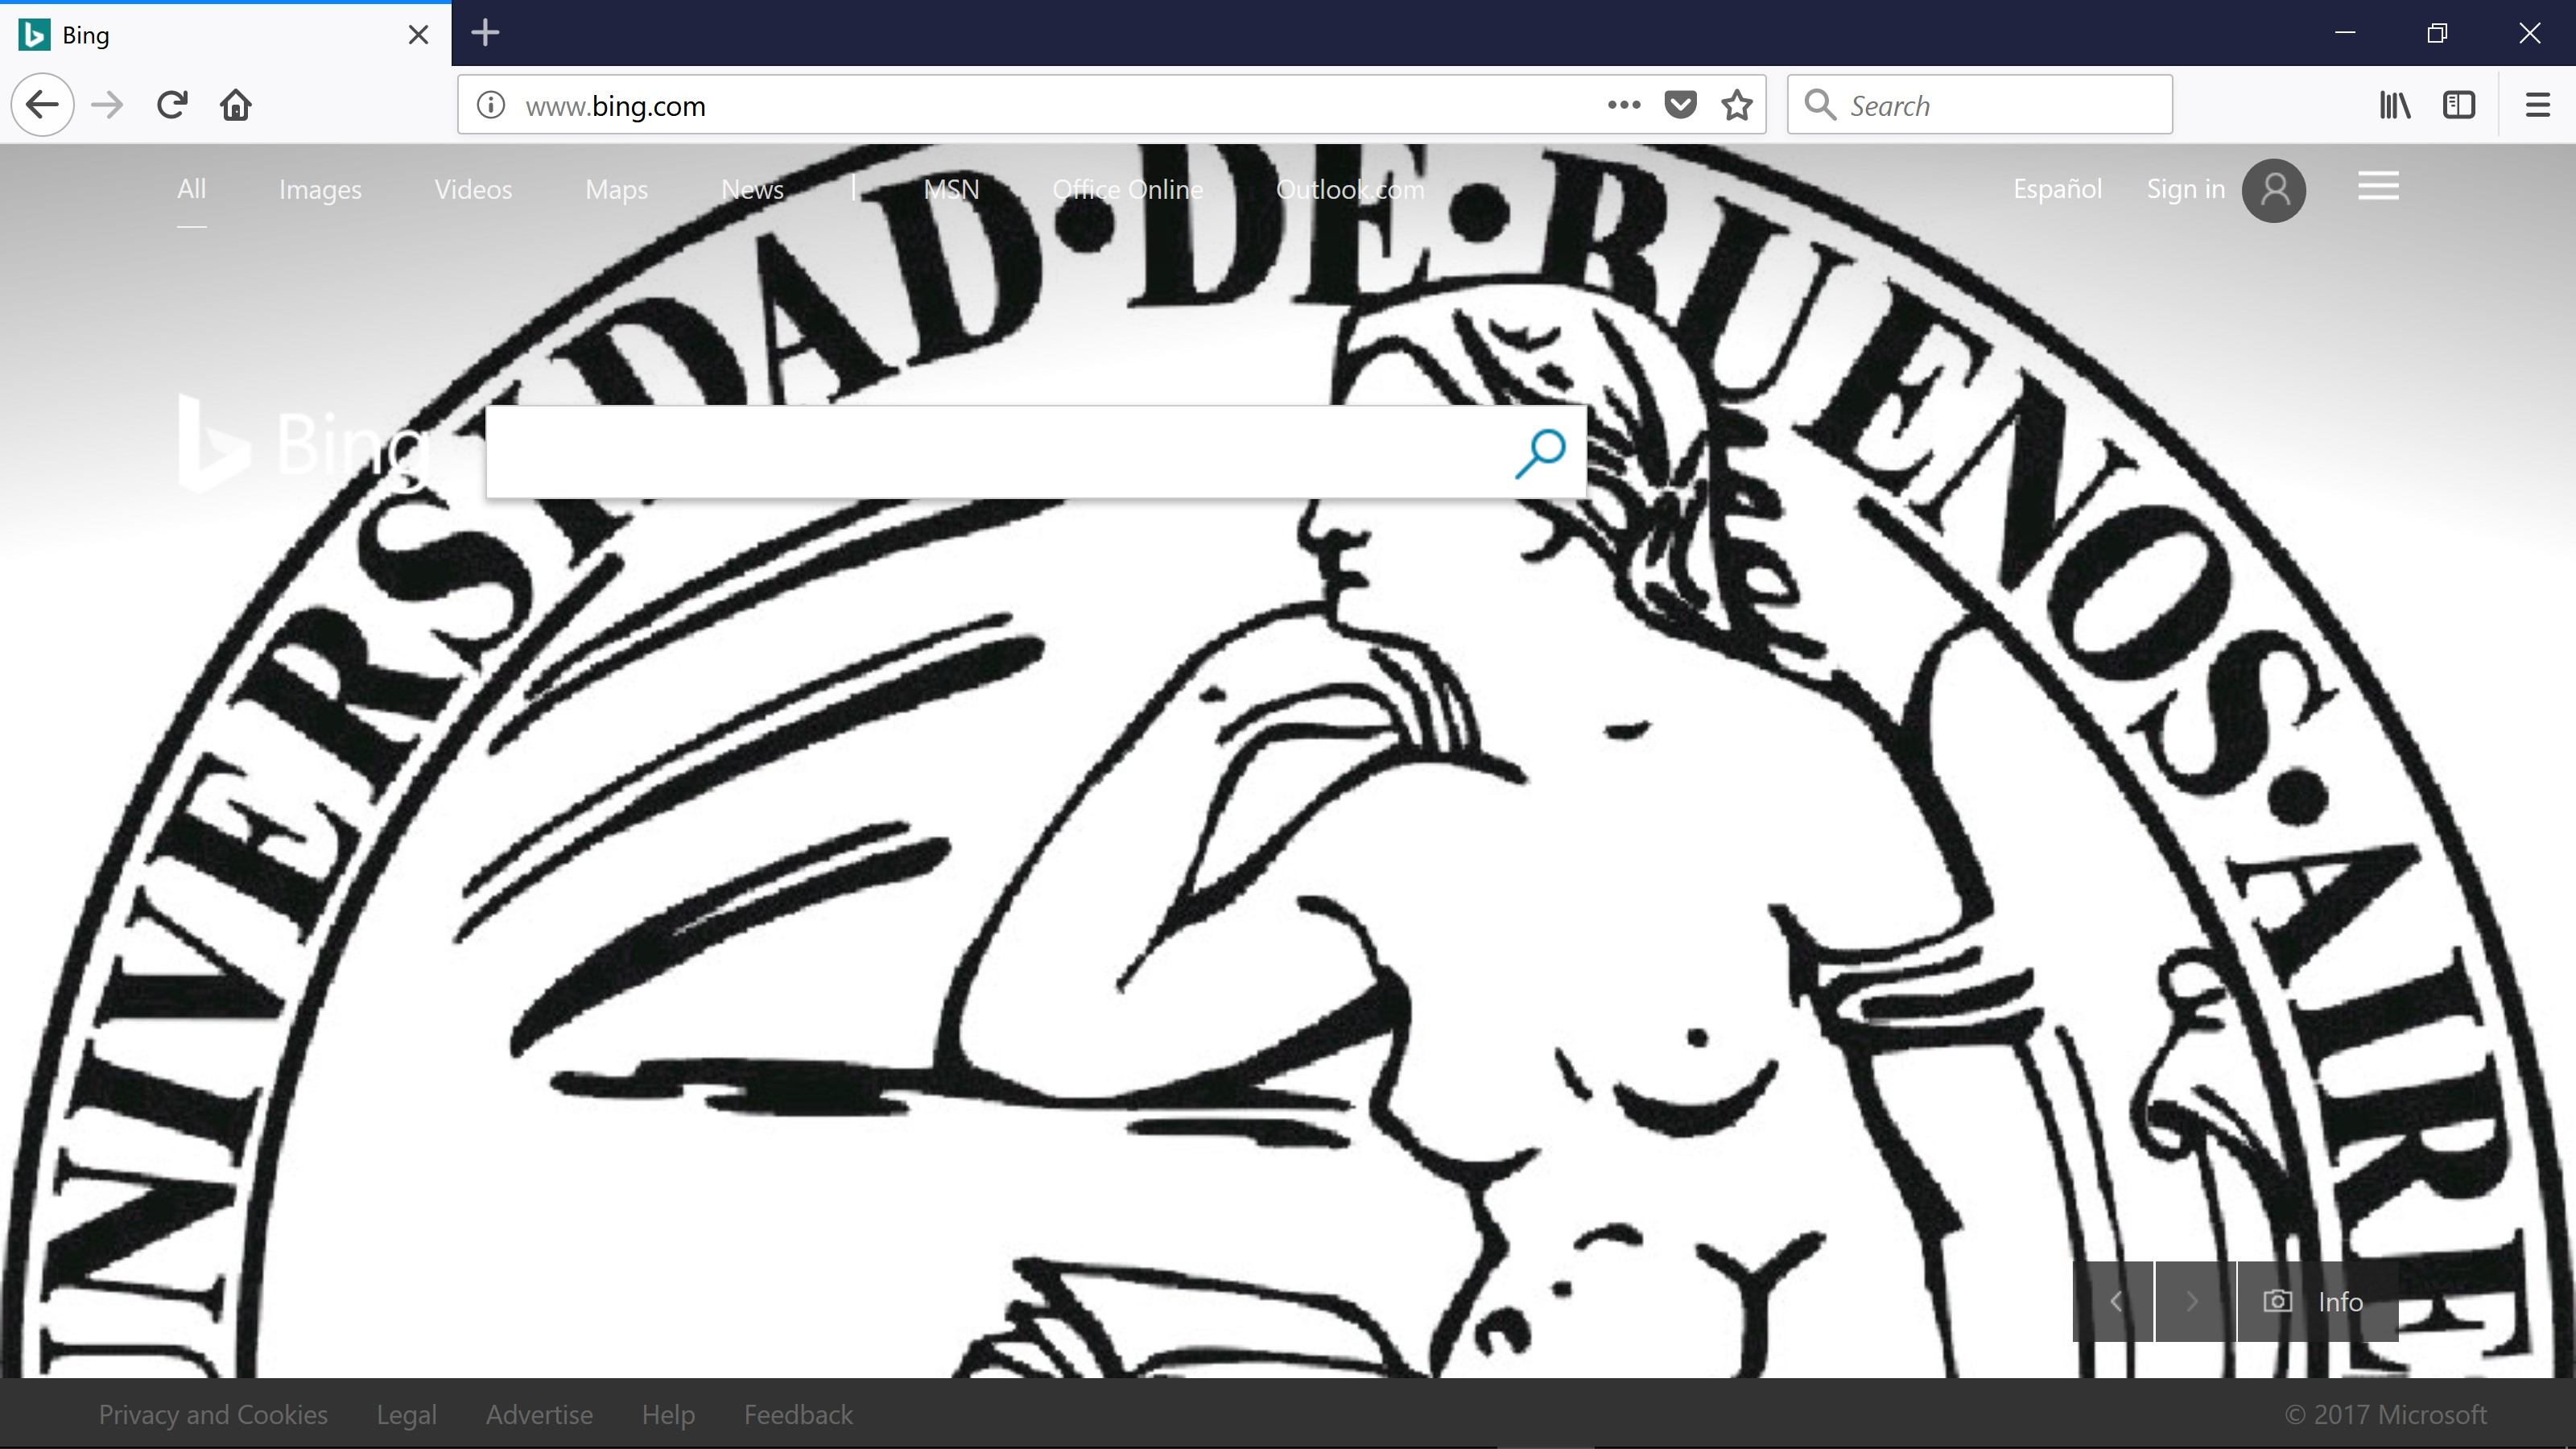
\includegraphics[scale=0.17]{images/bing_3.jpg}}
\caption{Pagina tras ser atacada por URL Spoofing}
\end{figure}

\subsubsection{Sitio MercadoLibre}
Realizamos el mismo ataque solo que en este caso reemplazamos texto y observamos el mismo resultado que antes.
\newline
\begin{figure}[H]
\centerline{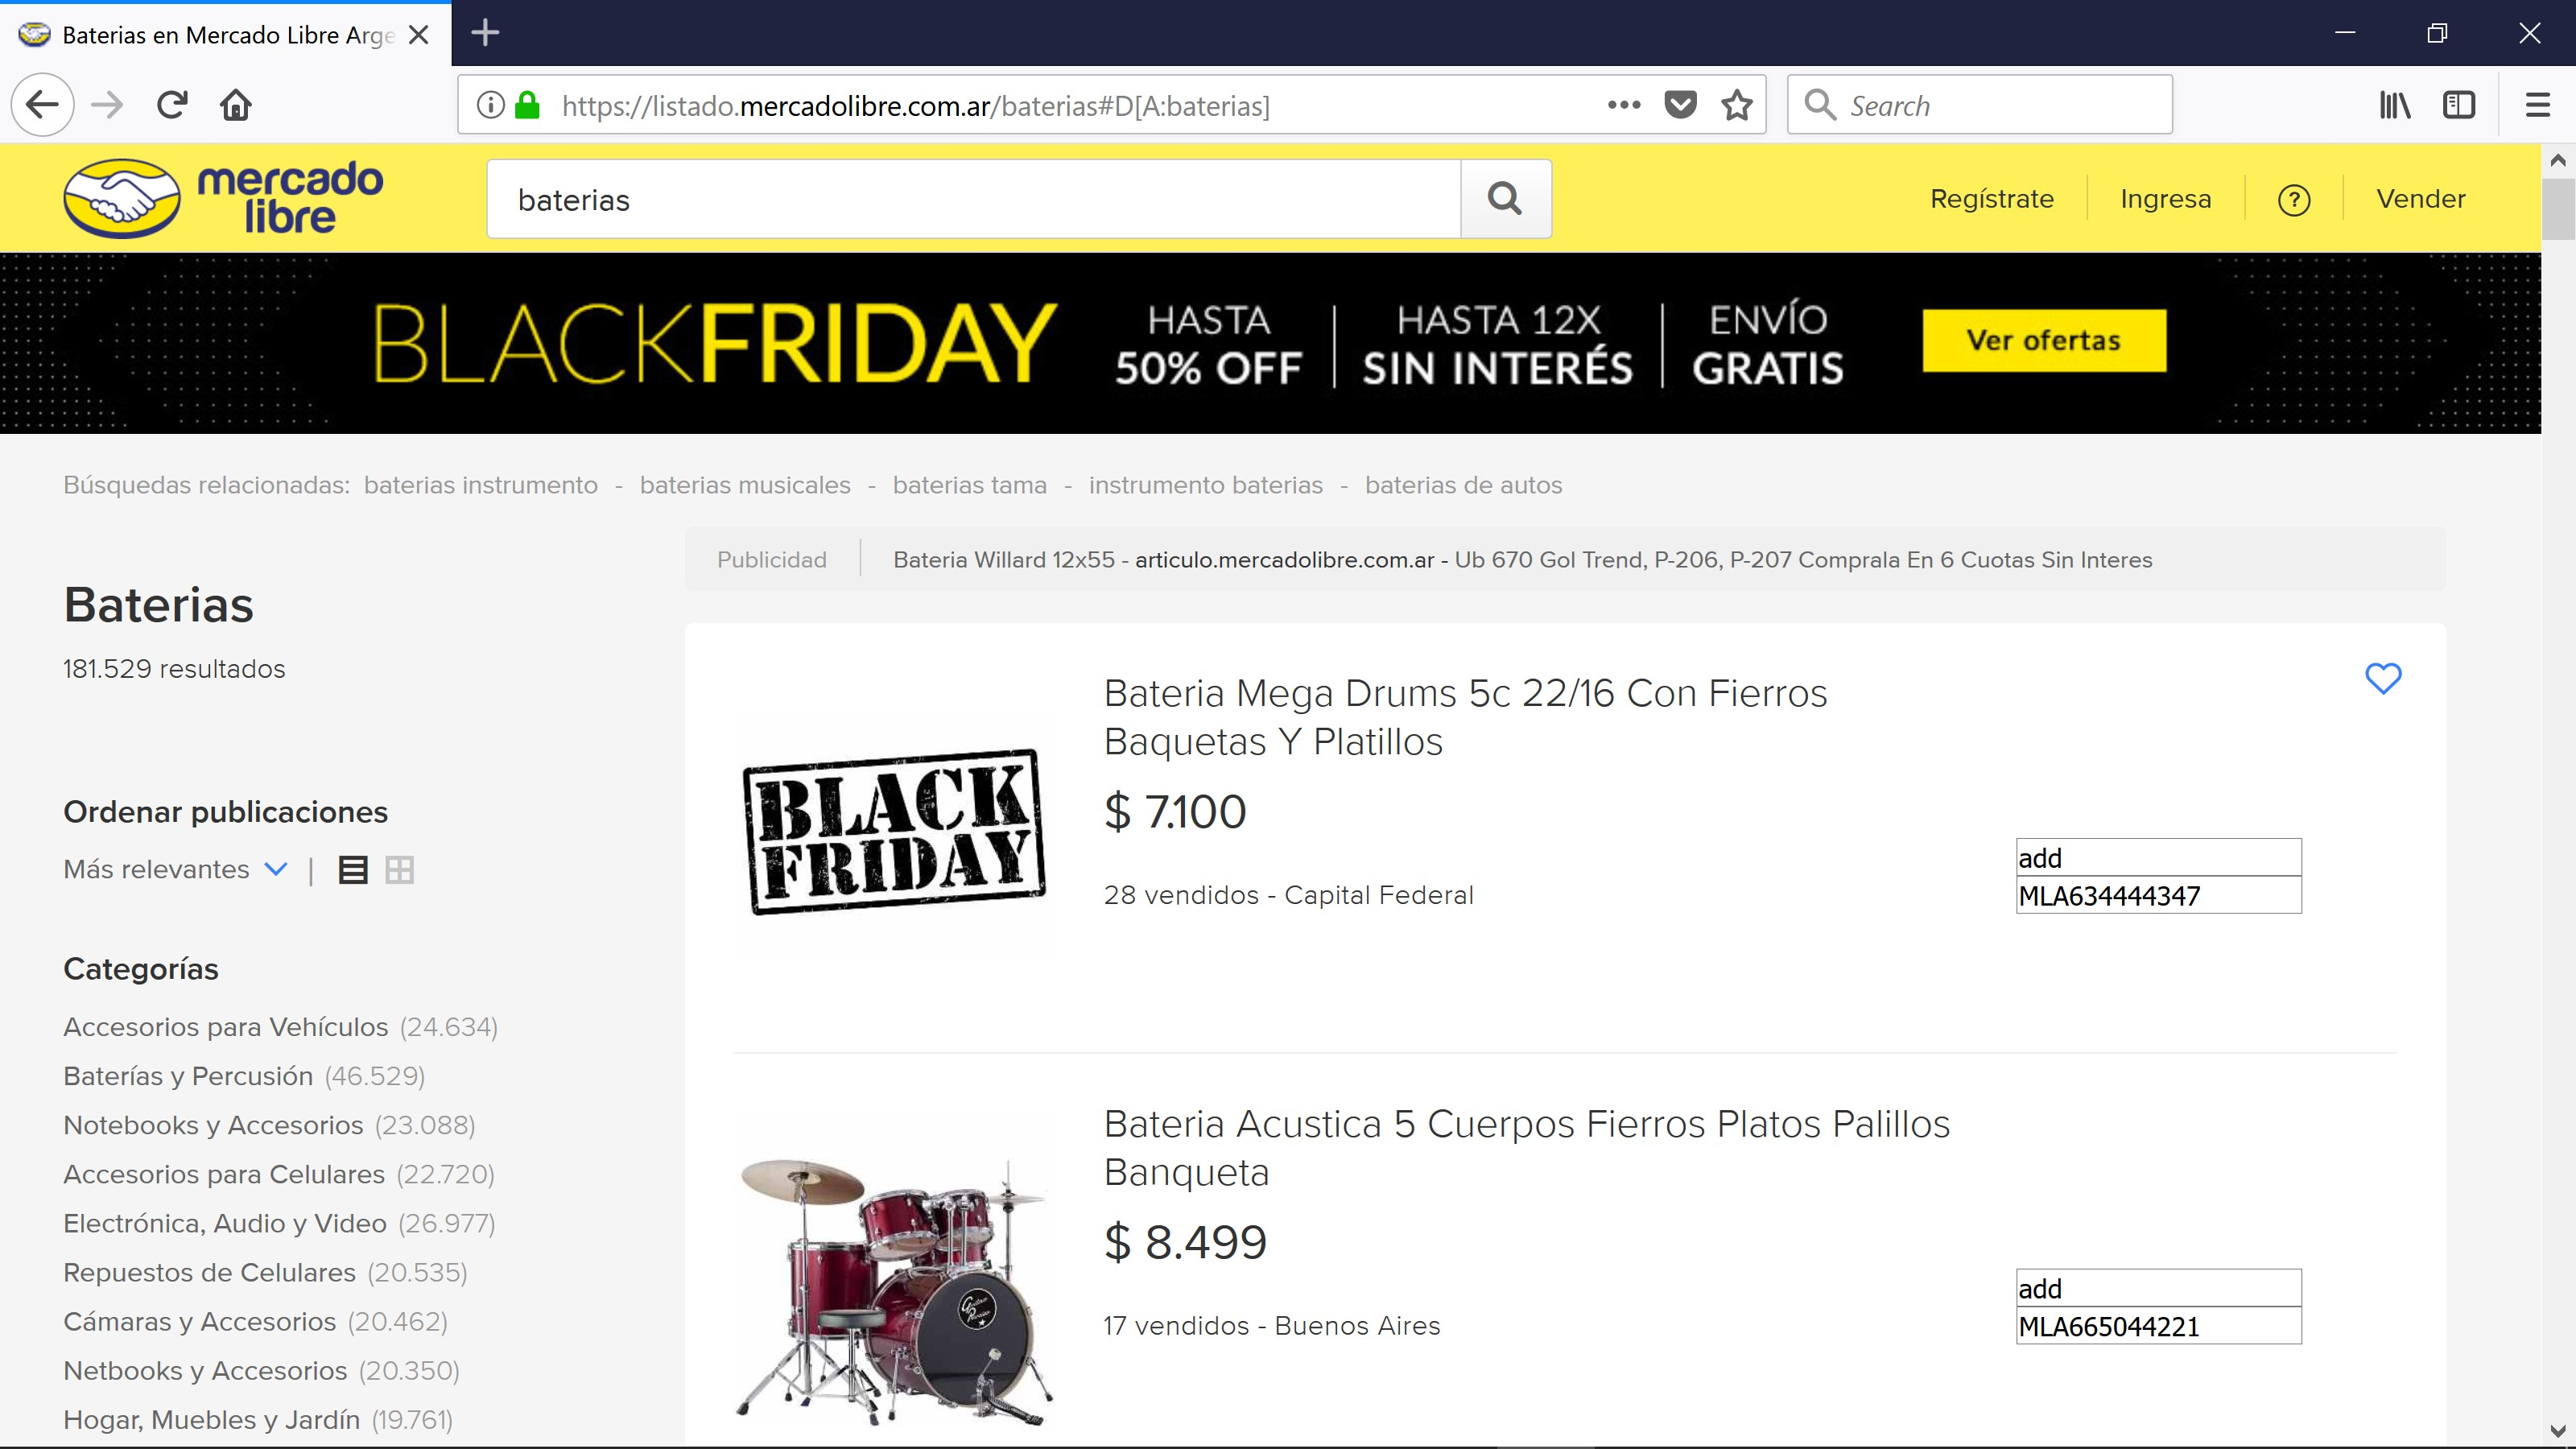
\includegraphics[scale=0.19]{images/ml_1.jpg}}
\caption{}
\end{figure}
Después\newline
\begin{figure}[H]
\centerline{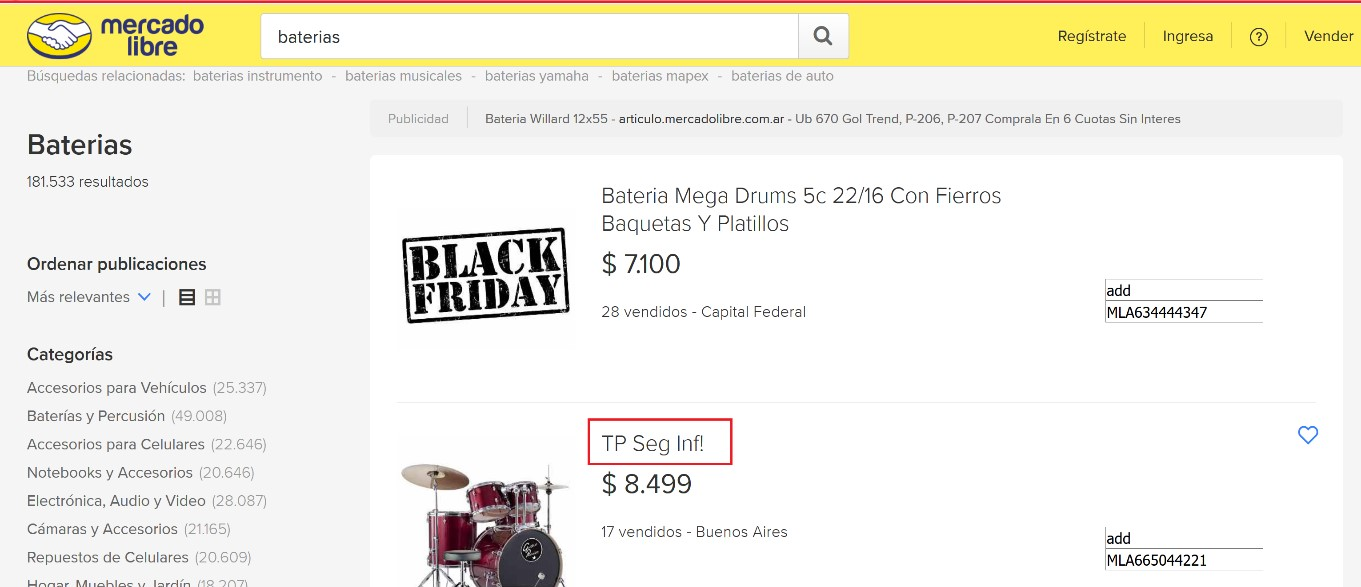
\includegraphics[scale=1]{images/ml_2.jpg}}
\caption{}
\end{figure}

Sobre el mismo sitio también realizamos el ataque de SSLStrip utilizando la misma herramienta.
%También sobre el sitio de MercadoLibre, realizamos un ataque
%denominado \textit{ssltrip} utilizando la herramienta. Dentro de la solapa opciones, está la posibilidad de cambiar automáticamente todo el tráfico https por http.

\begin{figure}[H]
\centerline{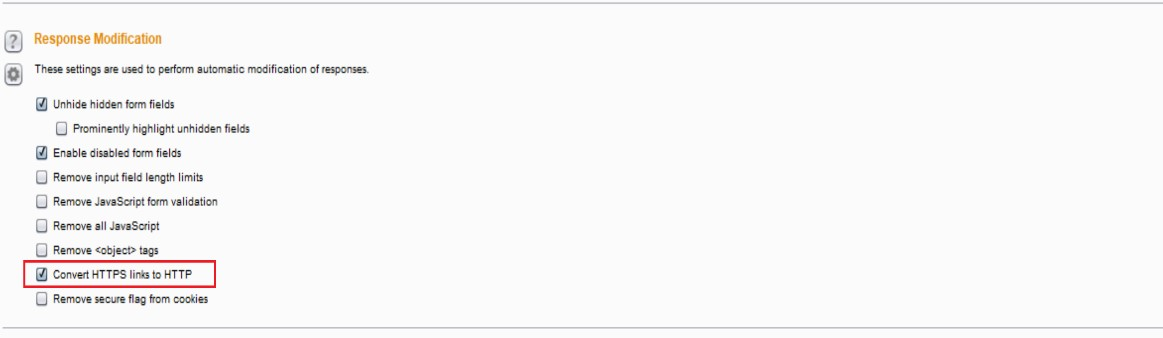
\includegraphics[scale=1]{images/ssltrip.jpg}}
\caption{}
\end{figure}
\begin{figure}[H]
\centerline{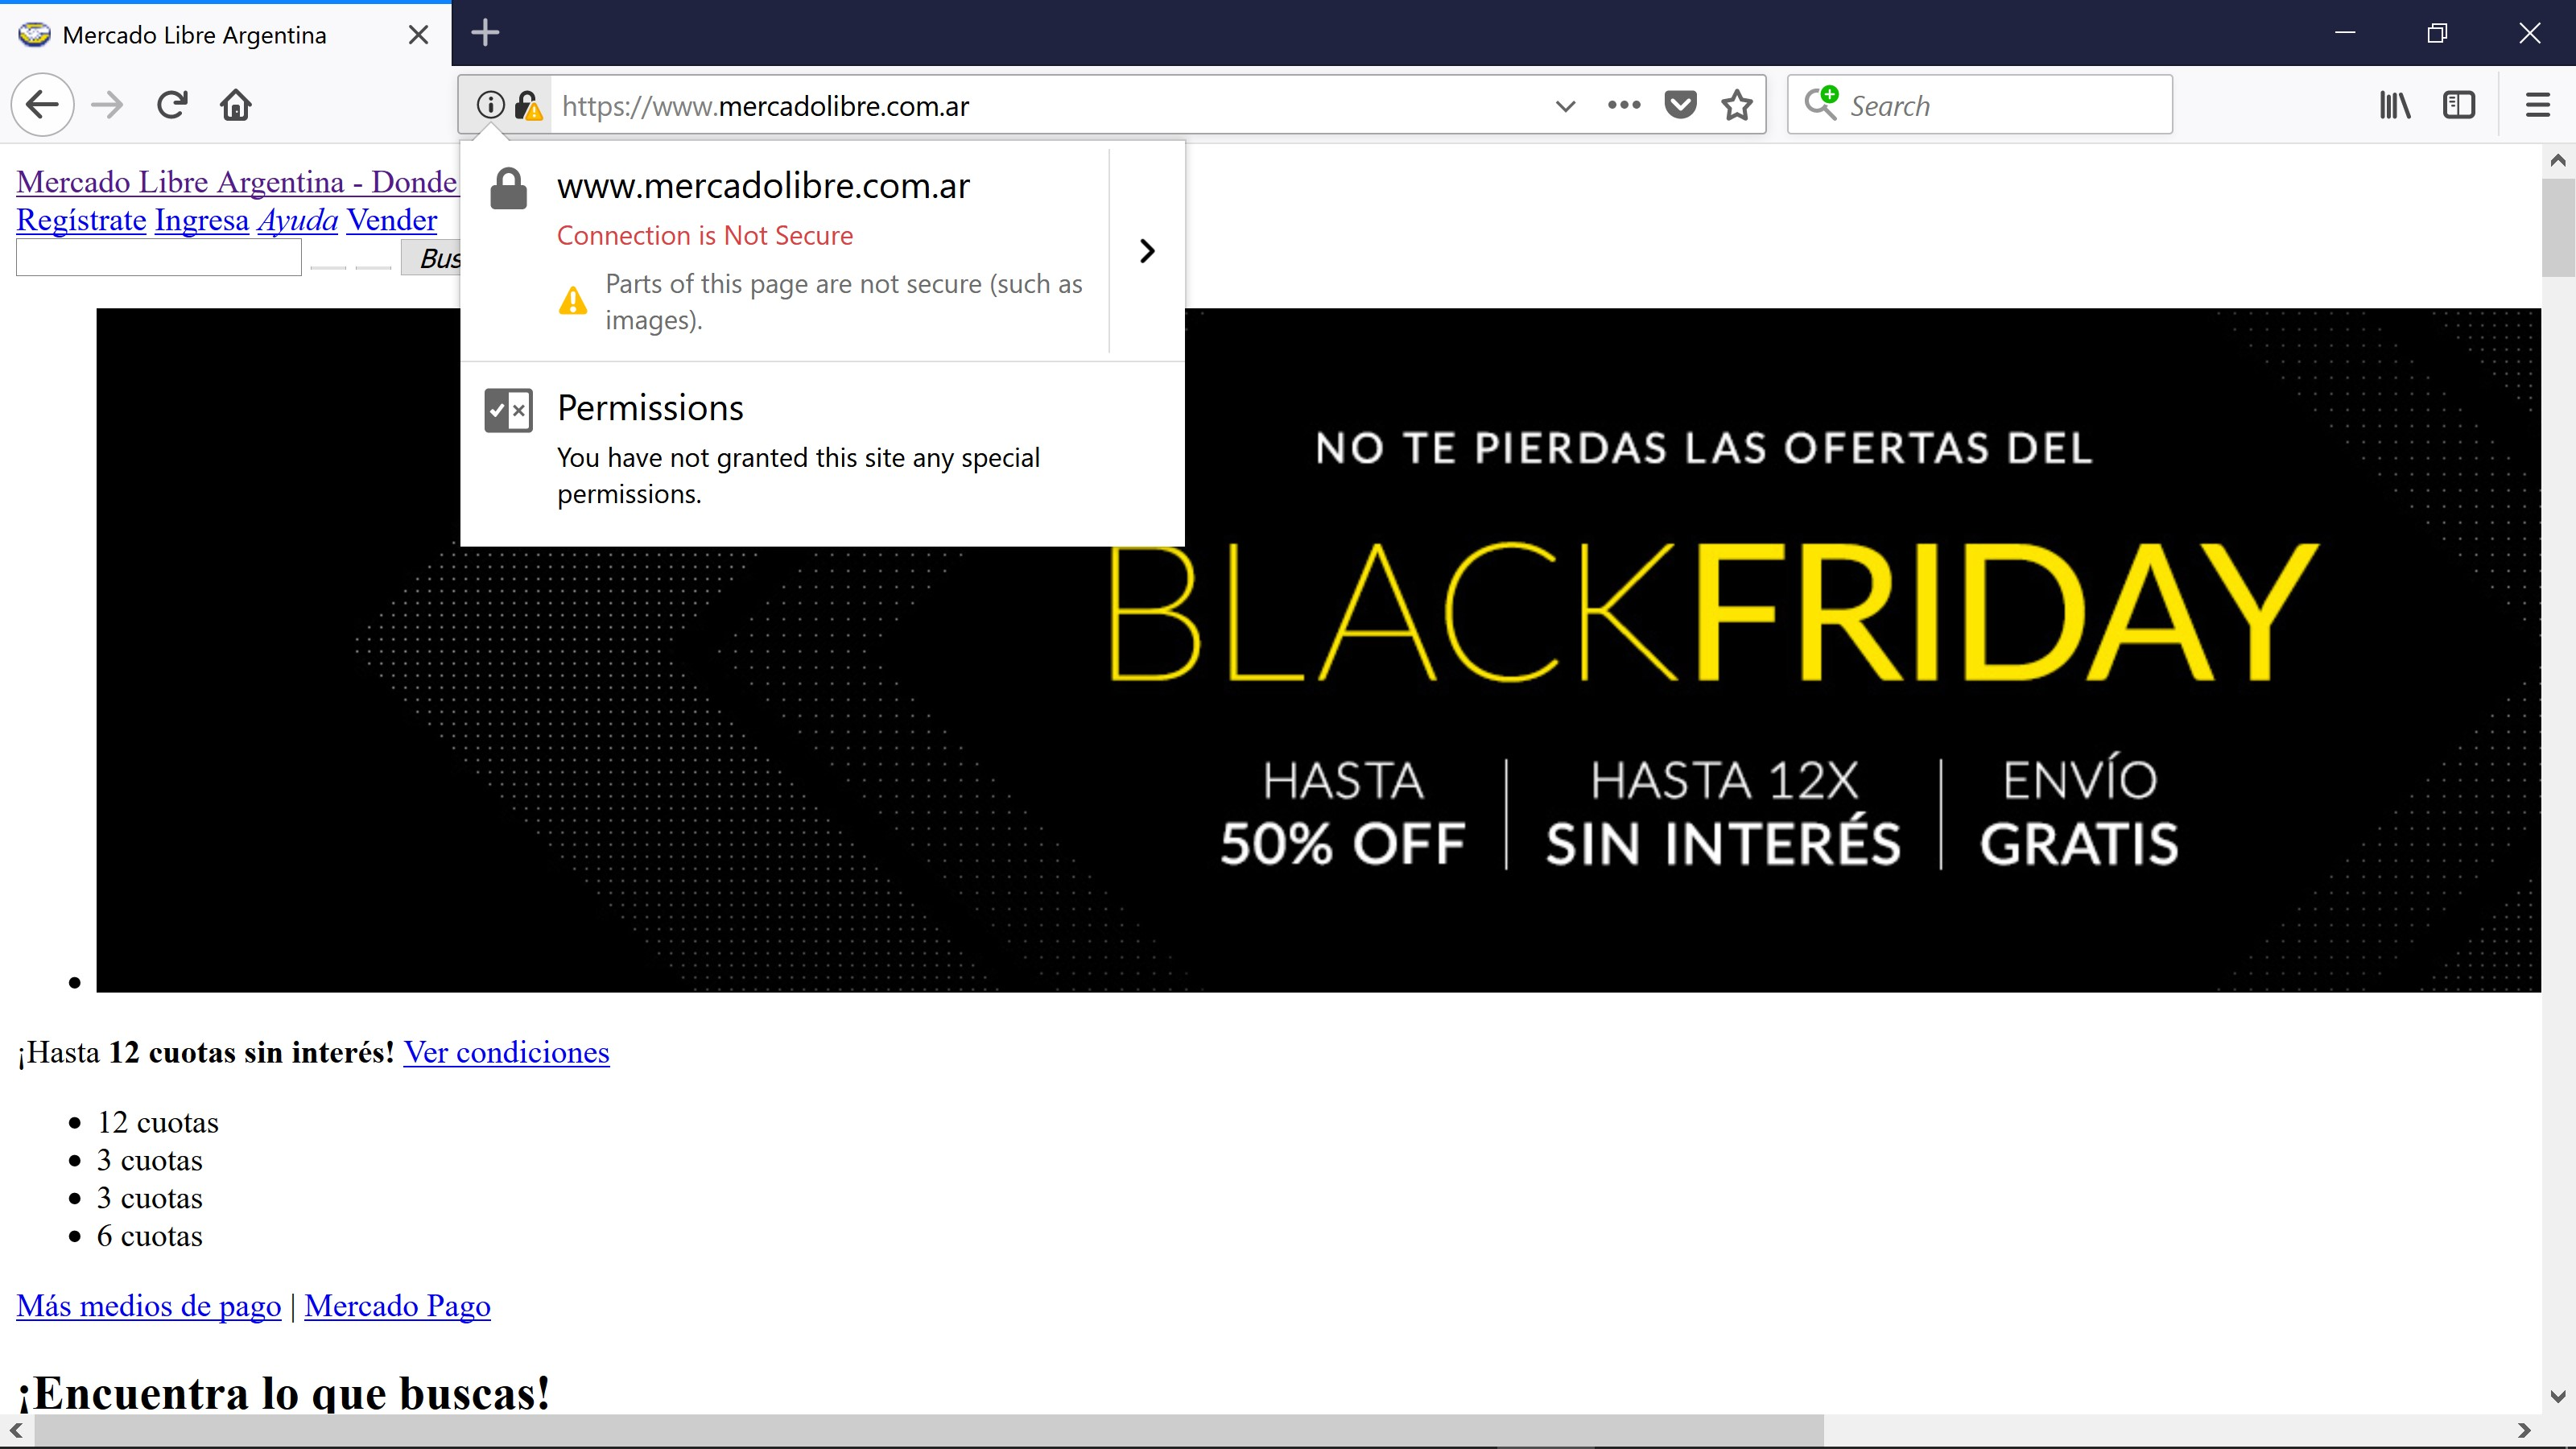
\includegraphics[scale=.2]{images/ml_ssltrip.jpg}}
\caption{}
\end{figure}

Como observamos, la página se cargó incompleta, esto es debido a que los links https que fueron cambiados por el ataque a http no existen (hojas de estilo, urls, imágenes, etc). En estos casos, un atacante podría generar dicho sitio y realizar alguna especie de ataque sobre el dispositivo.

\subsection{Plugin Ettercap}

Como ya hemos mencionado anteriormente existen muchísimas herramientas para hacer análisis sobre redes (algunas incluyen ataques también) y sobre varios SO distintos (Bettercap, Ettercap, Burp, Wireshark, etc), una de las características que poseen varias es la posibilidad de incorporar extensiones (generalmente denominadas plugins) abiertas a desarrollar por todo público. Esto consiste en realizar código propio en el lenguaje necesario, cumplir con cierta interfaz que la herramienta brinda y cargarlo dentro del sistema.
%Si todo funciona correctamente, dentro de la interfaz que debemos cumplir existe un método donde la herramienta llama con un mensaje y podemos cambiar, modificar, eliminar el paquete provisto.
En nuestro caso para experimentar sobre esta funcionalidad desarrollamos un \textit{plugin} en \textit{Ubuntu} para \textit{Ettercap} que descarta paquetes con una probabilidad de 0.5.
Para esto lo que hacemos es compilar un archivo en \textit{C} (dado que es el lenguaje soportado por la herramienta) y lo importamos desde la interfaz gráfica de la misma herramienta.
Para esto iniciamos la interfaz gráfica por medio del comando:\\
\textbf{sudo ettercap -G} \\
Luego proseguimos a escanear todas las IPs conectadas a la red.

\begin{figure}[H]
\centerline{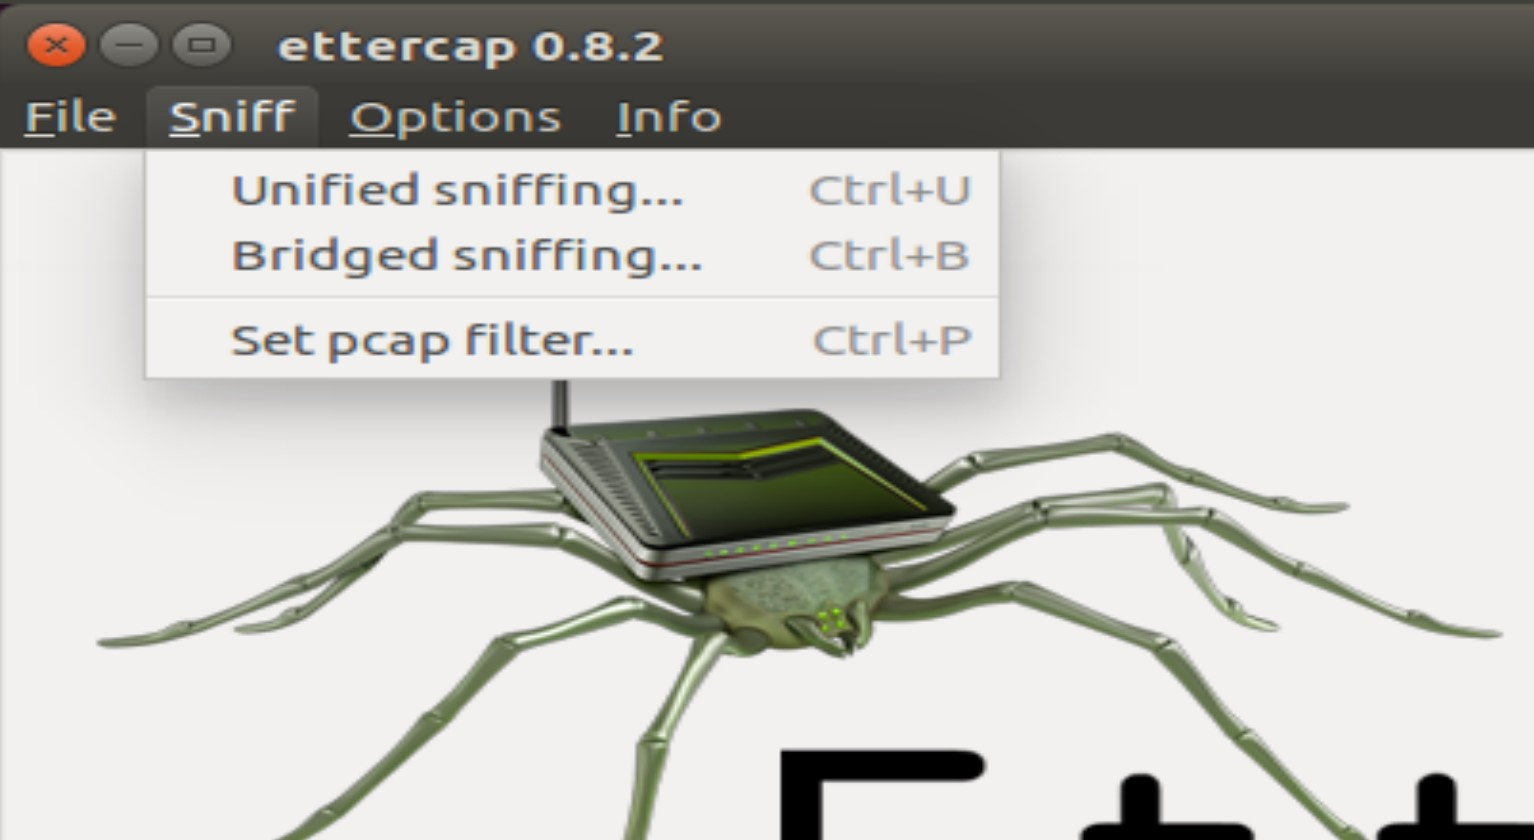
\includegraphics[scale=1]{images/ettercap_1.jpg}}
\caption{}
\end{figure}

Seleccionando la opción \textit{Unified sniffing} y seleccionando la interfaz en la que se quiere realizar la búsqueda. Una vez escaneada la red aparecerá la pestaña de \textit{Plugins} donde podremos seleccionar la opción \textit{Load} para cargar el \textit{plugin} elegido. De esta forma, nuestro \textit{plugin} aparece en el listado. 
\begin{figure}[H]
\centerline{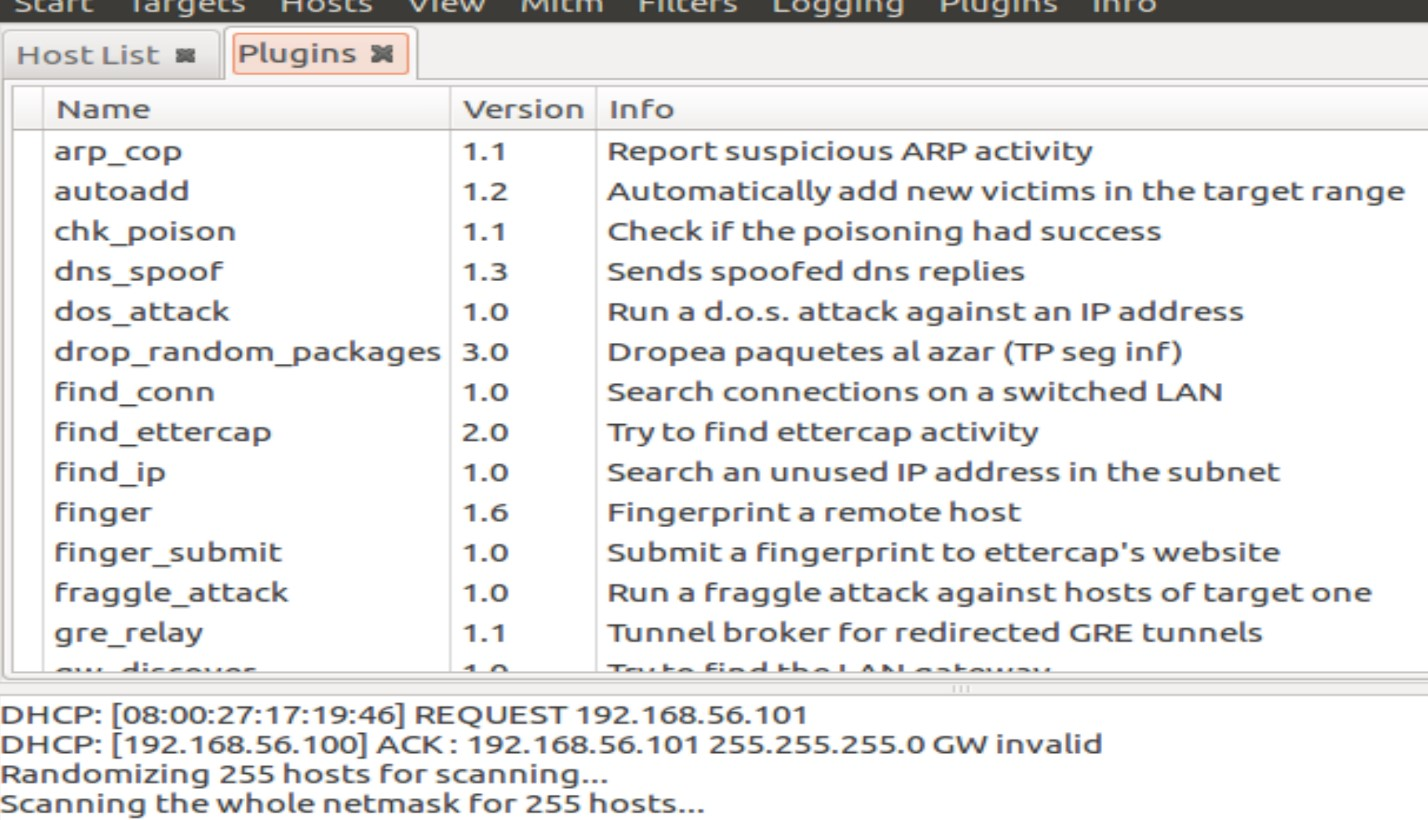
\includegraphics[scale=1]{images/ettercap_plugins_list.jpg}}
\caption{}
\end{figure}

Hacemos doble click sobre el mismo para iniciarlo.

\begin{figure}[H]
\centerline{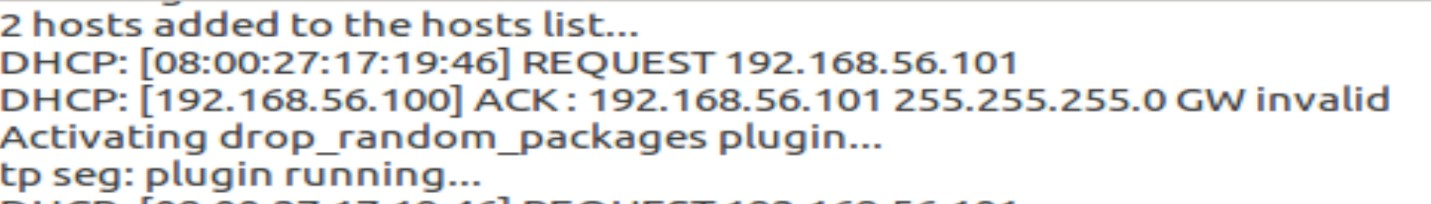
\includegraphics[scale=1]{images/ettercap_plugins_started.jpg}}
\caption{}
\end{figure}

De esta forma, cualquier paquete que pase por la red podrá ser eliminado con cierta probabilidad.

\subsubsection{Código}
\lstinputlisting[language=C]{Codigo/dummy.c}

\pagebreak
\section{Sistemas de Detección de Intrusos}

Los \textit{Sistemas de Detección de Intrusos} (IDS) son sistemas diseñados para vigilar ciertos medios o recursos con el objetivo de identificar y advertir sobre posibles movimientos de algún intento de intrusión. Estos sistemas no siempre suelen ser infalibles ni completamente confiables, debido a que estos dependen de las reglas o heurististicas preestablecidas. A su vez en muchos casos suelen presentar imprecisiones con respecto a la categorización de algunos eventos, de lo cual se desencadenan falsos positivos y falsos negativos. Por esta razón el uso de estos sistemas debe ir acompañado por alguna entidad que tutele y analice toda la información reportada, en especial porque los IDS no incorporan sistemas de prevención o recuperación, por lo cual es importante poder detectar y persistir en reportes a cualquier evento sospechoso lo antes posible. 
Con el objetivo de detectar algunos ataques propuestos anteriormente hemos implementado algunos IDS que trabajan sobre capa de enlace para detectar posibles ataques de KRACK, \textit{ARP Spoofing}, \textit{Deauthentication Attack}, y \textit{Evil Twin}.
\newline

La detección de \textit{Deauthentication Attack} consiste en analizar si un paquete tiene la capa Dot11Deauth de scapy.
Puede haber razones benignas para el uso de este paquete, el detector lo único que hace es registrar estos paquetes en un log.
El usuario luego puede dedicarse a analizar el log y a partir de los datos obtenidos, determinar si hubo un ataque.


La detección de \textit{ARP Spoofing} consiste en registrar si un nodo de la red realiza muchos envíos de paquetes ARP is-at. Si registra más de 10 paquetes de este tipo considera que se está realizando un ataque. Una mejora posible es que cada cierto intervalo de tiempo, limpie los registros, para evitar falsos positivos por el uso normal de la red.

La detección de \textit{Krack} se realiza detectando envíos reiterados del 3er paquete del handshake usando el mismo nonce y diferente número de secuencia de una MAC address a otra.

La detección de \textit{Evil Twin} se realiza detectando beacon frames con igual ssid y diferente bssid.

\subsection{Código}

\subsubsection{ids.py}
\lstinputlisting[language=Python]{Codigo/ids.py}

\subsubsection{ids.py}
\lstinputlisting[language=Python]{Codigo/AttackDetect.py}

\subsubsection{Deauth.py}
\lstinputlisting[language=Python]{Codigo/Deauth.py}

\subsubsection{Arp.py}
\lstinputlisting[language=Python]{Codigo/Arp.py}
\newpage
\subsubsection{Krack.py}
\lstinputlisting[language=Python]{Codigo/Krack.py}

\subsubsection{EvilTwin.py}
\lstinputlisting[language=Python]{Codigo/EvilTwin.py}

\section{Conclusiones}

En base a la investigación y experimentación realizada sobre el funcionamiento de los protocolos y algunas técnicas de ataques, pudimos comprobar que muchos sistemas hoy en día utilizados en dispositivos cotidianos, parecerían no ser examinados previamente por los desarrolladores a la hora de alcanzar cierto nivel de seguridad aceptable, o en muchos casos parecería que directamente la seguridad no fue un tema ni siquiera contemplado. Incluso algunos de aquellos sistemas que, si demostraron tener cierto nivel de seguridad, eran vulnerables a otras técnicas de ataque que no son relativamente nuevas, y para las cuales existe información abierta sobre cómo protegerse. De esto conjeturamos que en muchos casos existe por parte de los desarrolladores o empresas de \textit{software} cierto grado de negligencia a la hora de garantizar la seguridad de datos, de manera que no toman en cuenta la responsabilidad y ni el impacto que esto tiene para con los usuarios de sus servicios. 

\end{document}
